\documentclass[12pt,dvipdfmx]{book}
\usepackage[margin=1in]{geometry}
\usepackage{amsmath,amssymb,amsfonts,mathtools,amsthm}
\usepackage[dvipdfmx]{graphicx}
\usepackage{tcolorbox}
%\usepackage{todonotes}
% 出力PDFバージョンを1.7にする
\usepackage{bxpdfver}
\setpdfversion{1.7}
%\usepackage{slashbox}
%\usepackage{wrapfig}
%\usepackage{url,xspace,ascmac}
%\usepackage[]{xcolor}
%\usepackage{tcolorbox,todonotes}
\tcbuselibrary{breakable, skins, theorems}
%\usepackage{svg}
%\usepackage{etoolbox}
%\usepackage[subrefformat=parens]{subcaption}
%\usepackage{algorithm}
%\usepackage{algorithmic}
\usepackage[normalem]{ulem}
\usepackage{comment,tikz}
%\usepackage{todonotes}
%\usepackage{thmtools,thm-restate}
%\usepackage{enumitem}
%\usepackage{ifthen}
%\usepackage{float}
\addtolength{\textheight}{\topskip}

\usetikzlibrary{positioning,calc}

\tikzset{every picture/.style={font issue=\footnotesize},
            font issue/.style={execute at begin picture={#1\selectfont}}
        }

\usepackage[unicode,colorlinks=true,citecolor=blue,linkcolor=blue,pdfusetitle]{hyperref}
\usepackage[style=alphabetic,natbib=true,natbib=true,maxnames=99,maxalphanames=99,isbn=false,url=false,backref=true,backend=biber,giveninits=true]{biblatex}

%\usepackage[style=alphabetic,natbib=true,maxnames=99,maxalphanames=99]{biblatex}
\addbibresource{ref.bib}

\usepackage{cleveref}

\newcommand{\kara}{} %無を出力するコマンド

%def
\newtcolorbox[auto counter, number within=section, crefname = {定義}{定義}]{definition}[3][]
{enhanced, breakable = true, fonttitle = \bfseries,
title = 定義~\thetcbcounter~\if #2\kara \else(#2) \fi,
#1,
label = def:#3}

%thm
\newtcolorbox[auto counter, use counter from=definition, crefname = {定理}{定理}]{theorem}[3][]
{enhanced, colback = orange!10!white, colframe = red!50!black, breakable = true, fonttitle = \bfseries,
title = 定理~\thetcbcounter~\if #2\kara \else(#2) \fi,
#1,
label = thm:#3}

%prop
\newtcolorbox[auto counter, use counter from=definition, crefname = {命題}{命題}]{proposition}[3][]
{enhanced,  colback = orange!10!white, colframe = red!50!black, breakable = true, fonttitle = \bfseries,
title = 命題~\thetcbcounter~\if #2\kara \else(#2) \fi,
#1,
label = prop:#3}

%lemma
\newtcolorbox[auto counter, use counter from=definition, crefname = {補題}{補題}]{lemma}[3][]
{enhanced,  colback = green!10!white, colframe = green!50!black, breakable = true, fonttitle = \bfseries,
title = 補題~\thetcbcounter~\if #2\kara \else(#2) \fi,
#1,
label = lem:#3}

%cor
\newtcolorbox[auto counter, use counter from=definition, crefname = {系}{系}]{corollary}[3][]
{enhanced, breakable = true, fonttitle = \bfseries,
title = 系~\thetcbcounter~\if #2\kara \else(#2) \fi,
#1,
label = cor:#3}

%remark
\newtcolorbox[auto counter, use counter from=definition, crefname = {注釈}{注釈}]{remark}[3][]
{enhanced, breakable = true, colback = white, fonttitle = \bfseries,
title = 注釈~\thetcbcounter~\if #2\kara \else(#2) \fi,
#1,
label = rem:#3}

%exercise
\newtcolorbox[auto counter, crefname = {演習問題}{演習問題}]{exercise}[3][]
{enhanced, breakable = true, colback = blue!10!white, colframe = blue!50!black, fonttitle = \bfseries,
title = 演習問題~\thetcbcounter~\if #2\kara \else(#2) \fi,
#1,
label = exer:#3}

%conjecture
\newtcolorbox[auto counter, crefname = {予想}{予想}]{conjecture}[3][]
{enhanced, breakable = true, colback = orange!10!white, colframe = orange!60!black, fonttitle = \bfseries,
title = 予想~\thetcbcounter~\if #2\kara \else(#2) \fi,
#1,
label = conj:#3}

\renewcommand{\proofname}{\textbf{証明}}
\renewcommand{\figurename}{図}
\crefname{equation}{式}{式}
\crefname{section}{セクション}{セクション}
\crefname{figure}{図}{図}

\newcommand{\crefrangeconjunction}{--}
\newcommand{\crefpairconjunction}{, }
\newcommand{\crefmiddleconjunction}{, }
\newcommand{\creflastconjunction}{, }

\newcommand{\defeq}{\mathrel{:=}}
\DeclarePairedDelimiter{\abs}{\lvert}{\rvert} % | | absolute value
\DeclarePairedDelimiter{\norm}{\lVert}{\rVert} % || || norm
\DeclarePairedDelimiter{\rbra}{\lparen}{\rparen} % () round brackets
\DeclarePairedDelimiter{\cbra}{\lbrace}{\rbrace} % {} curly brackets
\DeclarePairedDelimiter{\sbra}{\lbrack}{\rbrack} % [] square brackets
\DeclarePairedDelimiter{\abra}{\langle}{\rangle} % < > angle brackets
\DeclarePairedDelimiter{\floor}{\lfloor}{\rfloor} % floor function
\DeclarePairedDelimiter{\ceil}{\lceil}{\rceil} % ceil function

\DeclareMathOperator*{\Epi}{\mathbf{E}_{\pi}}
\DeclareMathOperator*{\Varpi}{\mathbf{Var}_{\pi}}

\newcommand{\indicator}[1]{\mathbf{1}_{#1}}
\newcommand{\condition}{\;\middle\vert\;}
\newcommand{\tand}{\text{ and }}
\newcommand{\tif}{\text{if }}
\newcommand{\totherwise}{\text{otherwise}}

\renewcommand{\vec}[1]{\overrightarrow{#1}}
\newcommand{\e}{\mathrm{e}}
\DeclareMathOperator*{\E}{\mathbb{E}}
\DeclareMathOperator*{\Var}{\mathbb{Var}}
\newcommand{\dtv}{d_{\mathrm{TV}}}
\newcommand{\vG}{\vec{G}}
\newcommand{\tmix}{t_{\mathrm{mix}}}
\newcommand{\LSRW}{\mathrm{LSRW}}
\newcommand{\SRW}{\mathrm{SRW}}
\newcommand{\WSRW}{\mathrm{WSRW}}
\newcommand{\LWSRW}{\mathrm{LWSRW}}
\newcommand{\F}{\mathcal{F}}
\newcommand{\piprod}[1]{\abra*{#1}_{\pi}}
\newcommand{\iprod}[2][X(i)]{\abra*{#2}_{#1}}
\newcommand{\pinorm}[1]{\norm*{#1}_{\pi}}
\newcommand{\piorth}{\bot_{\pi}}
\newcommand{\pispace}{\ell^2_\pi(V)}
\newcommand{\ispace}[1][X(i)]{\ell^2\rbra*{#1}}
\newcommand{\inorm}[2][X(i)]{\norm*{#2}_{#1}}

\newcommand{\pimin}{\pi_{\min}}
\newcommand{\diam}{\mathrm{diam}}
\newcommand{\Fq}{\mathbb{F}_q}
\newcommand{\calG}{\mathcal{G}}
\newcommand{\dist}{\mathrm{dist}}
\newcommand{\Nat}{\mathbb{N}}
\newcommand{\Real}{\mathbb{R}}
\newcommand{\Int}{\mathbb{Z}}
\newcommand{\Comp}{\mathbb{C}}
\newcommand{\binset}{\{0,1\}}
\newcommand{\supp}{\mathsf{supp}\xspace}

\newcommand{\allone}{\mathbf{1}}
\newcommand{\Code}{\mathcal{C}}
\newcommand{\Cay}{\mathrm{Cay}}
\newcommand{\B}{\mathcal{B}}

\newcommand{\Pup}{P^{\uparrow}}
\newcommand{\Pdown}{P^{\downarrow}}
\newcommand{\PUD}{P^{\triangle}}
\newcommand{\PDU}{P^{\bigtriangledown}}
\newcommand{\nonlazyPUD}{P^{\land}}
%\newcommand{\nonlazyPDU}{P^{\vee}}

\title{集中講義:高次元エクスパンダーとその応用}
\author{清水 伸高 (東工大)}
\date{2024年5月}
\begin{document}
\maketitle
\tableofcontents
\renewcommand{\emph}[1]{\textbf{#1}}
\chapter*{序文}
\emph{理論計算機科学 (theoretical computer science)} とは計算機の能力や限界に迫る分野であり, いわゆる応用数学の一つだが, 
    実は純粋数学(特に離散数学)の幅広い分野の概念が登場するいわば「交差点」となるような分野である.
特に近年はグラフ理論におけるエクスパンダー性と呼ばれる性質を単体複体に自然に拡張した
    \emph{高次元エクスパンダー}と呼ばれる概念が近年の理論計算機科学の大きな潮流となっている.

本講義ではまず理論計算機科学においてスタンダードなランダムウォークの定義に基づいてグラフや単体複体上のランダムウォークの理論を構築していき, 高次元エクスパンダーの定義を与え,
Kaufman--Oppenheimの定理やOppenheimのトリクルダウン定理の証明を与える.
そしてマトロイドと呼ばれる離散構造のエクスパンダー性を持つことを証明し, マトロイド上の基交換ウォークの混交性という長年の未解決問題(Mihail--Vazirani予想)の\citet{ALOV24}による証明を与える.

なお, 本講義資料作成にあたって
見村 万佐人先生,
林 興養先生,
来嶋 秀治先生,
平原 秀一先生
に様々な誤植やコメントをいただきました.
この場を借りてお礼申し上げます.

\addcontentsline{toc}{chapter}{Preface}
\chapter{ランダムウォーク概論}
本講義では斉時性をもつ有限状態離散時間マルコフ連鎖をランダムウォークと呼び,
ランダムウォークが収束するために必要な条件を与える.
本チャプターで説明される内容は多くはランダムウォークの非常に有名な教科書\cite[Chapter 4,12]{LP17}にも載っている.

\section{記号}
まず, 本講義の全てのチャプターで共通する記法とその定義を与える.
\begin{itemize}
\item 有限集合$V$上の確率分布$\mu$を$V$次元ベクトルと同一視する.
すなわち, 固定した$u\in V$に対し, 分布$\mu$に従ってランダムに選ばれた元が$u$である確率を$\mu(u)$で表す.
\item 分布$\mu \in [0,1]^V$と部分集合$S\subseteq V$に対し$\mu(S) = \sum_{u\in S}\mu(u)$とする.
\item 有限集合$V$に対して$u\sim V$と書いたとき
\begin{itemize}
\item 集合$V$に何かしらの分布$\mu$が付随しているときは$u$は分布$\mu$に従ってランダムに選ばれた要素であることを意味する. このとき, $u\sim V$の代わりに$u \sim \mu$と書くこともある.
\item そうでない (分布$\mu$が明示的に指定されていない)場合, $u$は$V$上一様ランダムに選ばれたことを意味する.
\end{itemize}
\item 全ての行和が$1$に等しい非負行列を\emph{確率行列 (stochastic matrix)}と呼ぶ.
すなわち, $P \in [0,1]^{U\times V}$が確率行列であるとは, 全ての$u\in U$に対し$\sum_{v \in V} P(u,v) = 1$が成り立つことを意味する.
\item 確率行列$P\in [0,1]^{U\times V}$と$u\in U$に対し, $P(u,\cdot) \in [0,1]^V$を$P$の第$u$行ベクトルから定まる分布とする. 例えば, $v \sim P(u,\cdot)$は分布$P(u,\cdot)$に従ってランダムに選ばれた元を意味する.
\end{itemize}
\section{定義}
%
\begin{definition}{ランダムウォーク}{random walk}
  有限集合$V$と確率行列$P\in[0,1]^{V\times V}$に対し,
  $V$上に値をとる確率変数列$(X_t)_{t\ge 0}$であって, 任意の$t\ge 0$, 頂点列$(v_0,\dots,v_{t-1})\in V^t$,
  および$v\in V$に対して
  \[
    \Pr\sbra*{X_t = v \condition X_0 = v_0,\dots,X_{t-1} = v_{t-1}} = \Pr\sbra*{X_t = v \condition X_{t-1} = u} = P(u,v)
  \]
  を満たすものを$V$上の\emph{ランダムウォーク (random walk)}という.
  特に確率行列$P$をランダムウォーク$(X_t)_{t\ge 0}$の\emph{遷移確率行列 (transition matrix)}と呼ぶ.
\end{definition}
%
初期地点$X_0$もまた確率変数であるためランダムに決まることに注意されたい.
また, 決定的に$X_0=u$からスタートしていても良い.
%
初期頂点$X_0$の分布が決まれば各時刻$t$における$X_t$の分布は一意に定まる.
実際, $t\ge 0$に対し$p_t \in [0,1]^{V}$を$X_t$の分布とする
(すなわち, $p_t(u) = \Pr\sbra*{X_t = u}$).
任意の$t\ge 1$に対し
\begin{align*}
  p_t(v) & = \Pr\sbra*{X_t = v}                                                             \\
         & = \sum_{u\in V}\Pr\sbra*{ X_t = v \tand X_{t-1} = u}                             \\
         & = \sum_{u\in V}\Pr\sbra*{ X_t = v \condition X_{t-1} = u} \Pr\sbra*{X_{t-1} = u} \\
         & = \sum_{u\in V} P(u,v) p_{t-1}(u)
\end{align*}
という漸化式を得る.
これは$p_{t} = p_{t-1} P$とも表せる (ここで$p_t$は行ベクトルとして扱う) ので
\begin{align}
  p_t = p_0 P^t \label{eq:p_t}
\end{align}
を得る.

厳密には初期分布$X_0$と遷移確率行列$P$を定めないとランダムウォークは一意に定まらないが,
しばし遷移確率行列$P$だけを指定して「$P$に従うランダムウォーク」という言い回しをする.
このとき, 暗に初期分布$X_0$は任意の分布を考えており, 例えば「$P$に従うランダムウォークは性質$\mathcal{P}$を満たす」と言ったときは「遷移確率行列が$P$で与えられた任意のランダムウォークは性質$\mathcal{P}$を満たす」ということを意味する.

\section{収束性}
ランダムウォーク$(X_t)_{t\ge 0}$を考え, 時刻$t$における$X_t$の周辺分布を$p_t$とする.
すなわち, $p_t \in [0,1]^V$は$p_t(v) = \Pr\sbra{X_t = v}$で定義されるベクトルである.
本講義では総じて時刻$t$を大きくしていくときの$p_t$の収束性とそのスピードについて議論していく.

まずは収束性について議論するために分布間の距離として全変動距離を導入する.
\begin{definition}{全変動距離}{total variation distance}
  有限集合$V$上の二つの分布$\mu,\nu \in[0,1]^V$に対し, \emph{全変動距離 (total variation distance)}を
  \[
    \dtv (\mu ,\nu ) \defeq \frac{1}{2} \sum_{u\in V}\abs{\mu(u) - \nu(u)} = \frac{1}{2} \norm{\mu - \nu}_1
  \]
  で定める.
\end{definition}
全変動距離は単に$\ell^1$ノルムを$2$で割った値だが, 次の性質を持つがゆえに統計学, 情報理論, 機械学習, 計算機科学を含む様々な分野で非常に重要な役割を果たしている.
\begin{proposition}{}{dtv}
  有限集合$V$を考え, 分布$\pi\in[0,1]^V$と部分集合$U\subseteq V$に対し$\pi(U)\defeq\sum_{u\in U}\pi(u)$とする.
  任意の二つの分布$\mu,\nu\in[0,1]^V$と任意の部分集合$U\subseteq V$に対して
  \[
    \abs*{ \mu(U) - \nu(U) } \le \dtv(\mu,\nu).
  \]
\end{proposition}
すなわち,
全変動距離が小さいということは任意の事象の発生確率の差が小さいことを意味する.
なお, この不等式はタイトである.
実際, $U=\cbra*{ u\in V \colon \mu(u) > \nu(u) }$とすれば等号が成り立つ.

次に, ランダムウォークが収束するための条件を与える.
\begin{definition}{既約性、非周期性}{irreducibility and aperiodicity}
  遷移確率行列$P \in [0,1]^{V\times V}$をもつランダムウォークを考える.
  \begin{itemize}
    \item 任意の頂点対$u,v\in V$に対しある$t \ge 0$が存在して$P^t(u,v)>0$を満たすとき, ランダムウォーク$(X_t)_{t\ge 0}$は\emph{既約 (irreducible)}であるという.
    \item 各頂点$u\in V$に対し, 有向閉路長の集合$L_u = \cbra*{ t \ge 1 \colon P^t(u,u) > 0}$を考え, その最大公約数を頂点$u$の\emph{周期 (period)} と呼ぶ. 全ての頂点の周期が$1$であるとき, ランダムウォーク$(X_t)_{t\ge 0}$は\emph{非周期的 (aperiodic)}であるという.
  \end{itemize}
\end{definition}
%
既約性は任意の頂点対$u,v$に対し$u$からスタートしたランダムウォークが$v$に到達可能であることを意味している.

非周期性は, ランダムウォークが「振動」しないことを意味する性質である.
例えば遷移確率行列が
\[
  P = \begin{bmatrix}
    0 & 1 & 0 \\
    0 & 0 & 1 \\
    1 & 0 & 0
  \end{bmatrix}
\]
で与えられるランダムウォークは全ての有向閉路の長さは$3$の倍数であるためどの頂点の周期も$3$に等しい.
特に, ランダムウォーク$X_t$は周期$3$でループしており, 例えば確率$1$で特定の頂点からスタートしたときに$p_t$は収束しないことがわかる.
非周期性はこのようなケースを排除するという意味を持つ.


\subsection{定常分布}
ランダムウォークの分布$p_t$がある分布$\pi\in[0,1]^V$に収束するならば, 分布の漸化式$p_t = p_{t-1}P$より収束先の分布$\pi$は
\begin{align}
  \pi = \pi P \label{eq:stationary equation}
\end{align}
を満たすはずである.
%
\begin{definition}{定常分布}{stationary distribution}
  遷移確率行列$P$をもつ$V$上のランダムウォークに対し, \cref{eq:stationary equation}を満たす分布$\pi$を\emph{定常分布 (stationary distribution)}と呼ぶ.
\end{definition}
%
任意のランダムウォークは必ず定常分布をもつ.
(有限集合上の分布を考えているので)分布全体から分布全体への連続関数$x \mapsto xP$に対しブラウアーの不動点定理を適用すればすぐに示せる.
\begin{theorem}{ブラウアーの不動点定理}{Brouwer fixed point}
  Euclid空間の非空なコンパクト凸部分集合$K$からそれ自身への任意の連続関数は不動点をもつ.
\end{theorem}
また, 詳細は省くがこれは以下の議論からも証明できる:
\begin{itemize}
  \item 定常分布$\pi$は転置行列$P^{\top}$の固有値$1$の固有ベクトルに対応する.
  \item $P$と$P^\top$の固有値は全て同じ (転置をとっても行列式は変わらないから)であり, 最大固有値$1$を持つ.
  \item Perron--Frobeniusの定理から$P^\top$の最大固有値$1$に対応する固有ベクトルの成分は非負なので, 正規化すると分布になる.
\end{itemize}
%
%
\begin{theorem}{ランダムウォークの収束性}{random walk convergence}
  遷移確率行列$P$を持つ$V$上の任意のランダムウォークは定常分布$\pi \in [0,1]^V$を持つ.
  さらに,
  \begin{itemize}
    \item ランダムウォークが既約的ならば, 定常分布$\pi$は一意に存在し, 全ての頂点$v\in V$に対し$\pi(v)>0$である.
    \item ランダムウォークが既約的かつ非周期的ならば, 定常分布$\pi$が一意に存在して$\dtv(p_t,\pi)\to 0$ ($t\to\infty$)が成り立つ.
  \end{itemize}
\end{theorem}
\cref{thm:random walk convergence}は一つ目の主張は定常分布の定義を使えば簡単に示せるが二つ目の主張の証明は難しい.
そのためにまず, 以下の三つの補題を証明する.
\begin{lemma}{Shurの補題}{Schur lemma}
  $S\subseteq \Nat$が$\gcd(S)=1$ならば, ある$N\in\Nat$が存在して任意の自然数$M\ge N$は$S$の要素の非負結合で表せる.
\end{lemma}
\begin{proof}
  一般性を失わず$S$は有限集合としてよい.
  実際, $S_n = S \cap \{1,\dots,n\}$とすると$\gcd(S_n)$は$n$を大きくしていくにつれて減少していくが, 減少する回数は有限回なので, 十分大きな$n$に対して$\gcd(S_n)=1$となる.
  このとき, $S$の代わりに$S_n$を考えればよい.

  簡単のため$|S|=3$で$S=\{a,b,c\}$のときに証明する.
  一般の$S$の場合も同様に証明できる.
  $\gcd(a,b,c)=1$より,
  任意の$M\in\Nat$に対し
  ある整数$x,y,z\in \Int$が存在して$ax+by+cz=M$を満たす.
  このような$x,y,z$は一意ではなく,
  $i+j+k=0$を満たす任意の$i,j,k\in\Int$に対して
  \[
    a(x+ibc) + b(y+jac) + c(z+kab) = M
  \]
  である.
  ここで, $i,j\in\Int$は任意に決めてよいので, $0\le x+ibc < bc, 0\le y+jac < ac$とできる.
  このときもしも$M\ge 2abc$ならば
  \[
    c(z+kab) = M - a(x+ibc) - b(y+jac) > M - 2abc \ge 0
  \]
  なので, $z+kab \ge 0$であり, 確かに$M$は$a,b,c$の非負結合で表せた.
\end{proof}
\begin{lemma}{}{P bekijou}
  任意の既約的かつ非周期的なランダムウォークの遷移確率行列$P$に対し, ある整数$L \ge 1$が存在して, $P^L$の全ての成分は正となる.
\end{lemma}
\begin{proof}
  遷移確率行列$P$に対し有向グラフ$\vG=(V,\vec{E})$を,
  $P(u,v)>0$のときかつその時に限り有向辺$(u,v)$を追加して得られる有向グラフとする.
  $P^L(u,v)$は, $u$から開始したランダムウォークがちょうど$L$回の遷移の後に$v$にいる確率である.
  この値が正であるということは, $\vG$上で
  $u$から$v$への長さちょうど$L$の有向路が存在することを意味する.

  頂点$w\in V$を任意に固定し, $S\subseteq \Nat$を
  $S = \cbra*{i\ge 0\colon P^i(w,w)>0}$
  とする.
  非周期性より$\gcd(S)=1$である.
  この集合$S$に対し\cref{lem:Schur lemma}により存在性が保証される自然数$N\in\Nat$を考える.
  すると, 任意の$M\ge N$に対して$\vG$は$w$を通る長さ$M$の有向閉路をもつ (つまり$P^M(w,w)>0$).
  
  $L=2|V|+N$が主張を満たすことを示す.
  すなわち, 任意の$u,v\in V$に対し, $\vG$は$u$から$v$への長さ$L$の有向路を含むことを示す.
  既約性の仮定より$\vG$は途中で$w$を経由する長さ$\ell \le 2|V|$の$uv$-有向路$p$を持つ.
  この有向路$p$に沿って$u$から$w$に進み, そこから長さ$L - \ell \ge N$の閉路に沿って進み, さらに再び$p$に沿って$w$から$v$に進む有向路を考えると, その長さはちょうど$L$であり, すなわち$P^L(u,v)>0$を意味する.
\end{proof}
\begin{lemma}{}{ellone norm}
  任意の確率行列$P\in[0,1]^{V\times V}$とベクトル$x\in\Real^V$に対し,
  $\norm{xP}_{1} \le \norm{x}_{1}$.
\end{lemma}
\begin{proof}
  任意の$u\in V$に対し
  \begin{align*}
    \norm{xP}_1 &= \sum_{u\in V} \abs*{(xP)(u)} \\
    &= \sum_{u\in V} \abs*{ \sum_{v\in V} x(v) P(v,u) } \\
    &\le \sum_{u,v\in V}\abs{x(v)}\cdot P(v,u) \\
    &= \sum_{v\in V}\abs{x(v)}\cdot \sum_{u\in V}P(v,u) \\
    &= \norm{x}_1.
  \end{align*}
\end{proof}
\begin{proof}[\textbf{\cref{thm:random walk convergence}の証明.}]
  考えるランダムウォークの遷移確率行列を$P$とする.

  一つ目の主張を示す.
  $P$が既約として, 定常分布の一つを$\pi \in [0,1]^V$とし,
  ある頂点$u\in V$に対し$\pi(u)=0$が成り立つとする.
  $\pi$は分布なのである$v\in V$に対し$\pi(v)>0$となる.
  既約性より, この$v$に対してある$\ell\in\Nat$が存在して$P^\ell(u,v)>0$となる.
  $\pi =\pi P^\ell$より,
  \[
    0 = \pi(u) = \sum_{w\in V}\pi(w)P^\ell(w,u) \ge \pi(v)P^\ell(v,u)>0
  \]
  となり矛盾を得る.

  二つ目の主張を示す.
  $P$は非周期的なので, \cref{lem:P bekijou}より, ある$L\ge 1$に対して$Q\defeq P^L$の全ての成分は正である.
  従って, ある$0<\delta<1$, 全成分が$1/|V|$の確率行列$J$, 適当な確率行列$R$を用いて
  \[
    Q = \delta J + (1-\delta)R
  \]
  と表せる.
  まず定常分布の一意性を示す.
  二つの相異なる定常分布$\pi,\pi'$が存在すると仮定すると
  \begin{align*}
    \norm{\pi - \pi'}_1 = \norm{\pi Q -  \pi' Q}_1 = (1-\delta)\norm{(\pi - \pi')R}_1 \le  (1-\delta)\norm{\pi - \pi'}_1
  \end{align*}
  となるが, これは$\norm{\pi - \pi'}_1>0$に矛盾する (最後の不等号で\cref{lem:ellone norm}を用いた).
  以上より一意性が示された.

  次に収束性を示す.
  $\allone$に直交する任意のベクトルに対し$xQ^t$を考える.
  まず, $t=1$のときは$xQ = (1-\delta) xR$となり, このベクトルもまた$\allone$に直交している.
  実際, $\abra{xR,\allone} = x^\top R \allone = x^\top \allone = 0$である.
  このことから
  $t=2$のときは$xQ^2 = (1-\delta)xR \cdot (\delta J + (1-\delta) R) =(1-\delta)^2 xR^2$を得る.
  これを繰り返していくと, 一般の$t$に対して$xQ^t = (1-\delta)^txR^t$を得る.
  初期分布$p_0\in[0,1]^V$に対し, $x\defeq p_0 - \pi$は$\allone$に直交するので
  \begin{align*}
    \norm{p_t - \pi}_{1} &= \norm{(p_0-\pi)P^t}_{1} \\
    &\le \norm{xQ^{\floor{t/L}}}_{1} & & \text{$\because$\cref{lem:ellone norm}}\\
    &= (1-\delta)^{\floor{t/L}}\cdot \norm{x R^{\floor{t/L}}}_1 \\
    & \le (1-\delta)^{\floor{t/L}} \norm{x}_{1} & & \text{$\because$\cref{lem:ellone norm}} \\
    & \to 0
  \end{align*}
  を得る.
  よって, 確かにランダムウォークの分布$(p_t)$は定常分布$\pi$に収束する.
\end{proof}

\subsection{混交時間}
\cref{thm:random walk convergence}ではランダムウォークの一意収束性の条件を与えた.
では, その収束の速さはどれくらいだろうか?
この問題は日常的には例えば次のような状況で現れる:
\begin{itemize}
  \item トランプカードで遊ぶとき, 何回シャッフルすればカードが「混ざり合う」か?
  \item 料理で調味料をスープに入れたとき, 何回かき回せば味が「混ざり合う」か?
\end{itemize}

ここでは「混ざり合う」とは定常分布への全変動距離の意味での収束性で定義し,
ランダムウォークの混交時間を次で定義する:
\begin{definition}{混交時間}{mixing time}
  既約なランダムウォーク$(X_t)_{t\ge 0}$を考え, $t\ge 0$に対し
  $p_t \in [0,1]^V$を時刻$t$における$X_t$の分布とする.
  定常分布を$\pi \in [0,1]^V$とする.
  正の実数$\varepsilon > 0$に対し, $\varepsilon$-混交時間$\tmix(\varepsilon)$を
  \[
    \tmix(\varepsilon) \defeq \inf\cbra*{ t \ge 0 \colon \dtv(p_t, \pi) \le \varepsilon}
  \]
  とする.
  また, $(1/2)$-混交時間を単に\emph{混交時間 (mixing time)}と呼ぶ.\footnote{$1/2$という数字に特に本質的な意味はない.}
\end{definition}
\begin{remark}{初期分布}{mixing time initial distribution}
  ランダムウォークの混交時間はその初期分布に依存する.
  例えば初期分布が定常分布$\pi$であった場合, 混交時間は$0$である.
  基本的には任意の初期分布を考え, その中で混交時間の最大値を考える.
  任意の分布はディラック測度の凸結合で表せるため,
  全ての初期分布での最大を考える代わりに,
  各ディラック測度(確率$1$で特定の頂点を選択する測度)に関する最大値だけ考えればよい.
  すなわち, 本講義で初期分布を指定していないランダムウォークに対して混交時間の上界を議論する際は
  \[
    \max_{u\in U} \inf\cbra*{ t\ge 0 \colon \dtv(P^t(u,\cdot),\pi) \le \varepsilon }
  \]
  を上から抑えることを意味する.
\end{remark}

本講義では全体を通じてランダムウォークの混交時間(特にその上界)を評価することに取り組む.
中でも特に強力な固有値に基づく解析について説明し,
これに基づいてグラフや単体複体のエクスパンダー性を定義し, その性質を解説していく.
最後にマトロイドと呼ばれる重要な離散構造上のランダムウォークを解析し,
重要な未解決問題であり近年ようやく解決されたMihail--Vazirani予想の証明を与える.

\section{グラフ上のランダムウォーク}
まずグラフ理論の基礎的な概念の定義を与える.
読者は\cref{def:SRW}まで読み飛ばし, 必要に応じて後から定義を参照してもよい.
%
\begin{definition}{グラフ}{graph}
  有限単純無向グラフを単に\emph{グラフ (graph)}と呼ぶ.
  すなわち, グラフとは有限集合$V$とその二元部分集合$E\subseteq \binom{V}{2}$の組 $G = (V, E)$ である.
  $V$の元を\emph{頂点(vertex)}, $E$の元を\emph{辺(edge)}と呼ぶ.
  \begin{itemize}
    \item 二頂点$u,v\in V$が$\{u,v\}\in E$を満たすとき, $u$は$v$に\emph{隣接 (adjacent)}しているという ($v$もまた$u$に隣接している).
          頂点$u$と辺$e\in E$が$u\in e$を満たすとき, $e$は$u$に\emph{接続 (incident)}しているという.
          頂点$u$に隣接している頂点の集合を$N_G(u)$で表す.
          頂点$u$に接続している辺の本数を$u$の\emph{次数(degree)}といい, $\deg(u)$で表す.
          全ての頂点の次数が$d$に等しいとき, $G$は\emph{$d$-正則 ($d$-regular)}であるという.
    \item 二つのグラフ$G=(V,E),H=(U,F)$に対して$U\subseteq V,F\subseteq E \cap \binom{U}{2}$を満たすとき$G$は$H$を\emph{部分グラフ (subgraph)}として含むといい, $H\subseteq G$で表す.
    特に$F=\binom{U}{2}\cap E$となる部分グラフを誘導部分グラフと呼び, $G[U]$と表す.
    \item 隣接行列$A \in \Real^{V\times V}$を以下で定義する:
          \[
            A(u,v) = \indicator{\{u,v\}\in E} =
            \begin{cases}
              1 & \tif\{u,v\}\in E, \\
              0 & \totherwise.
            \end{cases}
          \]
    \item 頂点列$(v_0,\dots,v_\ell) \in V^{\ell+1}$は
          $\{v_0,v_1\},\dots,\{v_{\ell-1},v_\ell\}\in E$を満たすとき,
          $v_0$から$v_\ell$への\emph{路 (walk)} といい, $\ell$を長さと呼ぶ.
          路$(v_0,\dots,v_\ell)$に対し$v_0$と$v_\ell$をそれぞれ始点, 終点と呼ぶ.
          路$(v_0,\dots,v_\ell)$が$v_0=v_\ell$であって満たすものを\emph{閉路 (cycle)}という.
    \item  二頂点$u,v \in V$に対し,
          $u$から$v$への路が存在しかつそのときに限り$u\sim v$
          とすることで頂点集合$V$上の同値関係$\sim$を定義する.
          このとき, 商集合$V / \sim$の各同値類を$G$の\emph{連結成分 (connected component)}という.
          商集合$V / \sim$が単一の連結成分からなるとき, $G$は\emph{連結 (connected)}であるという.
    \item 二頂点$u,v$の間の\emph{距離 (distance)}を, $uv$間の路のうちの最小長さで定義し, $\dist(u,v)$で表す($uv$路が存在しない場合は$\dist(u,v)=\infty$とする). グラフ$G$の\emph{直径 (diameter)}を$\diam(G)=\max_{u,v\in V}\dist(u,v)$で定める.
    \item グラフ$G=(V,E)$を考える.
          二頂点$u,v \in V$に対し,
          $u$から$v$への路が存在しかつそのときに限り$u\sim v$
          とすることで頂点集合$V$上の同値関係$\sim$を定義する.
          このとき, 商集合$V / \sim$の各同値類を$G$の\emph{連結成分 (connected component)}という.
          商集合$V / \sim$が単一の連結成分からなるとき, $G$は\emph{連結 (connected)}であるという.
    \item   グラフ$G=(V,E)$を考える.
          ある頂点分割$V=L\sqcup R$が存在して$E\cap \binom{L}{2}=\emptyset$かつ$E\cap \binom{R}{2}=\emptyset$が成り立つとき, $G$は\emph{二部 (bipartite)}であるといい,
          頂点部分集合$L,R$を$G$の\emph{部集合 (partite set)}と呼ぶ.
  \end{itemize}
\end{definition}
路とは辺を辿って始点から終点に至るまでの経路を表す.
なお, 同じ頂点や辺を2回以上通ってもよいことに注意せよ.

直感的には, $G$が二部グラフであるというのは, ある頂点分割$V=L\sqcup R$に対して
$G$の全ての辺が$L$と$R$の間を跨いでいることを意味する.
なお, 部集合への分割$V = L\sqcup R$は必ずしも一意であるとは限らない.
よく知られる事実として, グラフ$G$が二部グラフであることの必要十分条件は$G$の全ての閉路の長さが偶数であることである.

隣接行列$A$に対し, $A^\ell$の各成分は長さ$\ell$の路の個数に等しい.
\begin{lemma}{}{adjacency walk count}
  グラフ$G=(V,E)$の隣接行列$A$と$\ell\in\Nat$を考える.
  任意の$u,v\in V$に対し, $A^\ell(u,v)$は頂点$u$から$v$への長さ$\ell$の路の個数に等しい.
\end{lemma}
\begin{proof}
  長さ$\ell\ge 1$に関する帰納法で示す. $\ell=1$のときは明らか.
  $W_\ell(u,v)$を頂点$u$から$v$への長さ$\ell$の路の個数とすると, $A^\ell = W_\ell$を示せばよい.
  帰納法の仮定として$A^{\ell - 1} = W_{\ell - 1}$とする.
  $W_{\ell}$に関する漸化式を考える.
  頂点$u$から$v$への長さ$\ell$の任意の路は,
  ある$w\in V$に対して$uw$間の長さ$\ell-1$の路と辺$wv$を連結させることによって得られる.
  従って漸化式$W_\ell(u,v) = \sum_{w \in V} W_{\ell-1}(u,w) \cdot A(w,v)$が成り立つので, 帰納法の仮定より$W_\ell = W_{\ell-1}A = A^\ell$を得る.
\end{proof}

\subsection{単純ランダムウォーク}
単純ランダムウォークとは, 初期地点$X_0$を選び, 現在いる頂点から一様ランダムな隣接点を選びそこに遷移するという
確率的な操作を繰り返して得られるランダムウォークである.
%
\begin{definition}{単純ランダムウォーク}{SRW}
  グラフ$G=(V,E)$を考える.
  遷移確率行列が
  \[
    P_{\SRW}(u,v) \defeq \begin{cases}
      \frac{1}{\deg(u)} & \text{if }\{u,v\}\in E, \\
      0                 & \text{otherwise}
    \end{cases}
  \]
  で与えられる$V$上のランダムウォークを
  $G$上の\emph{単純ランダムウォーク (simple random walk)}という.
\end{definition}
%

単純ランダムウォークの定常分布はの一つは
\begin{align}
  \pi(u) = \frac{\deg(u)}{2|E|}. \label{eq:SRW stationary distribution}
\end{align}
で与えられる.
一般に単純ランダムウォークは既約性や非周期性を持つとは限らない.
既約的であることの必要十分条件はグラフ$G$が連結であることであり,
非周期的であることの必要十分条件はグラフ$G$の全ての連結成分のなす誘導部分グラフが二部グラフでないことである.
実際, 全ての連結成分が二部グラフでないならばそれぞれに長さ奇数の閉路$C$が存在する.
各頂点$u$について, 辺$\{u,v\}$上で$u\to v \to u$という遷移を考えれば長さ$2$の閉路になっている.
また, 頂点$u$から奇閉路$C$に向い, $C$に沿って遷移した後に再び$u$に戻るという経路を考えればこれは奇数長の閉路である.
すなわち$P^2(u,u)>0$かつある奇数$\ell$に対し$P^{\ell}(u,u)>0$となるため頂点$u$の周期は$1$である.
逆に二部グラフならば全ての閉路が偶数長なので任意の奇数$\ell$と頂点$u\in V$に対し$P^\ell(u,u)=0$である.

\subsection{遅延単純ランダムウォーク.}
単純ランダムウォークは二部グラフ上では分布が収束しないという問題点があったが,
これは以下のようにランダムウォークの遷移に自己ループを許容することによって解決することができる.
%
\begin{definition}{遅延単純ランダムウォーク}{lazy SRW}
  グラフ$G=(V,E)$上の単純ランダムウォークの遷移確率行列を$P_{\SRW}$とする.
  確率行列$P_{\LSRW} \defeq \frac{1}{2}(I+P_{\SRW})$を遷移確率行列とする$V$上のランダムウォークを\emph{遅延単純ランダムウォーク (lazy simple random walk)}という. ここで$I$は単位行列.
\end{definition}
要するに遅延単純ランダムウォークとは各頂点に確率$1/2$の自己ループの遷移を許したランダムウォークである.
遷移確率行列の定義より単純ランダムウォークと同じ定常分布を持つ.
自己ループの遷移を許すことによって各頂点の周期が必ず$1$となるため, 遅延単純ランダムウォークは必ず非周期的である.
従って, 連結グラフ上の遅延単純ランダムウォークは\cref{eq:SRW stationary distribution}で与えられる定常分布に一意収束する.

\subsection{グラフ上での上昇ウォークと下降ウォーク} \label{sec:graph up and down walk}
グラフ$G=(V,E)$上の遅延単純ランダムウォークの1回の遷移は次の2つのステップに分解して考えることができる:
\begin{enumerate}
  \item 現在いる頂点$u\in V$に接続している辺$e \in E$を一様ランダムに選ぶ.
  \item 選んだ辺$e$に含まれる二頂点を一様ランダムに選び, その頂点に遷移する.
\end{enumerate}
ステップ1でどの辺を選んだとしてもステップ2で確率$1/2$で元の頂点$u$に戻る.
一方でステップ2で$u$でない方の頂点を選んだ場合は, $u$にとって一様ランダムな隣接点に遷移したことになる.
従ってこの2ステップに基づく遷移は遅延単純ランダムウォークと同じ遷移確率行列をもつ.
ステップ1を頂点$u$から開始したときに辺$e$が選ばれる確率を$\Pup_0(u,e) \in [0,1]^{V \times E}$とし,
同様にステップ2を辺$e$から開始したときに頂点$w \in \{u,v\}$が選ばれる確率を$\Pdown_1(e,w)$とする.
すなわち
\begin{align*}
   & \Pup_0(u,e) = \begin{cases}
                     \frac{1}{\deg(u)} & \text{if }u \in e, \\
                     0                 & \text{otherwise}.
                   \end{cases} \\
   & \Pdown_1(e,w) = \begin{cases}
                       \frac{1}{2} & \text{if }e \ni w, \\
                       0           & \text{otherwise}.
                     \end{cases}
\end{align*}
このとき, 遅延単純ランダムウォークの遷移確率行列$P_{\LSRW}$は$P_{\LSRW} = \Pup_0 \Pdown_1$と表せる.

逆に, 二つのステップを入れ替え, $P'\defeq \Pdown_1 \Pup_0 \in [0,1]^{E\times E}$を遷移確率行列としてもつ$E$上のランダムウォークも考えることができる.
このランダムウォークの遷移は次の2ステップで与えられる:
\begin{enumerate}
  \item 現在いる辺$e = \{u,v\}$に含まれる頂点を一様ランダムに選び$w \in e$とする.
  \item 選んだ頂点$w$に接続している辺$e'\in E$を一様ランダムに選び, その辺に遷移する.
\end{enumerate}
このランダムウォークの遷移確率行列$P'$の対角成分は全て正なので非周期的である.
さらに元のグラフ$G$が連結ならば既約的である.
従って\cref{thm:random walk convergence}より定常分布が一意に存在し, その分布への収束性が成り立つ.
%
\begin{exercise}{}{prob1}
  グラフ$G$が連結であるとする.
  上記の$P'$を遷移確率行列としてもつ辺集合$E$上のランダムウォークの定常分布を求めよ.
  答えだけでよい.
\end{exercise}
%
\begin{proof}[\textbf{解答}]
  定常分布$\pi_E$は$E$上の一様分布となる.
  一意収束性より, $\pi_E(e)\equiv \frac{1}{|E|} $が定常分布の条件を満たすことを確認すればよい. 実際, 各辺$ e\in E $に対して
  \begin{align*} 
      (\pi_E P')(e) &= \rbra*{ \pi_E \Pdown_1 \Pup_0}(e) \\
      &= \sum_{\substack{e' \in E \\ u \in V}} \pi_E(e')\cdot \Pdown_1(e',u)\cdot \Pup_0(u,e) \\
      &= \frac{1}{|E|}\sum_{\substack{e'\in E \\ u \in V}} \frac{\indicator{u\in e'}\cdot \indicator{u\in e}}{2\deg(u)} \\
      &= \frac{1}{|E|}\sum_{u\in e}\frac{1}{2}\sum_{e'\in E\colon e'\ni u}\frac{1}{\deg(u)} \\
      &= \frac{1}{|E|} \\
      &= \pi_E(e)
  \end{align*}
  より, 確かに一様分布$\pi_E$は定常分布である.  
\end{proof}
\subsection{重み付きグラフ上のランダムウォーク}
単純ランダムウォークでは接続している全ての辺は同じ重みを持っている.
各辺に重みと呼ばれる正の実数を割り当てることによって,
重みの大きい辺がより選ばれやすくなるようなランダムウォークを考えることができる.
%
\begin{definition}{重み付きランダムウォーク}{weighted random walk}
  グラフ$G=(V,E)$に対し, 関数$w\colon E\to \Real_{> 0}$を\emph{辺重み (edge weight)}という.
  頂点$u$から$v$に遷移する確率$P(u,v)$が辺重み$w(\{u,v\})$に比例するような$V$上のランダムウォークを\emph{重み付きランダムウォーク (weighted random walk)}と呼ぶ.
  すなわち, 重み付きランダムウォークとは以下の定常分布$P$を持つランダムウォークである:
  \[
    P(u,v) = \begin{cases}
        \frac{w(\{u,v\})}{\deg_w(u)} & \tif \{u,v\}\in E,\\
        0 & \totherwise.
      \end{cases}
  \]
  ここで, $\deg_w(u)=\sum_{v\colon \{u,v\}\in E} w(\{u,v\})$は頂点$u$の重み付き次数とする.
\end{definition}
辺重み$w$を常に$1$を返す関数とすれば, $G$上の単純ランダムウォークと同一である.
自己遷移は発生しないので単純遅延ランダムウォークは表現できない.
重み付きランダムウォークの概念は後で単体複体上での局所的なランダムウォークの定義(\cref{def:local random walk})で用いる.

\begin{comment}
\section{混交時間解析の実例}
講義とは直接な関係はないが,
最後にランダムウォークの混交性解析の応用例をいくつか簡単に説明する.
より深く知りたい読者はLevinとPeresによるこの分野の標準的な教科書\cite{LP17}を参照されたい.

\subsection{到達時間, 全訪問時間の解析}
\subsection{マルコフ連鎖モンテカルロ法}
\subsection{イジングモデル}
\end{comment}

\section{ランダムウォークの固有値と可逆性}
遷移確率行列$P \in [0,1]^{V \times V}$に従う$V$上の既約的かつ非周期的なランダムウォーク$(X_t)_{t\ge 0}$を考え,
その一意な定常分布を$\pi$とする.
\Cref{thm:random walk convergence}より収束性が保証されるが, その速さを遷移確率行列の固有値に基づいて評価できる.

遷移確率行列$P \in [0,1]^{n \times n}$の固有値
\footnote{本講義では左固有値, すなわち$Px=\lambda x$を満たす$\lambda\in \Comp$を考える.}
$\lambda_1,\dots,\lambda_n$について考える.
全ての成分が$1$であるベクトル$\allone\in \Real^n$を考えると$P\allone = \allone$であるから
$P$は固有値$1$を持つ.
さらに, 以下が成り立つ:
\begin{theorem}{遷移確率行列の固有値}{random walk eigenvalue}
    任意の遷移確率行列$P\in [0,1]^{n\times n}$の固有値を$\lambda_1,\dots,\lambda_n$とすると,
    全ての$i\in\{1,\dots,n\}$に対して$\abs{\lambda_i} \le 1$を満たす.

    さらに, $P$が既約的かつ非周期的なランダムウォークの遷移確率行列とすると,
    固有値$1$の多重度は$1$であり, 他の固有値は全て絶対値が真に$1$より小さい.
\end{theorem}
\begin{proof}
  まず一つ目の主張を示す.
  $P$の任意の固有値$\lambda \in \Comp$を考え, 対応する固有ベクトルを$f \in \Comp^V$とする.
  頂点$u\in V$を, $\abs{f(u)}$が最大となる頂点とすると
  \begin{align*}
    \abs{\lambda} \abs{f(u)} &= \abs*{(Pf)(u)} \\
    &\le \sum_{v\in V} P(u,v) \abs*{f(v)} \\
    &\le \abs{f(u)}\cdot \sum_{v\in V} P(u,v) \\
    &= \abs{f(u)}
  \end{align*}
  より, 両辺を$\abs{f(u)}>0$で割ると$\abs{\lambda}\le 1$を得る.

  二つ目の主張を示す.
  $P$を既約的かつ非周期的なランダムウォークの遷移確率行列とする.
  $J\in\Real^{V\times V}$を全成分が$1/n$の行列とする.
  \cref{lem:P bekijou}より, ある$L\in\Nat,\delta\in (0,1)$および確率行列$R\in[0,1]^{V\times V}$が存在して, $Q\defeq P^L$は
  \[
    Q = \delta J + (1 - \delta) R
  \]
  と表せる (ここで$J$は全成分が$1/|V|$の確率行列).
  $f\in \Comp^V$を$P$の第一以外の任意の固有値$\lambda$に対する固有ベクトルとする.
  すなわち, $f$は何らかの定数$c\in\Comp$に対し$f=c\allone$の形になって\emph{いない}固有ベクトルである.
  二頂点$u,v\in V$を$\abs{f(u) - f(v)}$が最大となるようにとる.
  $f$の取り方の仮定から$\abs{f(u) - f(v)} > 0$である.
  すると, $f$は$Q$の固有値$\lambda^L$に対応する固有ベクトルなので
  \begin{align*}
    \abs{\lambda^L}\abs{f(u) - f(v)} &= \abs*{(Qf)(u) - (Qf)(v)} \\
    &= (1-\delta)\abs*{(Rf)(u) - (Rf)(v)} \\
    &= (1-\delta) \abs*{ \sum_{w\in V}R(u,w)f(w) - \sum_{w\in V} R(v,w)f(w)} \\
    &\le (1-\delta)\max_{w,w'\in V}\abs*{f(w) - f(w')} \\
    &=(1-\delta)\abs{f(u) - f(v)}.
  \end{align*}
  四行目の不等号では$\sum_{w\in V}R(u,w)f(w)$が各$f(w)$の凸結合で表せることを用いた.
  両辺を$\abs{f(u) - f(v)} > 0$で割って整理すれば$\abs{\lambda^L}<1$を得る.
\end{proof}
%

ランダムウォークの固有値の議論の土台となるのが可逆性という概念である.
一般の遷移確率行列は対称とは限らないが, 可逆性を仮定することによって
遷移確率行列を対称行列として扱うことができ,
対称行列に対して展開される固有値分解などの理論を同じように
遷移確率行列に対しても適用することができる.
%
\begin{definition}{可逆性}{reversible}
    遷移確率行列$P$を持つ$V$上のランダムウォークは,
    ある$V$上の分布$\pi \in [0,1]^V$が存在して
    \begin{align}
        \forall u,v\in V,\pi(u) P(u,v) = \pi(v) P(v,u) \label{eq:reversible}
    \end{align}
    を満たすとき\emph{可逆 (reversible)}であるという.
\end{definition}
\cref{eq:reversible}で表される条件を\emph{詳細釣り合い条件 (detailed balanced equation)}という.
分布$\pi\in [0,1]^V$を対角成分に並べた対角行列$\Pi\in[0,1]^{V\times V}$を用いると
$(\ref{eq:reversible}) \iff \Pi P = (\Pi P)^{\top}$
となる.

可逆性とは直感的に言うと, 逆再生しても同じ分布のランダムウォークになるという性質である.
ランダムウォーク$(X_t)_{t\ge 0}$であって初期頂点$X_0$が分布$\pi$に従って選ばれたものを考えよう.
適当な時刻$t=T$で打ち切って得られる頂点列$(X_0,\dots,X_T)$に対し, 順序を逆にした系列
$(X_T,\dots,X_0)$はランダムウォークから得られた系列と見做せるだろうか?
仮にこれがある遷移確率行列$P^*\in[0,1]^{V\times V}$に従うランダムウォークであったとしよう.
簡単のため$T=1$とする ($T\ge 2$に関しても同じ議論が適用できる).
初期頂点$X_0$の分布$\pi$が定常分布だとすると, $X_1$の分布も$\pi$である.
また, ランダムウォークの条件から$\Pr[X_1 = v \tand X_0=u] = \pi(u)P(u,v)$である.
従って条件付き確率の定義より
\begin{align}
    P^*(v,u) = \Pr[X_0 = u | X_1 = v] = \frac{\Pr[X_0 = u \tand X_1 = v]}{\Pr[X_1 = v]} = \frac{\pi(u)P(u,v)}{\pi(v)} \label{eq:reversal chain}
\end{align}
が得られる.
もし元のランダムウォークが可逆ならば, \cref{eq:reversible}から$P^*=P$を得る.
すなわち, ランダムウォークの可逆性とはそのランダムウォークが時間反転に関して対称性を持つことを意味する.
なお, \cref{eq:reversal chain}で得られる遷移確率行列に従って生成されるランダムウォークを\emph{時間反転ランダムウォーク (time-reversal random walk)}と呼ぶ.

なお, 後の節(\cref{sec:Rayleigh quotient})で可逆なランダムウォークに対する\cref{thm:random walk eigenvalue}を証明する.

\paragraph*{例1.単純ランダムウォーク}
連結グラフ$G=(V,E)$上の単純ランダムウォークを考えよう.
\cref{eq:SRW stationary distribution}で与えられる定常分布を$\pi$とすると
任意の二頂点$u,v\in V$に対して
\[
    \pi(u) P(u,v) = \frac{\deg(u)}{2|E|} \cdot \frac{\indicator{\{u,v\}\in E}}{\deg(u)}
    = \frac{\deg(v)}{2|E|} \cdot \frac{\indicator{\{u,v\}\in E}}{\deg(v)}
    = \pi(v) P(v,u)
\]
より, 単純ランダムウォークは可逆である (連結なので全ての頂点に対して$\deg(u)>0$である).
ここで, $\indicator{\dots}$は指示関数である.
同様に, 重み付きランダムウォークもまた可逆である.

\paragraph*{例2.有向グラフ上のランダムウォーク}
可逆で\emph{ない}例として次の遷移確率行列で与えられるランダムウォークを考えてみよう:
\begin{align*}
    P = \begin{pmatrix}
            0 & 1 & 0 \\
            0 & 0 & 1 \\
            1 & 0 & 0
        \end{pmatrix}.
\end{align*}
この例は遷移が決定的なのでランダムウォークとしては面白くないが,
次のようにして可逆でないことが確認できる:
頂点集合を$V=\{0,1,2\}$とし, $i\in V$に対して$(i+1)\bmod 3$を省略して$i+1 \in V$と書くと
\begin{align*}
    \pi(i) = \pi(i) P(i, i+1) = \pi(i+1)P(i+1,i) = 0
\end{align*}
より$\pi=0$となってしまい, 分布であることに矛盾.

\begin{exercise}{}{prob2}
    可逆なランダムウォークの遷移確率行列を$P$とする.
    \cref{eq:reversible}を満たす分布$\pi$は定常分布であることを示せ.
\end{exercise}
\begin{proof}[\textbf{解答}]
  等式$\pi P = \pi$を示せばよい.
  各頂点$u \in V$に対し,
    \begin{align*} 
       (\pi P) (u) &= \sum_{v\in V}\pi(v) P(v,u) \\
       &= \sum_{v\in V} \pi(u)P(u,v) & & \because\text{\cref{eq:reversible}} \\
       &= \pi(u) & & \because \sum_{v\in V}P(u,v)=1
    \end{align*}
    より主張を得る.
\end{proof}

\section{定常分布から定まる内積とノルム}
可逆なランダムウォークは遷移確率行列の固有値を考える上で非常に扱いやすいランダムウォークのクラスとなっている.
ランダムウォークの分布は遷移確率$P$を右から掛けて得られるのに対し,
固有値に基づく議論では左固有値を考えており,
この左右の差異に違和感を覚える読者もいるであろう.
実は可逆なランダムウォークでは遷移確率行列を対称行列のように扱うことができ,
ゆえに左右どちらから作用させようが本質的に同じとなる.
このことを説明するために, $\Real^V$に次の内積を導入する.
\begin{definition}{}{naiseki}
    有限集合$V$上の分布$\pi\in(0,1]^V$に対し,
    $\Real^V$に以下の内積$\piprod{\cdot,\cdot}$を定めた内積空間を$\pispace$で表す:
    \begin{align*}
        \piprod{f,g} \defeq \sum_{u \in V} \pi(u) f(u) g(u)
        = f^\top \Pi g.
    \end{align*}
    ここで$f,g$は列ベクトルとして扱い, $\Pi=\mathrm{diag}(\pi)$はベクトル$\pi$の成分を対角に並べた行列である.
    また, 内積$\piprod{\cdot,\cdot}$が誘導するノルムを$\pinorm{\cdot}$で表す.
    すなわち, $f\in\Real^V$に対して
    \[
        \pinorm{f} \defeq \sqrt{\piprod{f,f}}.
    \]
    %    二つのベクトル$f,g \in \Real^V$が$\piprod{f,g} = 0$であるとき, $f \piorth g$で表す.
\end{definition}
\cref{def:naiseki}で考える分布$\pi$は全ての成分が正であるため,
上記の内積$\piprod{\cdot,\cdot}$はちゃんと実ベクトル空間の内積の公理(対称双線形性, 非退化性, 半正定値性)を満たしており,
確かに$\pispace$は内積空間である.

$\Real^V$上の通常の内積$\abra{\cdot,\cdot}$を考えたとき, 任意の対称行列$M \in \Real^{V\times V}$とベクトル$f,g\in \Real^V$に対して $\abra{f,Ag} = \abra{Af,g}$
が成り立っていたが,
可逆なランダムウォークの遷移確率行列$P$は内積$\piprod{\cdot,\cdot}$に関して同様の性質を持つ.
\begin{lemma}{}{reversible adjoint}
    定常分布$\pi$をもつ既約的かつ可逆なランダムウォークの遷移確率行列$P$は,
    任意の$f,g\in\Real^V$に対して
    \[ \piprod{f,Pg} = \piprod{Pf,g} \]
    を満たす.
\end{lemma}
\begin{proof}
    定常分布$\pi$を対角成分に並べた対角行列$\Pi$を考えると
    \begin{align*}
        \piprod{f,Pg} & = f^\top \Pi P g                                              \\
                      & = f^\top (\Pi P)^\top g &  & \text{$\because$可逆性より$\Pi P$は対称} \\
                      & = (Pf)^\top \Pi g       &  & \text{$\because\Pi^\top = \Pi$}  \\
                      & = \piprod{Pf,g}.
    \end{align*}
\end{proof}
一般に$P$が可逆とは限らない場合,
\cref{eq:reversal chain}で与えられる時間反転ランダムウォークの遷移確率行列$P^*$に対し$\piprod{f,Pg} = \piprod{P^*f,g}$が成り立つ.
この意味で$P^*$は$P$の随伴とみなすことができる.


対称行列に対して展開される固有値分解などの理論は可逆なランダムウォークの遷移確率行列に対しても同様に展開できる.
例えば, 対称行列と同様に可逆なランダムウォークの遷移確率行列は実固有値をもつ.
\begin{lemma}{実固有値性}{reversible real eigenvalue}
    既約的かつ可逆なランダムウォークの遷移確率行列$P$と定常分布$\pi$に対し,
    行列
    \begin{align}
        A \defeq \sqrt{\Pi} P \sqrt{\Pi}^{-1} \label{eq: symmetrized P}
    \end{align}
    を考える.
    $P$と$A$は(多重度も含め)同じ固有値をもち, これらは全て実数である.
\end{lemma}
\begin{proof}
    行列$A$は対称である.
    実際,
    \begin{align*}
        A^\top & = \sqrt{\Pi}^{-1} P^{\top} \sqrt{\Pi}                            &  & \text{$\because$$\sqrt{\Pi},\sqrt{\Pi}^{-1}$は対称} \\
               & = \sqrt{\Pi} \cdot \Pi^{-1} P^{\top} \Pi \cdot \sqrt{\Pi}^{-1}                                                         \\
               & = \sqrt{\Pi} \cdot \Pi^{-1} (\Pi P)^{\top} \cdot \sqrt{\Pi}^{-1}                                                       \\
               & = \sqrt{\Pi} \cdot \Pi^{-1} \Pi P \cdot \sqrt{\Pi}^{-1}          &  & \text{$\because$可逆性より$\Pi P$は対称}                 \\
               & = A.
    \end{align*}
    $A$は対称なので全ての固有値は実数である.

    $A$と$P$は相似なので多重度も含めて同じ固有値をもつ. 実際,
    $A$の固有値$\lambda$に対する固有ベクトルを$x$とし, ベクトル$y\defeq \sqrt{\Pi}^{-1}x$を考える.
    固有ベクトルの式
    \begin{align*}
        A x = (\sqrt{\Pi} P \sqrt{\Pi}^{-1})x =  \lambda x
    \end{align*}
    の両辺に左から$\sqrt{\Pi}^{-1}$を掛けると
    \begin{align*}
        P y = \lambda y
    \end{align*}
    を得る.
    すなわち, $P$と$A$は同じ固有値を持つ.
    特に, $P$の固有値も全て実数である.
\end{proof}
\cref{lem:reversible real eigenvalue}において既約性の仮定は除去できる.
実際, $P$が定める状態遷移を表す有向グラフを強連結成分に分解し,
各成分ごとに\cref{lem:reversible real eigenvalue}を適用すればよい.

%
\begin{theorem}{固有分解}{eigendecomposition}
    既約的かつ可逆なランダムウォークの遷移確率行列を$P$とし, その定常分布を$\pi$とする.
    $|V|=n$とする.
    $P$の固有値を$1=\lambda_1\ge \dots \ge \lambda_n \ge -1$とする.
    空間$\pispace$の正規直交基底$x_1,\dots,x_n$が存在して任意の$t\ge 1$に対して
    \[ P^t\Pi^{-1} = \sum_{i=1}^n \lambda_i^t x_i x_i^{\top}  \]
    と表せ, さらに各$x_i$は$P$の固有値$\lambda_i$に対応する固有ベクトルとなる.

    特に$x_1 = \allone$であり,
    $J \in \Real^{V \times V}$を全成分が$1$の行列とすると
    \[ P^t \Pi^{-1} - J =  \sum_{i=2}^n \lambda_i^t x_i x_i^\top \]
    と表せる.
\end{theorem}
\begin{proof}
    \cref{eq: symmetrized P}で定義された行列$A$は対称なので,
    対称行列に対する固有分解の定理より,
    通常の内積$\abra{\cdot, \cdot}$の意味での$\Real^V$の正規直交基底$y_1,\dots,y_n$が存在して
    \[
        A = \sum_{i=1}^n \lambda_i y_i y_i^\top
    \]
    と表せ, さらに各$y_i$は$A$の固有値$\lambda_i$に対応する固有ベクトルとなる.
    一方で$A^t = \sqrt{\Pi} P^t \sqrt{\Pi}^{-1}$だから,
    \[
        \sqrt{\Pi} P^t \sqrt{\Pi}^{-1} = \sum_{i=1}^n \lambda_i^t y_i y_i^\top.
    \]
    両辺に左右から$\sqrt{\Pi}^{-1}$を一つずつ掛けて
    $x_i = \sqrt{\Pi}^{-1}y_i$とおくと
    \[
        P^t \Pi^{-1} = \sum_{i=1}^n \lambda_i^t x_i x_i^\top
    \]
    を得る.
    ここで
    \[
        \piprod{x_i,x_j} = \abra{\sqrt{\Pi}x_i,\sqrt{\Pi}x_j} = \abra{y_i,y_j} = \indicator{i=j}
    \]
    より, 確かに$(x_i)_{i=1,\dots,n}$は空間$\pispace$の正規直交基底である.
    さらに
    \[
        Px_i = P\sqrt{\Pi}^{-1}y_i = \sqrt{\Pi}^{-1}Ay_i = \lambda_i x_i
    \]
    より確かに$x_i$は$P$の固有値$\lambda_i$に対応する固有ベクトルである.

    特に, $\lambda_1=1$に対応する$A$の固有ベクトルは$y_1 = (\sqrt{\pi(u)})_{u \in V}$なので,
    対応する$P$の固有ベクトルは$x_1 = \allone$となる.
\end{proof}
%
空間$\pispace$上での期待値と分散を以下のように定義する:
\begin{definition}{期待値と分散}{expectation and variance}
    \cref{thm:eigendecomposition}と同じ仮定の下で,
    $f \in \pispace$の
    期待値と分散を
    \begin{align}
         & \Epi[f] \defeq \piprod{f,\allone} = \sum_{u\in V}\pi(u) f(u), \label{eq:mean}                       \\
         & \Varpi[f] \defeq \pinorm{f - \Epi[f]\cdot \allone}^2 = \Epi [f^2] - (\Epi [f])^2 \label{eq:variance}
    \end{align}
    とする.
\end{definition}
すなわち, 関数$f\colon V \to \Real$を,
ランダムに選ばれた$u\sim \pi$に対して$f(u)$を出力する確率変数とみなして
その平均と分散をそれぞれ$\Epi[f],\Varpi[f]$とした.
以後, 特に混乱がない限り, $\Epi[f]$や$\Varpi[f]$は$\Epi f$や$\Varpi f$などとも表す.
同様に共分散$\mathrm{Cov}_\pi(f,g)$を$\piprod{f,g} - \Epi f \cdot \Epi g$で定義できるが,
この値は以下の性質を持つ.
\begin{lemma}{}{covariance}
    任意の$f,g\in \pispace$に対し,
    \[
        \abs*{\piprod{f,g} - \Epi f\cdot \Epi g} \le \sqrt{\Varpi f\cdot \Varpi g}.
    \]
\end{lemma}
\begin{proof}
    \cref{thm:eigendecomposition}で得られる$\pispace$の正規直交基底を$x_1,\dots,x_n$とし, 関数$f,g$をこれらの線形結合
    \begin{align*}
        f & = \Epi f \cdot \allone + \sum_{i=2}^n f_i x_i, \\
        g & = \Epi g \cdot \allone + \sum_{j=2}^n g_j x_j
    \end{align*}
    で表す.
    ここで$f_i = \piprod{f,x_i},g_j = \piprod{g,x_j}$であり,
    $x_1 = \allone$なので$f_1 = \Epi f,g_1 =  \Epi g$である.
    特に, 基底$(x_i)$の直交性より
    従って
    \begin{align*}
        \abs*{ \piprod{f,g} - \Epi f\cdot \Epi g}
         & \le \sum_{i\ge 2} \abs{f_i}\abs{g_i}                                                                     \\
         & \le \sqrt{\sum_{i\ge 2}f_i^2} \cdot \sqrt{\sum_{j\ge 2} g_j^2} &  & \text{$\because$Cauchy--Schwarzの不等式} \\
         & = \sqrt{\Varpi f} \cdot \sqrt{\Varpi g}
    \end{align*}
    より主張を得る.
\end{proof}

%
\section{ランダムウォークのスペクトルと混交時間}
非自明な固有値が絶対値の意味で小さいときに混交時間が上から抑えられることを示す.
\begin{definition}{}{second eigenvalue}
    サイズ$n$の集合$V$上の可逆なランダムウォークを考え,
    その遷移確率行列$P$の固有値を$1=\lambda_1 \ge \dots \ge \lambda_n\ge -1$に対し,
    $\lambda_i(P)=\lambda_i$とし,
    $\lambda(P) \defeq \max\cbra{\abs{\lambda_2},\abs{\lambda_n}}$を\emph{非自明な第二固有値}と呼ぶ.
    また, $\gamma\defeq 1-\lambda(P)$を\emph{スペクトルギャップ (spectral gap)}と呼ぶ.
\end{definition}
遷移確率行列$P$を作用させると分散が減少する.
\begin{lemma}{}{variance}
    既約的かつ可逆なランダムウォークの
    遷移確率行列$P$と関数$f \in \pispace$に対し
    \[
        (Pf)(u) \defeq \sum_{v\in V} P(u,v)f(v)
    \]
    とする. このとき,
    \begin{align*}
         & \Epi[Pf] = \Epi f,                            \\
         & \Varpi[Pf] \le \lambda(P)^2 \cdot \Varpi [f].
    \end{align*}
\end{lemma}

証明は演習問題とする.
\begin{exercise}{}{Epi Pf = f}
    \cref{lem:variance}を証明せよ.
\end{exercise}
\begin{proof}[\textbf{解答}]
  定義通りに計算すると
  \begin{align*} 
     \Epi[Pf] &= \sum_{u\in V}\pi(u)(Pf)(u) \\
     &= \sum_{u,v\in V} \underbrace{\pi(u)P(u,v)}_{\pi(v)P(v,u)}f(v) \\
     &= \sum_{v\in V}\pi(v)f(v)\cdot \sum_{u\in V} P(v,u) \\
     &= \Epi[f].
  \end{align*}
  次に$\Varpi[Pf]$を考える.
  \cref{thm:eigendecomposition}で得られる$\pispace$の正規直交基底を$x_1,\dots,x_n$とし, 関数$f$をこれらの線型結合$ f = \Epi f \cdot \allone + \sum_{i=2}^n f_i x_i $
  で表すと, $P\allone = \allone$より$      Pf = \Epi[Pf] \cdot \allone + \sum_{i\ge 2} f_i Px_i $.
  よって
  \begin{align*} 
     \Varpi[Pf] &= \norm*{ Pf - \Epi[Pf]\cdot\allone }^2 \\
     &= \norm*{ \sum_{i \ge 2} f_i Px_i }^2 \\
     &= \norm*{ \sum_{i\ge 2} f_i \lambda_i x_i}^2 \\
     &= \sum_{i\ge 2}\abs*{\lambda_i}\norm*{ f_i x_i }^2& & \because\text{$x_i$の直交性} \\
     &\le \lambda(P)\cdot \norm*{ \sum_{i\ge 2}f_i x_i }^2 \\
     &= \lambda(P)\cdot \Varpi[f].
  \end{align*}
\end{proof}
この補題の重要な系としてエクスパンダー混交補題と呼ばれる重要な結果を得る.
エクスパンダー混交補題については\cref{sec:expander pseudorandom}でより詳しく紹介する.
\begin{corollary}{可逆ランダムウォークに対するエクスパンダー混交補題}{general expander mixing lemma}
    可逆なランダムウォークの遷移確率行列$P$を考える.
    任意の関数$f,g\in\pispace$に対し,
    \begin{align*}
      \abs*{\piprod{f,Pg} - \Epi f \cdot \Epi g} \le \lambda(P)\cdot \sqrt{\Varpi f \cdot \Varpi g}.
    \end{align*}
\end{corollary}

\begin{comment}
\begin{proof}
    \cref{thm:eigendecomposition}で得られる空間$\pispace$の正規直交基底$x_1,\dots,x_n$を考え,
    関数$f$をそれらの線形結合
    \[ f = \sum_{i=1}^n f_i x_i\]
    で表す (ここで$f_i = \piprod{f,x_i}$).
    %
    ここで, $x_1 = \allone$なので$f_1 = \E_\pi f$なので,
    両辺に左から$P$を掛けて移項すると
    \[
        Pf - \Epi[f] \allone  = \sum_{i=2}^n f_i P x_i = \sum_{i=2}^n \lambda_i f_i x_i
    \]
    を得る.
    両辺の$\pinorm{\cdot}$をとると, ピタゴラスの定理より
    \begin{align*}
        \pinorm{Pf - \Epi[f]\allone}^2 & = \sum_{i=2}^n f_i^2 \lambda_i^2                  \\
                                       & \le \lambda(P)^2\cdot \sum_{i=2}^n f_i^2          \\
                                       & = \lambda(P)^2\cdot \pinorm{f - \Epi[f]\allone}^2 \\
                                       & = \lambda(P)^2\cdot \Varpi f
    \end{align*}
    を得る.
\end{proof}
\end{comment}
混交時間とスペクトルギャップの間には以下の関係が知られている:
\begin{lemma}{混交時間とスペクトルギャップ}{mixing time and spectral gap}
    集合$V$上の既約, 非周期的, 可逆なランダムウォークを考え,
    そのスペクトルギャップを$\gamma$とする.
    定常分布$\pi$に対し$\pimin = \min_{u\in V} \pi(u)$とすると,
    任意の初期分布に対して
    \[ \tmix(\varepsilon) \le\frac{\log\rbra*{\frac{1}{2\pimin\varepsilon}}}{\log(1/\lambda(P))}. \]
    特に, スペクトルギャップ$\gamma>0$に対し
    $\tmix(\varepsilon) \le \frac{1}{\gamma}\log\rbra*{\frac{1}{2\pimin\varepsilon}}$.
    \footnote{ここでは自然対数を考える.}
\end{lemma}
%
\begin{proof}
    \cref{thm:eigendecomposition}の正規直交基底を$x_1,\dots,x_n$とする.
    ピタゴラスの定理より任意のベクトル$f \in \Real^V$は
    \[ \pinorm{f}^2 = \sum_{i=1}^n \piprod{f,x_i}^2 \]
    を満たす.
    特に, 頂点$u$を固定し$f$としてディラック測度$f=\delta_u$とすると
    \begin{align*}
        \pi(u) & = \pinorm{\delta_u}^2                                                           \\
               & = \sum_{i=1}^n \piprod{\delta_u,x_i}^2                                          \\
               & = \sum_{i=1}^n \pi(u)^2x_i(u)^2                                                 \\
               & = \pi(u)^2 + \pi(u)^2\sum_{i=2}^n x_i(u)^2 &  & \text{($\because x_1=\allone$)}
    \end{align*}
    を得る.
    特に, $\sum_{i=2}^n x_i(u)^2 = \frac{1}{\pi(u)} - 1 \le \frac{1}{\pi(u)}$である.

    ここで, \cref{thm:eigendecomposition}より, $P^t\Pi^{-1} - J$の第$(u,v)$成分に着目すると
    \begin{align*}
        \abs*{\frac{P^t(u,v)}{\pi(v)} - 1} & \le \sum_{i=2}^n \abs{\lambda_i}^t \abs{x_i(u)x_i(v)}                                                                           \\
                                           & \le \lambda^t  \sqrt{\sum_{i=2}^n x_i(u)^2} \sqrt{\sum_{i=2}^n x_i(v)^2} &  & \text{$\because$Cauchy--Schwarzの不等式} \\
                                           & \le \frac{\lambda^t}{\sqrt{\pi(u)\pi(v)}}                                                                                       \\
                                           & \le \frac{\lambda^t}{\pimin}
    \end{align*}
    を得る.
    特に, 任意の頂点$u\in V$に対して
    \[
        \dtv\rbra*{P^t(u,\cdot),\pi} = \frac{1}{2}\sum_{v\in V} \abs*{P^t(u,v) - \pi(v)} \le \frac{\lambda^t}{2\pimin}
    \]
    なので, 任意の初期分布に対して混交時間は
    \[
        \tmix(\varepsilon) \le \inf\cbra*{t\ge 0\colon \frac{\lambda^t}{2\pimin} \le \varepsilon} \le \frac{\log\rbra*{\frac{1}{2\pimin\varepsilon}}}{\log(1/\lambda(P))} \le \frac{1}{\gamma}\log\rbra*{\frac{1}{2\pimin\varepsilon}}.
    \]
    最後の不等式では$\forall x\in \Real,x\le \e^{x-1}$を用いた.
\end{proof}

\section{Rayleigh商} \label{sec:Rayleigh quotient}
以下の結果は第二固有値の上界を得るときなどに役にたつ.
\begin{lemma}{レイリー商による固有値の特徴付け}{Rayleigh quotient}

  定常分布$\pi$をもつ既約的かつ可逆なランダムウォークの遷移確率行列$P$に対し, 以下が成り立つ:
  \begin{align*}
    &\max_{f \in \pispace\setminus\{0\},\piprod{f,\allone}=0}\frac{\piprod{f,Pf}}{\pinorm{f}^2}=\lambda_2(P),\\
    &\min_{f \in \pispace\setminus\{0\}}\frac{\piprod{f,Pf}}{\pinorm{f}^2}=\lambda_{|V|}(P).
  \end{align*}
\end{lemma}
\begin{proof}
  $|V|=n$とする.
  \cref{thm:eigendecomposition}の正規直交基底$x_1=\allone,x_2,\dots,x_n$を使って
  \[
    f = \sum_{i=1}^n f_i x_i
  \]
  と表す.
  ここで$f_i = \piprod{f,x_i}$であり, $\piprod{f,\allone}=0$より$f_1 =0$である.
  各$x_i$は固有値$\lambda_i(P)$に対応する固有ベクトルなので,
  \begin{align*}
    \piprod{f,Pf} = \sum_{i=2}^n\lambda_i f_i^2 \le \lambda_2(P) \sum_{i=2}^n f_i^2 = \lambda_2(P) \pinorm{f}^2
  \end{align*}
  より最初の等号を得る.
  同様に,
  \begin{align*}
    \piprod{f,Pf} = \sum_{i=2}^n\lambda_i f_i^2 \ge \lambda_n(P) \sum_{i=2}^n f_i^2 = \lambda_n(P) \pinorm{f}^2
  \end{align*}
  より後半の等号も得る.
\end{proof}

値$\frac{\piprod{f,Pf}}{\pinorm{f}^2}$を\emph{レイリー商 (Rayleigh quotient)}と呼ぶ.
ある遷移確率行列$P$に対して$\lambda_2(P) \le \lambda$であることを示したいときには,
任意の$\allone$と直交するベクトル$f\in\pispace$に対しレイリー商が高々$\lambda$であることを示せばよい.


\section{片側の固有値のバウンド}
\cref{cor:general expander mixing lemma}は$\lambda(P)$が小さいときに二次形式$\piprod{f,g} - \Epi f \cdot \Epi g$を両側から押さえているが,
同様の証明を考えると$\lambda_2(P)$のみが小さいことが保証されている場合も同様に二次形式の片側のバウンドを得ることができる.
この事実は\cref{chap:HDX}で用いる.
\begin{lemma}{}{one side EML}
  任意の$f,g\in \pispace$に対し,
  \[
    \piprod{f,Pg} - \Epi f\cdot \Epi g \le \lambda_2(P)\sqrt{\Varpi f \cdot \Varpi g}.
  \]
\end{lemma}

\chapter{エクスパンダーグラフ概論} \label{chap:expander graph}
\section{定義}
グラフ$G=(V,E)$は, 単純ランダムウォークの非自明な第二固有値$\lambda(P)$が小さいときにエクスパンダーであるという.
多くの文脈では通常, 正則グラフに対してのみエクスパンダー性が定義されるが
本講義では一般のグラフに対してエクスパンダー性を定義する.
\begin{definition}{エクスパンダー}{expander}
    グラフ $G=(V,E)$上の単純ランダムウォークの遷移確率行列$P$が$\lambda(P) \le \lambda$を満たすときグラフ$G$は\emph{$\lambda$-エクスパンダー ($\lambda$-expander)}という.
    また, $P$の第二固有値が$\lambda_2 \le \lambda$を満たすとき, グラフ$G$は\emph{片側$\lambda$-エクスパンダー (one-sided $\lambda$-expander)}という.
\end{definition}
本講義ではエクスパンダー性を持つ単体複体も取り扱うため,
エクスパンダー性を持つグラフのことを\emph{エクスパンダーグラフ}と呼んで区別する.

要するにグラフのエクスパンダー性とは単純ランダムウォークの混交時間が小さいという性質を意味する.
二部グラフは周期的であり特に最小固有値が$\lambda_{|V|}=-1$となるためこの意味ではエクスパンダーグラフになりえないが,
片側エクスパンダーであるならば
遅延単純ランダムウォークの混交時間は小さくなる.

ランダムウォークの混交時間が小さいとはランダムウォークが「すぐに混ざり合う」ことを意味する.
この「すぐに混ざり合う」性質から, ランダムウォーク$(X_t)_{t\ge 0}$が時刻$t$までに訪れた頂点の集合を$U_t = \cbra*{X_0,\dots,X_t}$とすると, $\abs{U_t}$はすぐに拡大(expand)していく.

\paragraph*{例1 完全グラフ.}
グラフ$\rbra*{V, \binom{V}{2}}$を\emph{完全グラフ (complete graph)}という.
$n$頂点完全グラフ上の単純ランダムウォークの遷移確率行列$P$は, 単位行列$I$と全成分が$1$の行列$J$を用いて
$P = \frac{1}{n-1}(J-I)$で表せる.
完全グラフは正則グラフなので定常分布$\pi$は$V$上の一様分布である.
第一固有値は$\allone$であり,
その他の固有ベクトル$x_i$($i\ge 2$)は全て$\allone$に直交し, 特に$Jx_i = 0$となる.
従って$P x_i = -\frac{1}{n-1}x_i$なので, $\lambda_1=1$, $\lambda_2=\dots=\lambda_n = -\frac{1}{n}$である.
よって, $n$頂点完全グラフは$(1/n)$-expanderであると同時に片側$(-1/n)$-エクスパンダーグラフである
($\lambda(P)$の定義では絶対値をつけているが片側エクスパンダー性の定義では絶対値をつけていないことに注意).
%
\paragraph*{例2 閉路グラフ.}
頂点数$n$の閉路グラフとは, 頂点集合$V=\cbra{v_1,\dots,v_n}$に対して
辺集合$E$が$E = \cbra{\cbra{v_1,v_2},\dots,\cbra{v_{n-1},v_n}, \cbra{v_n,v_1}}$で与えられるグラフ$(V,E)$である.
頂点数$n$が偶数のとき, 閉路グラフは二部グラフとなる.

ここでは$\omega = \exp\rbra*{\frac{2\pi \mathrm{i}}{n}}$を$1$の冪根とし,
頂点集合を$V=\cbra{\omega^i \colon i=0,\dots,n-1}$とし, 各辺を$\cbra{\omega^i,\omega^{i+1}}$で表す.
任意の関数$f\colon V\to \Real$に$P$を作用させると
\[ Pf(\omega^i) = \frac{f(\omega^{i-1}) + f(\omega^{i+1})}{2}\]
を得る.
関数$x_k\colon \omega^j \mapsto \omega^{kj}$を考えると,
$Px_k (\omega_j) = \frac{\omega^{k(j-1)} + \omega^{k(j+1)}}{2} = \frac{\omega^{-k}+\omega^{-k}}{2}\cdot x_k(\omega_j)$を得る.
従って各$k=0,\dots,n-1$に対し$x_k$はそれぞれ固有値$\frac{\omega^k + \omega^{-k}}{2} = \cos\frac{2\pi k}{n}$に対応する固有ベクトルである.

これらの固有値を降順に並べて$1=\lambda_1\ge \dots\ge \lambda_n\ge-1$とすると,
$\lambda_2 = \cos\frac{2\pi}{n} = 1-\frac{4\pi^2}{2n^2} + O(n^{-4})$である.
頂点数$n$が偶数のときは$\lambda_n = -1$,
頂点数$n$が奇数のときは$\lambda_n = \cos\pi\rbra*{1 - \frac{1}{n}} = -\cos\frac{\pi}{n} = -1 + \frac{\pi^2}{2n^2} - O(n^{-4})$である.
従って頂点数$n$が奇数のときの閉路グラフは$\cos\frac{\pi}{n}$-エクスパンダーであり,
$n\to\infty$の漸近を考えると$n$のスペクトルギャップは$\Theta(1/n^2)$となる.

\section{存在性と陽な構成}
エクスパンダー性はランダムウォークがすぐに混ざり合うということを意味し, これを満たすグラフは多くの辺を持つべきである.
例えば完全グラフは非常に強いエクスパンダー性を持つ一方で閉路グラフのエクスパンダー性は乏しい.
では, 疎でありかつエクスパンダー性をもつグラフは存在するだろうか?
また, 陽に構成できるだろうか?
%
\subsection{Margulisの構成}
定数$\lambda<1$に対し$\lambda$-エクスパンダーの族は\citet{Margulis1973}によって初めて与えられ,
そのスペクトルギャップの陽な値は\citet{GG81}により初めて与えられた.
より詳細な背景や定理の証明は\cite{HLW06}を参照されたい.
\begin{theorem}{Margulisの構成}{Margulis construction}
    グラフ族$(G_m)_{m\in\Nat}$を以下で定義する:
    頂点集合$V_m$は$V_m=\mathbb{Z}_m \times \mathbb{Z}_m$とし,
    \begin{align*}
        T_1 = \begin{bmatrix}
            1 & 2 \\
            0 & 1
        \end{bmatrix},& &
        T_2 = \begin{bmatrix}
            1 & 0 \\
            2 & 1
        \end{bmatrix},& &
        e_1 = \begin{bmatrix}
            1 \\
            0
        \end{bmatrix}, & &
        e_2 = \begin{bmatrix}
            0 \\
            1
        \end{bmatrix}
    \end{align*}
    とする.
    各頂点$v=(x,y)\in V_m$を$T_1v,T_2v,T_1v+e_1,T_2v+e_2$およびこれらの逆変換で与えられる八つの頂点と接続させて得られるグラフを$G_m$とする (多重辺や自己ループも含みうる).

    このとき, 任意の$m\in\Nat$に対して$\lambda(G_m) \le \frac{5\sqrt{2}}{8} < 0.9$.
\end{theorem}

\subsection{ケイリーグラフ}
エクスパンダーグラフを陽に構成する最も重要なアプローチの一つとして
ケイリーグラフ\cite{Cayley1878}と呼ばれる概念が知られている.

%
\begin{definition}{ケイリーグラフ}{Cayley graph}
    $G$を有限群, $A\subseteq G$を$G$の生成系\footnote{任意の$g\in G$に対してある有限個の$a_1,\dots,a_m\in A$を用いて$g=\prod_{i=1}^ma_i$と表せるとき, $A\subseteq G$は生成系であるという.}であって単位元を含まず, 逆元で閉じている(i.e., $A^{-1}=\{a^{-1}\colon a\in A\}=A$)ものとする.
    頂点集合$V=G$, 辺集合$E=\{\{g,ag\}\colon g\in G,a\in A\}$に対し$(V,E)$で与えられるグラフを\textbf{ケイリーグラフ(Cayley graph)}といい, $\Cay(A,G)$で表す.
    頂点$g\in G$に対し, $E_g=\{\{g,ag\}\colon a\in A\}$を$g$を含む辺の集合とする.
\end{definition}
%
ケイリーグラフは群の幾何学的な性質を調べる幾何学的群論における重要な研究対象の一つである.
$A$は単位元を含まないため自己ループは存在しない.
また, $A^{-1}=A$より$\{ag,a^{-1}(ag)\}\in E$となるため$\Cay(A,G)$は無向グラフとなっている.
同様にケイリーグラフ$\Cay(G,A)$も考えることができるが, 写像$x\mapsto x^{-1}$を考えると$\Cay(A,G)$と$\Cay(G,A)$が同型になっているので本質的には同じである.
ケイリーグラフ$\Cay(A,G)$は$|A|$-正則グラフである.


\subsection{Alon-Boppanaの定理}
グラフの辺数を固定したとき, エクスパンダー性のパラメータ$\lambda$はどこまで小さくできるだろうか?
ここでは厳密な証明は与えずに直感的な議論によって正則グラフに絞ってエクスパンダー性の限界を説明する.

あとの節(\cref{sec:expander graph application})で詳しく述べるが,
応用上は正則なエクスパンダーグラフが重要である.
正則グラフ上のランダムウォークの遷移確率行列は単に隣接行列を次数で割ったものであり定常分布も一様分布なので
単に隣接行列の固有値を考えれば良いことがわかる.\footnote{これらの理由からエクスパンダーグラフの理論は多くの教科書では正則グラフ上でのみ展開されている.}

固定した自然数$d\ge 3$に対して最もエクスパンダー性の強い(つまり$\lambda$が最小となる)$d$-正則グラフはどのようなグラフだろうか?
問題を言い換えればランダムウォークがより多くの頂点を訪れやすくするにはグラフをどのように構成すれば良いだろうか?

直感的な議論だが, 短い閉路があるとそれに沿って同じ頂点を訪れてしまうので, そのような閉路はない方が良いと思われる.
従ってそのグラフを虫眼鏡でズームすると局所的には木構造になっているべきであろう.
そこで「理想的な」グラフとして$d$-正則で頂点数が無限の木$T$を考える.
頂点集合$V$は可算無限であるため, 有限グラフに対する隣接行列や固有値の概念を無限グラフに拡張したものが必要である.
集合$\ell^2(V) \subseteq \Real^V$を
$\ell^2(V) = \cbra*{ f \colon V \to \Real\colon \sum_{u\in V}f(u)^2 < \infty }$とする.
隣接作用素$A\colon \ell^2(V) \to \ell^2(V)$を
\[
    A f(u) = \sum_{v \in N_T(u)} f(v)
\]
で定める.
ここで$N_T(u)\subseteq V$は$T$において$u$と隣接している頂点の集合であり, $T$の$d$-正則性から
有限集合である.
このように$\ell^2(V)$上の作用素とすることによって, 非ゼロの定数関数を自然に除外しているのである!
作用素$A$のスペクトルを
\[
    \mathrm{spec}(A) = \cbra*{ \lambda \in \Real \colon A - \lambda I\text{ は退化}}
\]
とする.
\begin{theorem}{}{infinite d-regular tree spectral}
    $d$-正則無限木$T$の隣接作用素$A$のスペクトルは以下を満たす:
    \[ \mathrm{spec}(A) \subseteq [-2\sqrt{d-1}, 2\sqrt{d-1}].\]
\end{theorem}
従って, 理想的なグラフを考えるとその隣接行列の非自明な固有値はその絶対値が高々$2\sqrt{d-1}$である
(第一固有ベクトル$\allone$に対応する関数は$\ell^2(V)$に属さない).
よって任意の$d$-正則グラフは$\lambda(P)\ge \frac{2\sqrt{d-1}}{d}$を満たすであろうことが予想される.

\subsection{Alon-Boppanaの定理}
定数次数の正則グラフの直径は$\Omega(\log n)$を満たす.
\begin{lemma}{}{regular graph diameter}
    $d\ge 3$のとき,
    $n$頂点$d$-正則連結グラフ$G=(V,E)$の直径は$\diam(G) \ge \log_{d-1}\frac{(d-2)(n-1)}{d}$を満たす.
\end{lemma}
\begin{proof}
    頂点$u\in V$を固定すると, $u$から$\ell$本以下の辺を辿って辿り着ける頂点は高々
    \[ 1 + d + d(d-1) + \dots + d(d-1)^{\ell-1} \le 1 + d(d-1)^{\ell-1}\sum_{i=0}^{\ell-1}\rbra*{\frac{1}{d-1}}^i \le 1+\frac{d(d-1)^\ell}{d-2}  \]
    この最右辺が$n$より真に小さいとき, $u$から$\ell$本以下の辺を辿って辿り着けない頂点が存在する.
    従って, $\ell=\diam(G)$を代入したときの最右辺は$n$以上でなければならないため,
    不等式$1+\frac{d(d-1)^{\diam(G)}}{d-2}\ge n$を解くと主張を得る.
\end{proof}

\begin{theorem}{Alon--Boppanaの定理}{Alon Boppana}
    ある定数$c>0$が存在し, 任意の$n$頂点$d$正則グラフ$G$上の単純ランダムウォークの遷移確率行列$P$の第二固有値$\lambda_2$は
    \[ \lambda_2 \ge \frac{2\sqrt{d-1}}{d}\rbra*{ 1 - \frac{c}{\diam(G)^2}} \]
    を満たす.
\end{theorem}
特に, \cref{lem:regular graph diameter}より, 次数$d\ge 3$を固定して頂点数$n\to\infty$の漸近において$\ell = \Omega(\log n)$であるため, $\lambda_2 \ge \frac{2\sqrt{d-1}}{d} (1 - O(1/\log^2 n))$を満たす.
この結果は次数$d$を固定したときの正則グラフのエクスパンダー性のパラメータの限界を表している.

ここでは少し弱い下界として
\begin{align}
    \lambda_2 \ge \frac{2\sqrt{d-1}}{d}\rbra*{1 - O\rbra*{\frac{\log \diam(G)}{\diam(G)}}} \label{eq:weak alon boppana bound}
\end{align}
を証明する. この下界でも$\lambda_2 \ge \frac{2\sqrt{d-1}}{d}(1-o(1))$を示すには十分である.
\begin{proof}[\textbf{\cref{eq:weak alon boppana bound}の証明.}]
    遷移確率行列を$P$とし, 隣接行列を$A$とする.
    二頂点$u,v$を$uv$間の最短路が$\diam(G)$に等しくなるように固定し
    関数$f \colon V \to \Real$を$f = \delta_s - \delta_t$とすると, 任意の$k\ge 1$に対して
    \begin{align*}
        \lambda(P^{2k}) & = \lambda(P^k)^2                                                                                                \\
                        & \ge \frac{\piprod{f,P^{2k} f}}{\pinorm{f}^2}                  &  & \text{$\because$\cref{lem:Rayleigh quotient}} \\
                        & = \frac{P^{2k}(u,u) + P^{2k}(v,v) - 2P^{2k}(u,v)}{2}                                                            \\
                        & = \frac{A^{2k}(u,u) + A^{2k}(v,v) - 2A^{2k}(u,v)}{2d^{2k}}. &  & \text{$\because P=\frac{1}{d}A$}
    \end{align*}
    \cref{lem:adjacency walk count}より, $k=\floor*{\frac{\diam(G)-1}{2}}$とすると, $u,v$の選び方より$A^{2k}(u,v)=0$である.
    \cref{lem:adjacency walk count}より, $A^{2k}(u,u)$は頂点$u$を含む長さ$2k$の閉路の個数に等しい.
    さらに, この値は$d$-正則無限木$T$において固定した頂点を含む長さ$2k$の閉路の個数で下から抑えることができる.

    \begin{lemma}{正則グラフの閉路数の下界}{closed walk regular graph}
        $d\ge 3$に対し, $T$を$d$-正則無限木とし, 頂点を一つ固定する.
        この頂点を含む長さ$2k$の閉路の個数を$t_{2k}$とすると
        \[ t_{2k} \ge (d-1)^{k}\cdot \frac{1}{k+1}\binom{2k}{k} \]
        である.
        さらに,
        任意の$d$-正則グラフ$G=(V,E)$の任意の頂点$u$に対し, $u$を含む長さ$2k$の閉路の個数は少なくとも$t_{2k}$である.
    \end{lemma}

    まずは\cref{lem:closed walk regular graph}を認めて\cref{thm:Alon Boppana}の証明を完成させる (\cref{lem:closed walk regular graph}は後で証明する).
    二項係数$\binom{2k}{k}$はStirlingの近似により$\binom{2k}{k} \ge \frac{4^k}{\sqrt{\pi k}}\rbra*{1-\frac{1}{8k}}$を満たすことが示せる.
    従って, \cref{lem:closed walk regular graph}より,
    \begin{align*}
        \lambda(P)^{2k} & \ge d^{-2k} t_{2k}                                                                     \\
                        & \ge d^{-2k}\cdot (d-1)^k \cdot \frac{2^{2k}}{(k+1)\sqrt{\pi k}}\rbra*{1-\frac{1}{8k}}.
    \end{align*}
    特に, ある定数$c>0$が存在して
    \begin{align*}
        \lambda(P) & \ge \frac{2\sqrt{d-1}}{d} \cdot k^{-c/k}                            \\
                   & \ge \frac{2\sqrt{d-1}}{d}\cdot \rbra*{1-O\rbra*{\frac{\log k}{k}}}.
    \end{align*}
    最後の不等号は$k^{-k}=\e^{-\frac{\log k}{k}} = 1-O\rbra*{\frac{\log k}{k}}$を用いた.
    $k=\floor*{\frac{\diam(G)-1}{2}}$を代入すれば\cref{eq:weak alon boppana bound}を得る.
\end{proof}
最後に\cref{lem:closed walk regular graph}を証明する.
\begin{proof}[\textbf{\cref{lem:closed walk regular graph}の証明.}]
    $d$-正則無限木$T$の特別な頂点$v_0$を一つ固定し, (グラフ理論においてスタンダードな)幾つかの用語を定義する.
    固定した特別な頂点$v_0$を\emph{根 (root)}と呼び,
    $T$の頂点$v$に対し, $\dist(v_0,v)$を\emph{深さ (depth)}と呼び$\mathrm{depth}(v)$で表す (特に$\mathrm{depth}(v_0)=0$である).
    頂点$v$に$T$上で隣接している$d$個の頂点からなる集合を$N_T(v)$と表す ($N_T(v)$に$v$は含めない).
    これらの隣接頂点のうち, 深さが$\mathrm{depth}(v)-1$となるただ一つの頂点を$v$の\emph{親 (parent)}と呼び,
    残りの深さ$\mathrm{depth}(v)+1$の頂点を$v$の\emph{子 (child)}と呼ぶ.

    \begin{figure}
        \begin{center}
            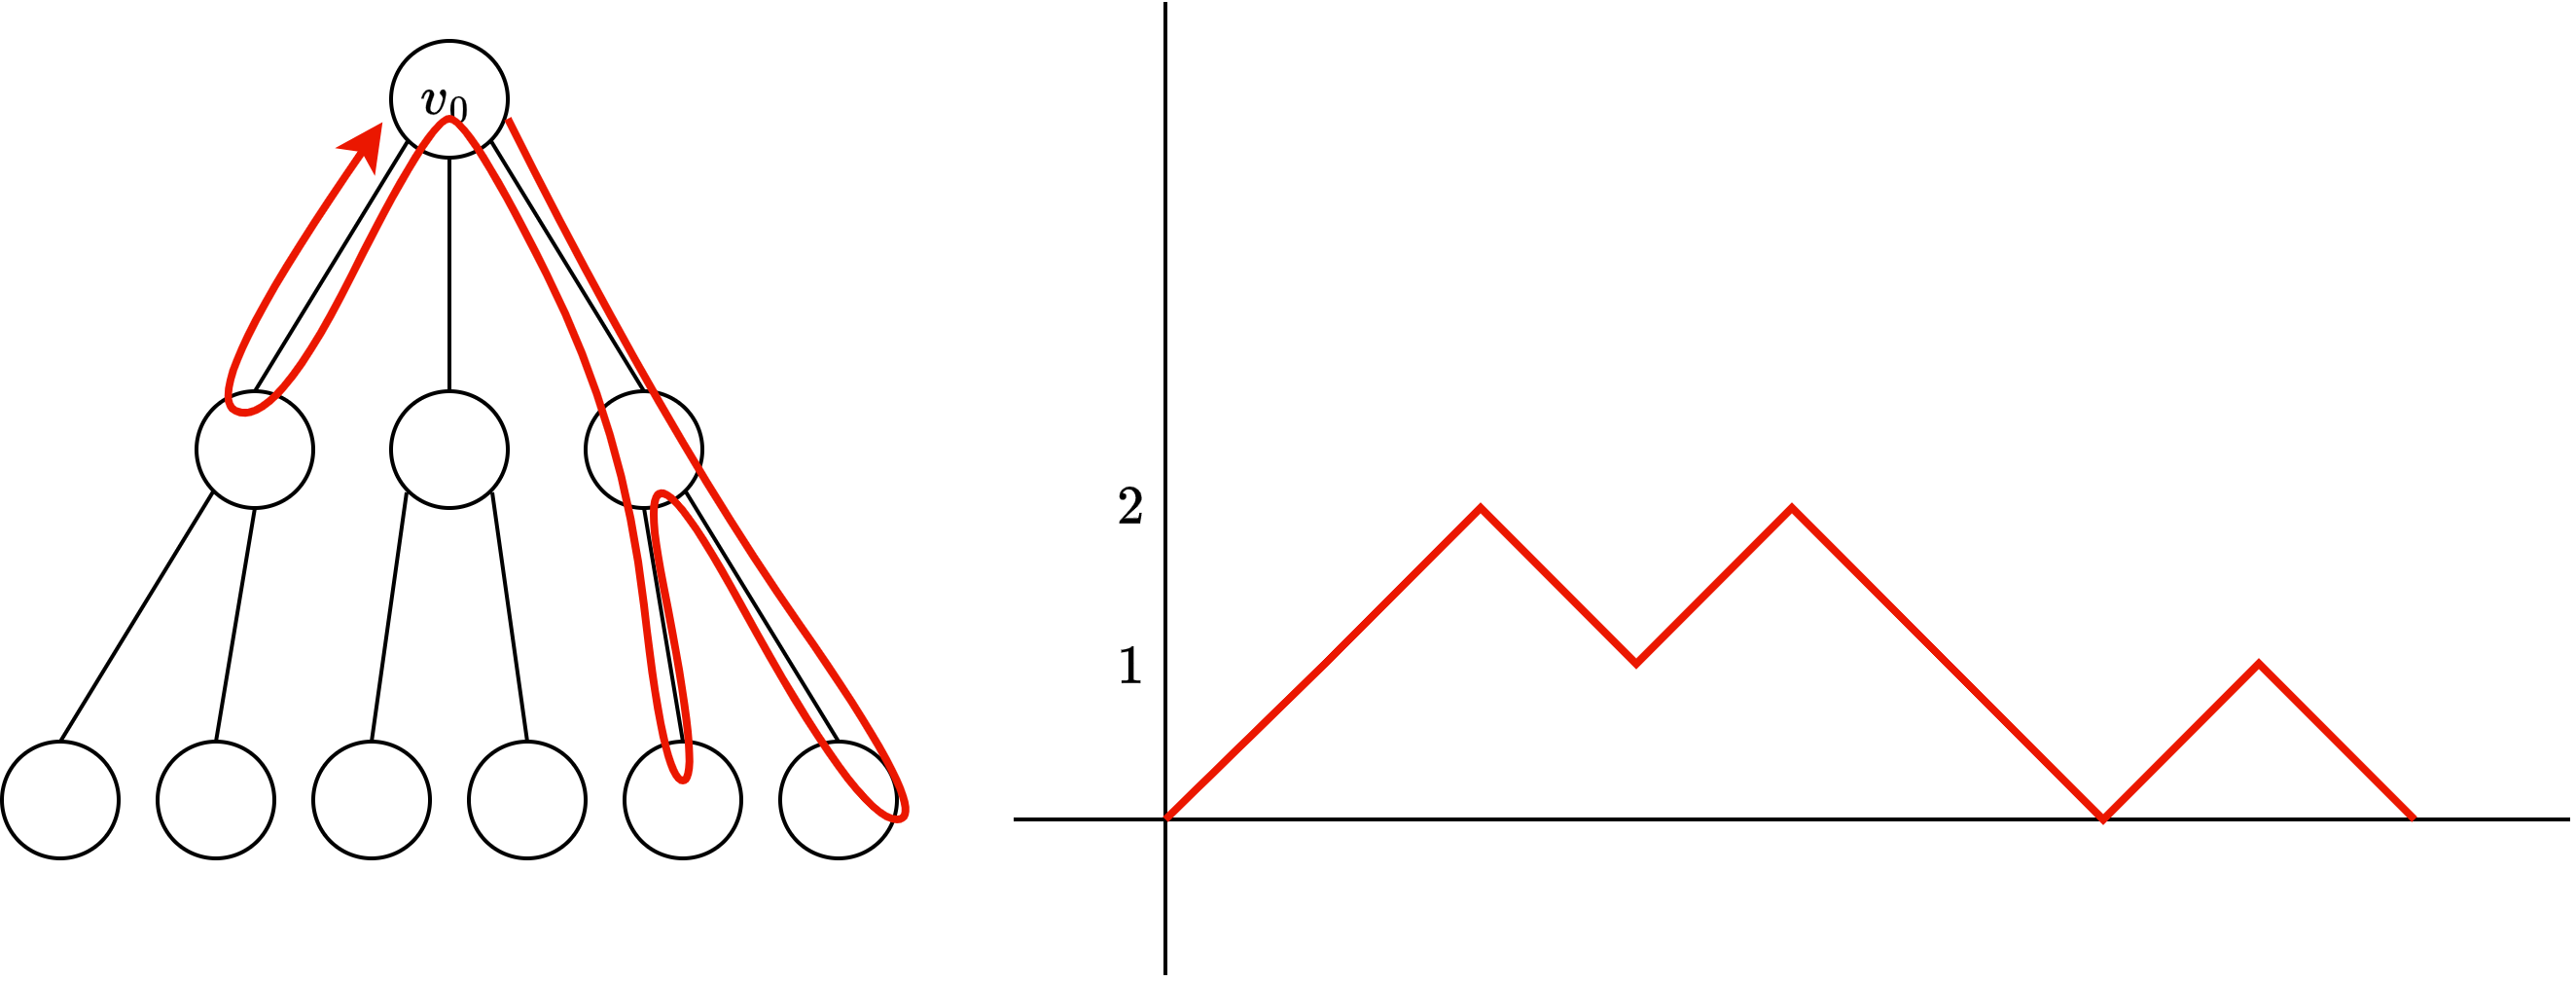
\includegraphics[width=12cm]{images/tree.png}
            \caption{$3$正則木$T$上の長さ$10$の閉路. 親から子への遷移と子から親への遷移を$5$回ずつ行う. 右図は深さ$d_i$の遷移を表す.}
        \end{center}
    \end{figure}

    木$T$において根を始点とする長さ$2k$の閉路$(v_0,\dots,v_{2k})$を考える (ここで$v_0=v_{2k}$).
    各$i$に対して$d_i = \mathrm{depth}(v_i)$とし, 列$(d_0,\dots,d_{2k})$を考える.
    まず$d_0=0$であり, その後は$d_{i+1} \in \cbra{d_i \pm 1}$であり, 常に非負を保ちながら最後に$d_{2k}=0$となる.
    このような列$(d_0,\dots,d_{2k})$の総数はカタラン数と等しく, $\frac{1}{k+1}\binom{2k}{k}$に等しい.
    特に, 各$d_i - d_{i-1}$の符号を見ると$d_0 = d_{2k} = 0$より正と負がそれぞれ$k$個ずつ含まれている.

    次に, 各$(d_1,\dots,d_{2k})$に対して深さの履歴がこれと等しくなるような閉路の個数を考える.
    各$i\ge 2$において, $d_i=d_{i-1}+1$ (すなわち$v_i$が$v_{i-1}$の子である)とき, $v_i$の選び方は少なくとも$d-1$通りある ($v_i$が根であるときは$d$通りあるがこれも下から$d-1$で抑える).
    一方で親に遷移する場合はその遷移先は一意である.
    子への遷移はちょうど$k$回発生するため, 深さの履歴が与えられた$(d_1,\dots,d_{2k})$に等しくなるような閉路の個数は少なくとも$(d-1)^{k}$個存在する.
    従って$t_{2k} = \frac{1}{k+1}\binom{2k}{k} \cdot (d-1)^{k}$を得る.

    後半の主張を証明する.
    $d$-正則グラフ$G$の頂点$u_0$を一つ固定する.
    木$T$の頂点集合を$U$, グラフ$G$の頂点集合を$V$とし,
    $N_T$の定義と同様にグラフ$G$の頂点$v \in V$に対しその$d$個の隣接頂点の集合を$N_G(v)$で表す.
    $G$から$T$への準同型写像$\phi \colon U \to V$を以下のように構成する\footnote{グラフ$G=(V,E)$から$H=(W,F)$への\emph{準同型写像 (homomorphism)}とは, 写像$\phi\colon V\to W$であって$\{u,v\}\in E\Rightarrow \{\phi(u),\phi(v)\}\in F$を満たすものである. ここでは自然に無限グラフに対してこの概念を拡張している.}:
    深さに関して帰納的に定義する.
    \begin{itemize}
        \item まず, $\phi(v_0) = u_0$とする.
              根$v_0$の子$N_T(v_0)$から$N_G(u_0)$への全単射$\phi_0$を任意に一つ選び,
              $\phi\colon N_T(v_0) \ni v' \mapsto \phi_1(v') \in N_T(u_0)$
              によって$N_T(v_0)$における$\phi$を定義する.
        \item $T$における深さ$\ell$以下の全ての頂点に対し$\phi(v)$が定義されているとする. 深さ$\ell$の各頂点$v$に対し, その親を$p$, 子を$c_1,\dots,c_{d-1}$とする. $v$とその親$p$に対しては$u\defeq \phi(v)$, $u_p\defeq \phi(p)\in U$が定義されている. このとき, 全単射$\psi\colon N_T(v)\setminus \{p\} \to N_G(u)\setminus\{u_p\}$を任意に一つ固定し, 各$\phi(c_j)$を$\psi(c_j)\in V$とする.
    \end{itemize}
    このようにして定義された写像$\phi\colon U \to V$は確かに準同型なので
    $T$の閉路$(v_0,\dots,v_{2k})$に対して$(\phi(v_0),\dots,\phi(v_{2k}))$は$G$の閉路になっている.
    さらに, $(\phi(v_0),\dots,\phi(v_{2k}))$の形になっている$G$の閉路が与えられたとき, $v_0$は一意に定まり, 以降の$v_i$は$\phi$の帰納的な定義で用いた全単射の逆写像を用いて順番に復元することができるため, $(v_0,\dots,v_{2k}) \mapsto (\phi(v_0),\dots,\phi(v_{2k}))$は単射である.
    従ってグラフ$G$に含まれるある頂点を始点とした長さ$2k$の閉路の個数は少なくとも$t_{2k}$である.
\end{proof}


\subsection{ラマヌジャングラフ}
漸近的に\cref{thm:Alon Boppana}を達成するグラフを\emph{ラマヌジャングラフ (Ramanujan graph)}という.
\begin{definition}{ラマヌジャングラフ}{Ramanujan graph}
    $d$-正則グラフ$G=(V,E)$は, その単純ランダムウォークの遷移確率行列$P$の第二固有値$\lambda_2$が$\lambda_2 \le 2\sqrt{d-1}$を満たすとき, \emph{ラマヌジャングラフ (Ramanujan graph)}という.
\end{definition}

\cref{thm:Alon Boppana}を達成するグラフ列, すなわち,
次数$d$を固定したときに頂点数が増大していくグラフ列$(G_n)_{n\in\Nat}$であって各$G_n$が$d$-正則ラマヌジャングラフとなるものは存在
するだろうか?
この漸近的に最適な正則エクスパンダーグラフの構成は\citet{LPS88,Mar88}によって独立同時期に初めてその構成が与えられた.
彼らは$d-1$が$4$で割った余りが$1$となる素数であるときに$d$-正則ラマヌジャングラフの列を構成した.
なお, 「ラマヌジャングラフ」という名称は\cite{LPS88}の証明がラマヌジャン予想と呼ばれる予想に依拠しているからである
(「予想」と書いたが当時は既に解決している).
その後, \citet{Mor94}によって次数が素数べき$+1$の形であってもラマヌジャングラフが構成できることが示された.
\begin{theorem}{ラマヌジャングラフの陽な構成}{LPS Ramanujan}
    任意の素数$q$と任意の$k\in\Nat$に対して, 頂点数が発散するある$(q^k+1)$-正則ラマヌジャングラフの列が存在し, 陽に構成できる.
\end{theorem}
%また, \cite{LPS88}とは独立同時期に\citet{Mar88}もラマヌジャングラフの族を構成しているようである
%    (元論文はロシア語で書かれており, 英語に翻訳されたものもあるようなのだが見つけることはできなかった).

\paragraph*{ランダム正則グラフ.}
\citet{LPS88}やその後続研究によりラマヌジャングラフ列については様々な構成方法が知られている.
では, そもそもラマヌジャングラフは何個あるのだろうか?
$n$頂点$d$-正則グラフ全体の集合を$\calG_{n,d}$とし,
$\calG_{n,d}$から一様ランダムに選ばれたグラフ$G\sim\calG_{n,d}$を考える
($nd$は常に偶数とする).
この確率変数をランダム正則グラフという.
ランダム正則グラフは「ほぼ」ラマヌジャングラフであることが知られている
\cite{Friedman_random_regular}.
\begin{theorem}{Friedmanの定理}{random regular graph Ramanujan}
    任意の$d\ge 3$と任意の$\varepsilon > 0$に対し,
    \[ \lim_{n\to\infty}\Pr\sbra*{\lambda(P) \ge \frac{2\sqrt{d-1}}{d} + \varepsilon} = 0. \]
\end{theorem}
すなわち, ほとんど全ての定数次数正則グラフはラマヌジャングラフとほぼ同等のスペクトルを持つ.

\subsection{ジグザグ積による組合せ的な構成}
\begin{definition}{置換積}{replacement product}
    グラフ$G=(V,E)$を$N$頂点$D$-正則グラフとし, グラフ$H=([D],F)$を$[D]$を頂点集合に持つ$D$頂点$d$-正則グラフとする.
    グラフ$G$の各頂点$u\in V$の隣接頂点は$1$から$D$の番号づけが付随していて$N(u)=\{u_1,\dots,u_D\}$とする.

\end{definition}

\section{性質}
エクスパンダーグラフは固有値によって定義されるが, 様々な興味深い性質を持つことが知られている.
ここではグラフ理論的な性質と擬似ランダム性について紹介する.
%


\subsection{擬似ランダム性(*)} \label{sec:expander pseudorandom}
この節は高次元エクスパンダーの本筋から少し外れるが,
エクスパンダーグラフの重要であることの理由の一つとしてその擬似ランダム性について概説する.

加法的組合せ論や計算量理論では\emph{擬似ランダム性 (pseudorandomness)}と呼ばれる概念が非常に重要な役割を果たしている.
\begin{definition}{分布の擬似ランダム性}{pseudorandomness}
    有限集合$\Omega$上のある分布$\mu$と関数族$\mathcal{F} \subseteq \{f\colon \Omega \to \binset\}$を考える.
    分布$\mu$は,
    任意の$f\in \mathcal{F}$に対して
    \[ \abs*{\E_{x\sim \mu} [f(x)] - \E_{y\sim U_{\Omega}}[f(y)]} \le \varepsilon\]
    を満たすとき, \emph{$\mathcal{F}$に対して$\varepsilon$-擬似ランダムである}という (ここで, $y\sim U_\Omega$とは$\Omega$上一様ランダムに$y$が選ばれたことを意味する).
\end{definition}
直感的には, 分布が擬似ランダムであるとは, その分布が任意の$f\in \mathcal{F}$を使っても一様分布と\emph{識別できない (indistinguishable)}ことを意味する.
例えば全変動距離に関する\cref{prop:dtv}では, $\mathcal{F}$を$V$上の二値関数全体 (すなわち任意の$V$の部分集合)の族としたときの識別不可能性のパラメータ$\varepsilon$が全変動距離で与えられることを意味する.
すなわち$\mu$は常に$\dtv(\mu,U_{\Omega}))$-擬似ランダムである.
関数クラス$\mathcal{F}$をより制限したときにパラメータ$\varepsilon$がどこまで小さくなるかに興味がある.

組合せ論では$\mathcal{F}$としてある特殊な関数クラスを仮定することによって\emph{組合せ論的擬似ランダム性}を定義する.
例えばグラフ理論や加法的組合せ論のコーナーストーンの一つと呼ばれるSzemerédiの正則化補題と呼ばれる結果は, 非常に大雑把に言えば
任意の密なグラフが定数個の擬似ランダムな二部グラフと疎な部分に分解できることを主張する定理である.
組合せ論的擬似ランダムネスの概念は特に加法的組合せ論において非常な協力な道具となっており,
Green--Taoの定理の証明においても重要な役割を果たしている
(驚くべきことに, 識別不可能性の枠組みでGreen--Taoの定理の証明を理解してそれを学習理論におけるブースティングの証明に応用するという研究もなされている!).

計算量理論では$\mathcal{F}$を「効率的なアルゴリズムの全体」や「素子数の少ない論理回路の全体」とすることで\emph{計算量的擬似ランダム性}を定義できる.
任意の効率的なアルゴリズムに対して一様ランダムな文字列と識別できないということは, その分布に従って生成されたメッセージを盗み見てもそこから得られる情報が何もない (ランダムな文字列を見てるのと同じ) であることから, 計算量的擬似ランダム性は暗号の計算量的安全性の定義の根幹をなすことがわかる.

エクスパンダーグラフの組合せ論的擬似ランダム性を説明する.
正則$\lambda$-エクスパンダー$G=(V,E)$を考える.
集合$\Omega=V\times V$上の分布$\mu = \mu_G$として
一様ランダムな辺$\{u,v\}\in E$を選び, $(u,v)$もしくは$(v,u)$どちらかを等確率で選んだ時の頂点対の分布とする.
すなわち,
\begin{align}
    \Pr_{(u,v)\sim \mu}\sbra*{ (u,v) = (s,t)} = \frac{\indicator{\{s,t\}\in E}}{2\abs{E}} = \frac{\indicator{\{s,t\}\in E}}{nd} \label{eq:expander mu}
\end{align}
とする.
関数族$\mathcal{F}$を
\begin{align}
    \mathcal{F} = \cbra*{ f_{S,T} \colon (s,t) \mapsto \indicator{s\in S,t\in T} \colon S,T\subseteq V}  \label{eq:expander F}
\end{align}
で定める.

以下の結果は\citet{AC88}によるものである.
%
\begin{lemma}{エクスパンダー混交補題}{expander mixing lemma}
    任意の頂点部分集合$S,T\subseteq V$に対して,
    $e(S,T) = \sum_{s\in S,t\in T} \indicator{\{s,t\} \in E}$を$S,T$間の辺の本数($S\cap T$内の辺は2回数える)とすると,
    \[
        \abs*{e(S,T) - \frac{d}{n}|S||T|} \le d\lambda\sqrt{|S||T|\rbra*{1-\frac{|S|}{n}}\rbra*{1-\frac{|T|}{n}}}.
    \]
    同様に, $G$が片側$\lambda$-エクスパンダーならば,
    \[
        e(S,T) - \frac{d}{n}|S||T| \le d\lambda\sqrt{|S||T|\rbra*{1-\frac{|S|}{n}}\rbra*{1-\frac{|T|}{n}}}.
    \]
\end{lemma}

\begin{corollary}{擬似ランダム性}{pseudorandomness expander}
    グラフ$G$が$n$頂点$d$-正則$\lambda$-エクスパンダーであるとき, \cref{eq:expander mu}で定義された分布$\mu$は\cref{eq:expander F}で定義された関数族$\mathcal{F}$に関して$\frac{\lambda}{4}$-擬似ランダムである.
\end{corollary}
%
グラフ$G$の隣接行列$A$を考えるとイメージしやすい.
この行列は全部で$nd$個の$1$を持っているため, 全成分の中で$1$の密度は$\frac{d}{n}$である.
ここで, 部分集合$S,T\subseteq V$に対して$A$の$S\times T$で定まる部分行列$A_{S,T}$を考える.
この行列に含まれる$1$の個数($e(S,T)$に等しい)は, $\frac{d}{n}\cdot |S||T|$に近い値となっている (\cref{fig:EML}).
\begin{figure}[htbp]
    \begin{center}
        \includegraphics[width=6cm]{images/EML.pdf}
        \caption{正則グラフの隣接行列$A$を考える. このグラフがエクスパンダーならば, 頂点部分集合$S,T\subseteq V$で指定される長方形内に含まれる$1$の密度は行列全体の$1$の密度に近い値をとる. \label{fig:EML}}
    \end{center}
\end{figure}
%
\begin{proof}[\cref{lem:expander mixing lemma}の証明.]
    グラフ$G$上の単純ランダムウォーク$P$を考える.
    部分集合$S,T\subseteq V$に対し
    関数$f=\delta_S,g=\delta_T$として
    \cref{cor:general expander mixing lemma}を適用すると
    \begin{align*}
         & \piprod{f,Pg} = \frac{e(S,T)}{nd},               \\
         & \Epi f = \frac{|S|}{n},                          \\
         & \Epi [Pg] = \Epi g = \frac{|T|}{n},              \\
         & \Varpi f = \frac{|S|}{n}\rbra*{1-\frac{|S|}{n}}, \\
         & \Varpi g = \frac{|T|}{n}\rbra*{1-\frac{|T|}{n}}
    \end{align*}
    より整理すると主張を得る.

    グラフ$G$が片側エクスパンダーである場合は\cref{cor:general expander mixing lemma}の代わりに\cref{lem:one side EML}を適用すればよい.
\end{proof}
\begin{exercise}{}{check}
    \cref{lem:expander mixing lemma}の証明で表した五つの等式を実際に確認せよ.
\end{exercise}
\begin{proof}[\textbf{解答}]
    $f$についての等式を示せば, $S$を$T$に置き換えるだけで$g$に関する等式が得られるので$f$についてのみ示す.
    \begin{align*} 
         \piprod{f,Pg} &= \sum_{u,v\in V} \pi(u)f(u)P(u,v)g(v) \\
         &= \frac{1}{n}\sum_{u\in S,v\in T} \frac{\indicator{\{u,v\}\in E}}{d} \\
         &= \frac{e(S,T)}{nd}.
    \end{align*}
    \begin{align*} 
         \Epi f &= \sum_{u\in V} \pi(u)f(u) \\
         &= \sum_{u\in S}\frac{1}{n}\\
         &= \frac{|S|}{n}.
    \end{align*}
    $\Varpi f$について, $f^2=f$より
    \begin{align*} 
         \Varpi f &=  \Epi[f^2] - \Epi[f]^2 \\
         &= \frac{|S|}{n} - \frac{|S|^2}{n^2} \\
         &= \frac{|S|}{n}\rbra*{ 1 - \frac{|S|}{n} }.
    \end{align*}    
\end{proof}

「エクスパンダー混交補題」と言うと聞こえが良いが, \cref{cor:general expander mixing lemma}を見るとその実は単なるCauchy--Schwarzの不等式とレイリー商の議論を適用しただけであることがわかる.

エクスパンダー混交補題の応用として, エクスパンダーグラフ上のランダムウォークはずっと同じ頂点部分集合にとどまらないことを示せる.
\begin{proposition}{}{expander walk hitting}
    グラフ$G=(V,E)$を$n$頂点$d$-正則片側$\lambda$-エクスパンダーとし,
    $(X_t)_{t\ge 0}$を$G$上の単純ランダムウォークで初期頂点$X_0$が$V$上一様ランダムに選ばれたものとする.
    任意の$\ell\in\Nat$と頂点部分集合$B\subseteq V$に対し, $\mu = \frac{|B|}{n}$とすると, 以下が成り立つ:
    \[
        \Pr\sbra*{\text{全ての$t=0,\dots,\ell$に対し}X_t \in B} \le \rbra*{ \mu + \lambda(1-\mu)}^\ell.
    \]
\end{proposition}
\begin{proof}
    $\ell\ge 0$に対し$\mathcal{E}_\ell$を「全ての$t=0,\dots,\ell$に対し$X_t\in B$」という事象とする.
    初期頂点$X_0$が定常分布($=$一様分布)に従って選ばれているため, 各$t$に対し$X_t$の周辺分布もまた一様分布である.
    特に, \cref{lem:expander mixing lemma}より, 任意の$t\ge 0$に対し
    \begin{align}
        \Pr\sbra*{ X_{t+1} \in B \text{ かつ }X_t \in B} &= \frac{e(B,B)}{nd} \nonumber\\
        &\le \mu^2 + \lambda\mu(1-\mu) \label{eq:eml bound}
    \end{align}
    を得る.
    従って
    \begin{align*}
        \Pr\sbra*{\mathcal{E}_\ell} &= \Pr\sbra*{ X_\ell \in B \condition \mathcal{E}_{\ell-1} }\cdot \Pr\sbra*{\mathcal{E}_{\ell-1}} \\
        &= \Pr\sbra*{X_\ell \in B \condition X_{\ell-1} \in B}\cdot \Pr\sbra*{\mathcal{E}_{\ell-1}} \\
        &= \frac{\Pr\sbra*{ X_{t+1} \in B \text{ かつ }X_t \in B}}{\mu} \cdot \Pr\sbra*{\mathcal{E}_{\ell-1}} \\
        &\le \rbra*{\mu + \lambda(1-\mu)}\cdot \Pr\sbra*{\mathcal{E}_{\ell-1}} & & \text{$\because$\cref{eq:eml bound}} \\
        &\dots \\
        &\le \rbra*{\mu + \lambda(1-\mu)}^\ell\cdot \Pr[\mathcal{E}_0] \\
        &\le \rbra*{\mu + \lambda(1-\mu)}^\ell
    \end{align*}
    より主張を得る.
\end{proof}

\subsection{グラフ理論的な性質}
本講義とは直接の関係はないが,
エクスパンダーグラフはグラフ理論的に非常に興味深い多くの性質を有するため,
いくつかを簡単に紹介する.
本節では主に正則グラフに対する組合せ論的な性質について述べる.

\begin{proposition}{低直径性}{small diameter}
    $n$頂点$(1-\gamma)$-エクスパンダーの直径は高々$\ceil*{\frac{12\log n}{\gamma}}$.
\end{proposition}
\begin{proof}
    二頂点$u,v$を任意に固定し,
    $u$を始点とした単純ランダムウォーク$(X_t)_{t\ge 0}$を考える.
    定常分布$\pi$は$\pimin \ge \frac{1}{2|E|} \ge n^{-2}$を満たす.
    従って\cref{lem:mixing time and spectral gap}を$\varepsilon=n^{-2}/2$に対して適用すると,
    \[
        \tmix(n^{-10}) \le \frac{4\log n}{\gamma}.
    \]
    $\ell=\ceil*{\frac{4\log n}{\gamma}}$とする.
    混交時間の定義(\cref{def:mixing time})より$\dtv(X_{\ell}, \pi) \le n^{-2}/2$であり, 任意の頂点$v\in V$に対し
    $\pi(v) \ge n^{-2}$なので,
    \[
        \Pr[X_\ell = v] \ge \pi(v) - \dtv(X_\ell,\pi) >0
    \]
    すなわち, 正の確率で$X_\ell = v$となるので, 特に$\dist(u,v) \le \ell$を得る.
    これが任意の$u,v$に対して成り立つので主張を得る.
\end{proof}
%\todo[inline]{Cheeger, chromatic number, diameter}

グラフ$G = (V,E)$の頂点部分集合$S\subseteq V$は, $e(S,S)=0$, すなわち$S$内に辺が存在しないとき\emph{独立点集合 (independent set)}という.
独立点集合のうち最大要素数を$\alpha(G)$と表す.
\begin{proposition}{}{independence number}
    任意の$n$頂点正則$\lambda$-エクスパンダー$G$は, $\alpha(G) \le \frac{\lambda}{1+\lambda}n$を満たす.
\end{proposition}
\begin{proof}
    独立点集合$S\subseteq V$をとり, $|S|= \alpha n$とする.
    \cref{lem:expander mixing lemma}より,
    \[
        0 = e(S,S) \ge  d \alpha^2 n - d\lambda \alpha(1-\alpha) n = d\alpha n (\alpha - \lambda(1-\alpha)).
    \]
    すなわち$\alpha - \lambda(1-\alpha) \le 0$となり, これを解くと$\alpha\le \frac{\lambda}{1+\lambda}$を得る.
\end{proof}

他の特に重要な性質として, \emph{Cheegerの不等式}\cite{Cheeger70}が知られている.
ここでは証明は与えずに結果だけ述べる.
%
\begin{definition}{}{edge expansion}
    $d$-正則グラフ$G=(V,E)$とその頂点部分集合$S\subseteq V$に対し,
    $S$の\emph{辺膨張率 (edge expansion)} $\phi(S)$を
    \[
        \phi(S) = \frac{e(S,V\setminus S)}{d\abs{S}}
    \]
    で定める. グラフ$G$の辺膨張率 (または\emph{Cheeger定数}) $\phi(G)$を
    \[
        \phi(G) = \min_{0 \le |S| \le |V|/2} \phi(S)
    \]
    とする.
\end{definition}
$\phi(S)$の分母の値$d|S|  =\sum_{v\in S}\deg(v)$は$S$に接続している辺の総数に等しい ($S$内部をつなぐ辺は2回カウントされている).
分子の$e(S,V\setminus S)$はこれらのうち, $S$の外側($V\setminus S$)に接続している辺を数えている.
従って, $\phi(S)$が大きいということは, 多くの割合の辺が$S$の外側に接続していることを意味する.
\begin{theorem}{Cheegerの不等式}{Cheeger inequality}
    任意の正則片側$\lambda$-エクスパンダーグラフは
    \[
        \frac{1-\lambda}{2} \le \phi(G) \le \sqrt{2(1-\lambda)}
    \]
    を満たす.
\end{theorem}


\section{エクスパンダーグラフの応用} \label{sec:expander graph application}
グラフのエクスパンダー性は組合せ論的な興味だけでなく,
理論計算機科学において多くの定理の証明の道具として非常に重要な役割を果たしている.
ここではその一端を軽く紹介する.
より詳細の議論は\cite{HLW06}を参照されたい.
%
\subsection{脱乱択化}
乱択は計算能力を真に向上させるかという問いは計算量理論において今なお重要な未解決問題であり,
暗号の計算量理論的安全性などにも応用される.
この分野の中心的なリーダーの一人Avi Wigdersonは2021年にAbel賞, 2023年にTuring賞を受賞している.
興味深いことに計算量理論では「乱択計算を決定的に模倣できる」\footnote{この文は非常に大雑把であり, 考える問題設定に大きく依存する. 専門用語を使うと「確率的多項式時間チューリング機械で解ける判定問題は決定的多項式時間で解けるか?」という未解決問題($\mathsf{P}=\mathsf{BPP}$予想)は真であろうと専門家に信じられている.}という見解が主流を占めている.
すなわち, 乱択計算に用いるコイントスをなくせるというのである!
ここではエクスパンダーグラフを使って乱択計算に用いるコイントスの「回数」を減らす手法\cite{AKS87}を紹介する.

本来ならば乱択計算を定義するためにチューリング機械の定義から始める必要があるのだが,
それらは本講義のトピックから大きく逸脱してしまうので,
ここでは大きく簡略化した次の設定を考えよう:
集合$\{0,1\}^n$の各元に$0$または$1$のどちらかの数字が割り当てられており, $1$が割り当てられたものを「あたり」とみなしたくじ引きを行う.
「あたり」の個数は少なくとも$\varepsilon\cdot 2^n$個ある.
確率$1/2$以上で「あたり」を引く方法のうち, ランダムネスをできるだけ少なくしたい.



愚直に考えると, 適当なパラメータ$k$に対し,
独立一様ランダムに$k$個の文字列$r_1,\dots,r_k\sim\binset^n$を選び, その中に「あたり」があるかどうかを確認すればよい.
これらの中に「あたり」が一つ以上含まれる確率は$1-(1-\varepsilon)^k \ge 1-\exp(-k\varepsilon)$なので, 成功確率$1/2$を達成するには$k=O(1/\varepsilon)$とすればよい.
各$r_i$を選ぶにはそれぞれで$n$ビットのランダムネスを要するので, 全体で$kn = O(n/\varepsilon)$ビットのランダムネスが必要である.

\begin{proposition}{}{expander derandomize}
    $n + O\rbra*{1/\varepsilon}$ビットのランダムネスを用いて確率$1/2$以上で「あたり」を引く方法がある.
\end{proposition}
\begin{proof}[\textbf{証明の概要.}]
    頂点数$2^n$の$8$-正則$0.9$-エクスパンダーグラフ$G=(V,E)$を\cref{thm:Margulis construction}を用いて決定的に構成し, 適当な全単射を用いて$V$を$\binset^n$と同一視する (ここで用いる全単射は何でもよい).
    あとで定まる適切なパラメータ$\ell\in\Nat$に対し,
    初期頂点を一様ランダムにした
    $G$上の$\ell$ステップの単純ランダムウォーク$(X_t)_{t=0,\dots,\ell}$を考え,
    訪問した頂点$X_0,\dots,X_\ell$の中に「あたり」があるかどうかを調べる.
    初期頂点の選択で$n$ビットのランダムネスを用いるが,
    グラフ$G$は$8$-正則グラフなのでランダムウォークの各遷移では$\log_2 8=3$ビットのランダムネスを使用する.
    従って, この方法で用いるランダムネスは全体で$n + 3\ell$ビットである.

    「あたり」以外の頂点からなる集合を$B$とすると, $\frac{|B|}{2^n} = 1-\varepsilon$なので,
    $\mu = 1-\varepsilon, \lambda=0.9$として\cref{prop:expander walk hitting}を適用すると,
    $\ell=10/\varepsilon$に対して
    少なくとも確率$1-(1-0.1\varepsilon)^\ell \ge 1-\e^{-1} \ge 1/2$で
    ランダムウォークは「あたり」の頂点を一回以上は訪問する.
    すなわち確率$1/2$以上でこの方法は「あたり」を引く.
\end{proof}

乱択計算の文脈では, 一回のくじ引きが乱択計算のシミュレーションに対応しており,
「あたり」を引くということはその乱択計算が正しい計算結果を出力したことを意味する.
独立なランダムネスを用いて繰り返すとその繰り返し回数に比例したランダムネスを要するが,
独立性の代わりにランダムウォークのエクスパンダー性を用いれば, 要するランダムネスの量を減らせるのである.


\subsection{誤り訂正符号} \label{sec:error correcting code}
\emph{誤り訂正符号(error-correcting code)}または単に\emph{符号(code)}とは文字列に冗長性を持たせることでノイズに対する頑健性を与える手法である.
数学的には符号はビット列の集合$\Code\subseteq\mathbb{F}_2^n$であり, その元$f\in\Code$を\emph{符号語(codeword)}と呼ぶ\footnote{文脈によってはビット列の代わりに有限集合$\Sigma$に対して$\Code\subseteq\Sigma^n$を符号と定義することもある. 実際には計算機上では$\Sigma$の元を$\lceil\log_2 |\Sigma|\rceil$ ビットで表すため$\Sigma=\mathbb{F}_2$とすることが多い.}.
ここで$n$を符号$\Code$の\emph{符号長(code length}と呼ぶ.
符号には, 任意の相異なる二つの符号語が互いにハミング距離の意味で離れていることが望まれる.
形式的には, 正規化されたハミング距離$\dist(f,g)=n^{-1}\sum_{i\in[n]}\indicator{f(i)\neq g(i)}=\Pr_{i\sim[n]}[f(i)\neq g(i)]$を考え, $\min_{f\neq g\in\Code}\dist(f,g)$を符号$\mathcal{C}$の\emph{距離(distance)}という.
文字列$f\in\mathbb{F}_2^n$と$\Code\subseteq\mathbb{F}_2^n$に対して$\dist(f,\Code)=\min_{w\in\Code}\dist(f,w)$
を$f$の$\Code$への距離とする.


符号$\Code\subseteq\mathbb{F}_2^n$が線形部分空間となるとき, 符号$\Code$を\emph{線形符号(linear code)}と呼ぶ.
文脈によっては線形符号のことを単に符号と呼ぶこともあり,
本講義も以降は特に断りのない限りこの慣習に従う.
すなわち符号と言えばそれは線形部分空間を意味する.
符号長$n$, ランク$k$の線形符号に対し,
$k/n$をその符号の\emph{レート(rate)}と呼ぶ.
直感的には符号のレートはその符号が空間$\mathbb{F}_2^n$内でどれほど密に充填しているかを表すため,
符号のレートと距離にはトレードオフがある.
線形符号$\Code$の距離は最小ハミング重みを持つ非ゼロの符号語によって与えられることに注意されたい.

ここでは, ケイリーグラフ (\cref{def:Cayley graph}) を用いて構成される符号を紹介する.
\begin{definition}{ケイリーエクスパンダー符号}{Cayley expander code}
    ケイリーグラフ$\Cay(A,G)=(V,E)$と符号$\Code_A\subseteq\mathbb{F}_2^A$を考える.
    頂点$g\in V$と関数$f\colon E \to \mathbb{F}_2$に対し, $f_g=(f(\{g,ag\}))_{a\in A}\in \mathbb{F}_2^A$と定める.
    符号$\Code_A\subseteq \mathbb{F}_2^A$に対して
    \begin{align*}
        \Code(A,G,\Code_A)=\{f\in\mathbb{F}_2^E\colon \forall g\in V, f_g \in \Code_A\}
    \end{align*}
    を\emph{ケイリーエクスパンダー符号}と呼ぶ.
\end{definition}
一般の(ケイリーグラフとは限らない)正則エクスパンダーグラフを用いて定義される\emph{エクスパンダー符号 (expander code)}が有名だが, 定義の簡潔さを優先してあえてケイリーグラフに限定したエクスパンダー符号を紹介した.
もし仮に$A$を生成系とするケイリーグラフの列$(\Cay(A,G_n))_{n\in\Nat}$と
レートと距離の良い性質をもつ一つの符号$\Code_A$があったとしよう.
すると, この一つの符号から符号の列$(\Code_n)_{n\in\Nat} \defeq (\Code(A,G_n,\Code_A))_{n\in\Nat}$を構成できる.

さらに興味深いことに, 構成に用いたケイリーグラフがエクスパンダー性を持つならば
元の符号$\Code_A$のレートと距離の性質を符号列$(\Code_n)$も受け継ぐ.
%
\begin{lemma}{}{expander code rate}
    $\Code_A$のレートが$r_A$ならば
    $\Code(A,G,\Code_A)$のレートは少なくとも$2r_A-1$である.
\end{lemma}
\begin{proof}
    符号$\Code_A\subseteq\F_2^A$のレートが$r_A$なので,
    その任意の符号語$f_0\in \Code_A$は$|A|(1-r_A)$個の線形制約を満たす.
    ケイリーエクスパンダー符号$\Code(A,G,\Code_A)$の符号語$f$は,
    全ての頂点$g\in G$に対して$f_g$が$\abs{A}(1-r_A)$個の線形制約を満たしているので,
    $f$は高々$|G||A|(1-r_A)$個の線形制約を満たしている.
    つまり$f$の自由度は少なくとも$|E|-|G||A|(1-r_A)=|E|(1-2(1-r_A))$なので,
    $\Code(A,G,\Code_A)$のレートは少なくとも$1-2(1-r_A)=2r_A-1$となる.
\end{proof}
%
\begin{lemma}{}{expander code distance}
    符号$\Code_A$の距離が$\delta_A$, ケイリーグラフ$\Cay(A,G)$が$\lambda$-エクスパンダーならば,
    ケイリーエクスパンダー符号$\Code(A,G,\Code_A)$の距離は少なくとも$\delta_A(\delta_A-\lambda)$である.
\end{lemma}
証明にはエクスパンダー混交補題からすぐに従う以下の系を用いる:
\begin{corollary}{}{EML}
    $d$-正則な$\lambda$-エクスパンダー$G=(V,E)$の頂点部分集合$S\subseteq V$が$e(S,S)\geq cd|S|$を満たす(言い換えると, 誘導部分グラフ$G[S]$の平均次数が$cd$以上)ならば, $|S|\geq (c-\lambda)n$を満たす.
\end{corollary}
%

\begin{proof}[\cref{cor:EML}の証明.]
    $S=T$として\cref{lem:expander mixing lemma}を適用すると
    \begin{align*}
        cd|S| \leq e(S,S) \leq \frac{d}{|V|}|S|^2+\lambda d |S|.
    \end{align*}
    これを解くと$|S|\geq (c-\lambda)n$を得る.
\end{proof}
%
\begin{proof}[\cref{lem:expander code distance}の証明.]
    任意の非ゼロの符号語$f\in\Code(A,G,\Code_A)$が少なくとも$\delta_A(\delta_A-\lambda)|E|$個の$1$を持つことを言えばよい.
    符号語$f\neq 0$に対し, $F=\{e\in E\colon f(e)=1\}$とし, $S=\bigcup_{e\in F}e$を$F$の辺と接続している頂点の全体とする(辺$e$を要素数$2$の頂点部分集合として見ている).
    $|F|\geq\delta_A(\delta_A-\lambda)|E|$を示せばよい.

    $\Code_A$の距離の条件より,
    各$g\in S$に対して$f_g\in\F_2^A$は少なくとも$\delta_A|A|$本の辺が接続している.
    すなわち, $\Cay(A,G)$の部分グラフ$(S,F)$の最小次数は$\delta_A|A|$を満たすので$|F|\geq \frac{\delta_A |A|}{2}|S|$.
    誘導部分グラフ$G[S]$は$(S,F)$を部分グラフとして含むので$e(S,S)\geq 2|F|$.
    さらに$(S,F)$に対する握手補題より
    \begin{align*}
        e(S,S)\geq 2|F|\geq \delta_A|A||L|.
    \end{align*}
%
    \Cref{cor:EML}より$|S|\geq (\delta_A-\lambda)|G|$なので,
    $|F|\geq \frac{\delta_A|A|}{2}|S|\geq \delta_A(\delta_A-\lambda)\frac{|G||A|}{2}=\delta_A(\delta_A-\lambda)|E|$を得る.
\end{proof}

%\todo[inline]{下論文の二部エクスパンダーに基づく定義との比較}


\chapter{高次元エクスパンダー概論} \label{chap:HDX}
高次元エクスパンダーとはグラフのエクスパンダー性を単体複体に拡張した概念である.
単体複体上では, 大域的なランダムウォークと局所的なランダムウォークの二つのタイプのランダムウォークを自然に考えることができ, これらに基づいてそれぞれ大域的なエクスパンダー性と局所的なエクスパンダー性の概念が定義できる.
端的に述べると高次元エクスパンダーの理論はこれら二つの概念がほぼ等価であることを明らかにしており, これは単体複体における局所大域原理\footnote{ここでは局所大域原理(local-global principle)は局所的な情報が大域的な情報を導くという現象の総称として用いるが, もともとは整数論において不定方程式の解の存在性に関するハッセの原理と呼ばれる現象を指す.}を体現しているといえる.

本チャプターではまず単体複体とその上でのランダムウォークを定義し,
これに基づいて高次元エクスパンダーの定義と重要な性質を紹介する.

本講義資料は第一線で活躍している海外の研究者らの講義資料も参考にした \cite{LapChiLau_Lecture,Gharan_Lecture,MaxHopkins_Lecture}.

\section{定義} \label{sec:define simplicial complex}
まずは単体複体に関する基礎的な用語を定義していく.
文脈によっては単体複体は多面体などを貼り合わせた幾何的な図形を指すこともあるが,
本講義ではいわゆる抽象的単体複体を単体複体とする.
\begin{figure}
    \begin{center}
    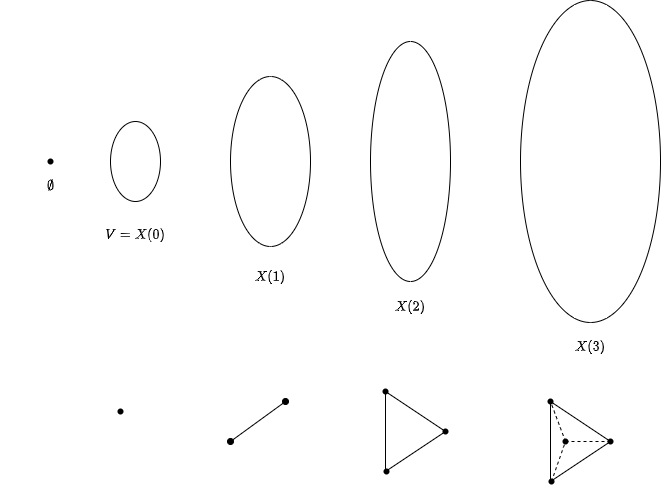
\includegraphics[width=12cm]{images/face.png}
    \caption{各面の図形的な意味合い. \label{fig:face}}
    \end{center}
\end{figure}

\begin{definition}{単体複体}{simplicial complex}
有限集合$V$と$V$の部分集合族$\F\subseteq 2^V$であって部分集合で閉じているもの(すなわち, $\sigma\subseteq \tau \in \F \Rightarrow \sigma\in \F$)の組$X=(V,\F)$を\emph{単体複体 (simplicial complex)}という.
\begin{itemize}
\item 集合族$\F$の元を\emph{面 (face)}と呼び,
面$\sigma \in \F$の\emph{次元 (dimension)}を$\dim \sigma = \abs{\sigma} - 1$とする\footnote{特に, 空集合$\emptyset \in \F$の次元は$-1$である.}.
単体複体$X$の次元を$\dim X = \max\cbra{\dim \sigma \colon \sigma \in \F}$とする.

\item 次元$d$の単体複体$X$は(包含関係に関して)極大な面の次元が全て$d$に等しいとき, \emph{純粋 (pure)}であるという.

\item 整数$-1 \le k \le \dim X$に対し$X(k) = \cbra*{\sigma \in \F\colon \dim \sigma = k }$とする.
特に断りのない限り, $X(0)=V$を仮定する
(そうでなければ$V$として$V=X(0)$とした単体複体を考える).

\item 純粋な$d$-次元単体複体$X$に, $d$次元の面全体$X(d)$上の何らかの分布$\pi \in [0,1]^{X(d)}$が付随している場合, $X$を\emph{重み付き単体複体 (weighted simplicial complex)} (もしくは$\pi$で重みつけられた単体複体)と呼ぶ.
\end{itemize}
以後, 単体複体といった場合, 暗に重み付き単体複体を考え, 最大次の面の重みを$\pi$で表す.
\end{definition}
面の次元の概念は単体複体の幾何的な表現に由来する.
このイメージになぞらえて,
次元$0$の面を\emph{頂点 (vertex)}, 次元$1$の面を\emph{辺 (edge)}と呼ぶことがある.

記法の簡単のため, 面$\sigma$と頂点$u\in V$に対し$\sigma \setminus \{u\}$を簡略化して$\sigma \setminus u$と書くこともある.

\paragraph*{例1.}
グラフ$G=(V,E)$に対し, 空集合, $V$, $E$からなる部分集合族
$\F = \{\emptyset\} \cup \cbra*{\{v\}\colon v \in V} \cup E$考えると,
$(V,\F)$は単体複体である.

\paragraph*{例2.}
有限集合$V$に対し,
\begin{align}
    \F = \binom{V}{\le k} \defeq \cbra*{ \sigma \subseteq V \colon |\sigma|\le k} \label{eq:uniform matroid}
\end{align}
としたとき, $(V,\mathcal{F})$は純粋な$(k+1)$-次元の単体複体である.

\paragraph*{例3.}
閉路を含まないグラフを\emph{森 (forest)}といい, 連結な森を\emph{木 (tree)}という.
連結グラフ$G$の部分グラフであって木であるものを\emph{全域木 (spanning tree)}という (cf. \cref{def:graph}).
グラフ$G=(V,E)$に対し,
森であるような部分グラフの辺集合からなる集合族$\F\subseteq 2^E$は単体複体である.
すなわち,
\begin{align}
    \F = \cbra*{ F \subseteq E \colon \text{部分グラフ$(V,F)$は森}} \label{eq:graphic matroid}
\end{align}
に対して$(E,\F)$は単体複体である.
簡単のため$G$を連結グラフであるとすると, $(E,\F)$の極大面は$G$の全域木に対応し, その次元は$n-2$に等しい.
すなわち$(E,\F)$は純粋な$(n-2)$-次元単体複体である.

なお, グラフ$G$が連結でない場合, 異なる連結成分に属する二頂点$u,v$を縮約し一つの頂点として扱うことによって単体複体$(E,\F)$を変えないまま元のグラフの連結成分を減らすことができるので, 連結性を仮定しても一般性を失わない.

\paragraph*{例4.}
ベクトル$\vec{a_1},\dots,\vec{a_n} \in \Real^m$を考える.
集合$V=\{1,\dots,n\}$の部分集合族であって, 線形独立な行ベクトル集合のインデックスとなるものの全体を$\F$とする.
すなわち
\begin{align}
    \F = \cbra*{ I \subseteq V\colon (\vec{a_i})_{i\in I}\text{は線形独立}} \label{eq:linear matroid}
\end{align}
とすると, $(V,\F)$は純粋な単体複体である.

\paragraph*{例5.}
部集合$L,R$を持つ二部グラフ$G=(V,E)$を考える.
辺部分集合$M\subseteq E$は, 部分グラフ$(V,M)$の全ての頂点の次数が高々$1$であるとき\emph{マッチング (matching)}という.
マッチング$M$の部分集合$M'\subseteq M$もまたマッチングであるため,
グラフ$G$のマッチング全体からなる辺部分集合族$\F\subseteq 2^E$に対し, $(E,\F)$は単体複体である.
一般に極大マッチングのサイズは異なる場合があるのでこの単体複体は純粋ではない (\cref{fig:matching}).
\begin{figure}[htbp]
    \begin{center}
        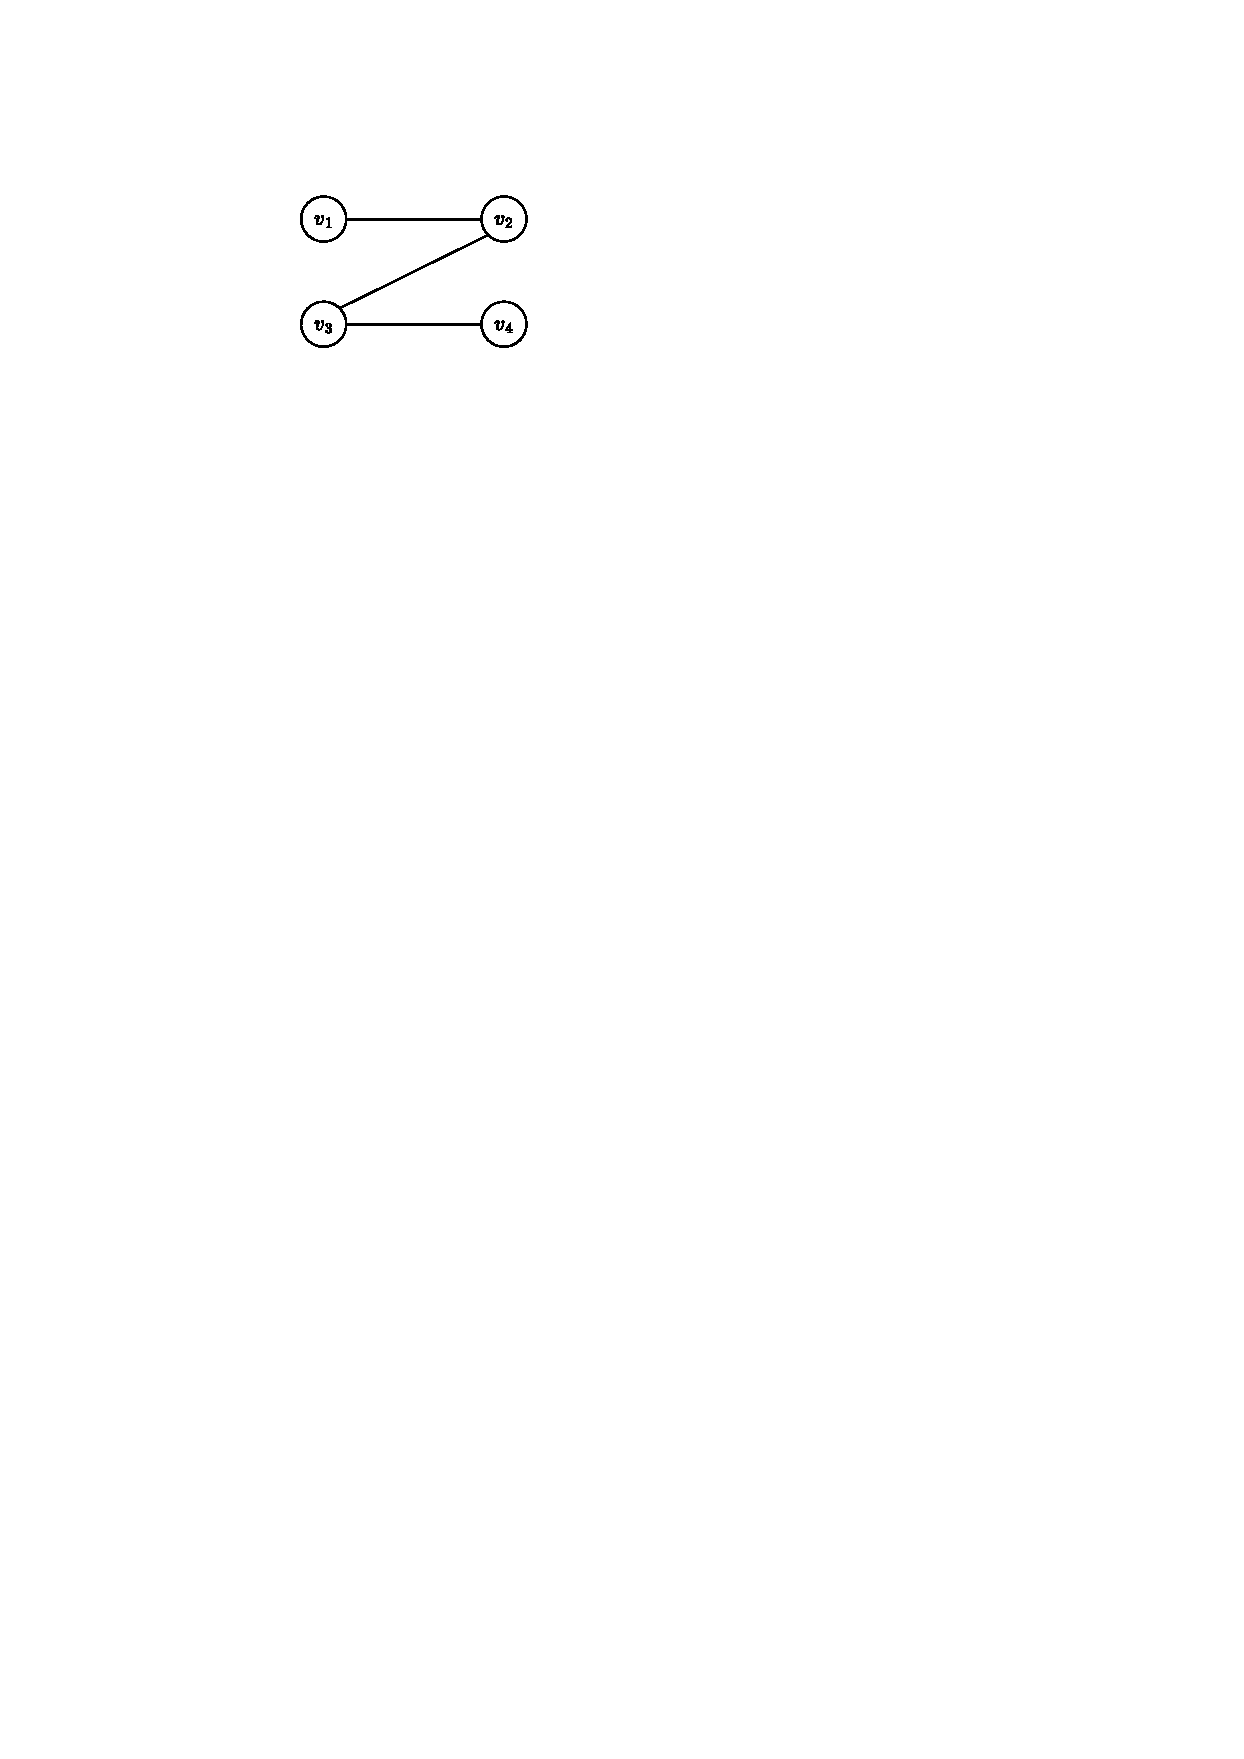
\includegraphics[width=5cm]{images/matching.pdf}
    \end{center}
    \caption{マッチング$M_1=\{v_1,v_2\},\{v_3,v_4\}\}$と$M_2=\{\{v_2,v_3\}\}$はどちらも極大である. \label{fig:matching}}
\end{figure}

\paragraph*{例6.}
グラフ$G=(V,E)$の頂点部分集合$U\subseteq V$は, $U$に属する任意の二頂点間に辺がある(すなわち$\binom{U}{2}\subseteq E$)とき, \emph{クリーク (clique)}\footnote{cliqueとは派閥を意味する英単語である.}という.
特に, 単一頂点からなる集合$\{u\}$や$\emptyset$もクリークである.
クリークの部分集合もまたクリークなので,
グラフ$G$の全てのクリークからなる頂点集合族を$\F$とすると, $(V,\F)$は単体複体である.
これをグラフの\emph{クリーク複体 (clique complex)}と呼ぶ.

\begin{definition}{リンクとスケルトン}{link and skelton}
    単体複体$X=(V,\F)$を考える.
    面$\sigma \in \F$の\emph{リンク (link)}とは単体複体$(V\setminus \sigma, \F_{\sigma})$であって集合族$\F_\sigma$が
    \[
        \F_\sigma = \cbra*{ \tau \setminus \sigma \colon \sigma \subseteq \tau \in \F }
    \]
    で与えられるものである.
    特に, 頂点$v\in X(0)$のリンクは$X_{\{v\}}$の代わりに$X_v$で表す.

    次元$k$以下の面の集合
    \[
        \F_k = \cbra*{ \sigma \in \F \colon \dim \sigma \le k}
    \]
    に対し$(V,\F_k)$を\emph{$k$-スケルトン ($k$-skelton)}という.
\end{definition}
\begin{figure}
    \begin{center}
    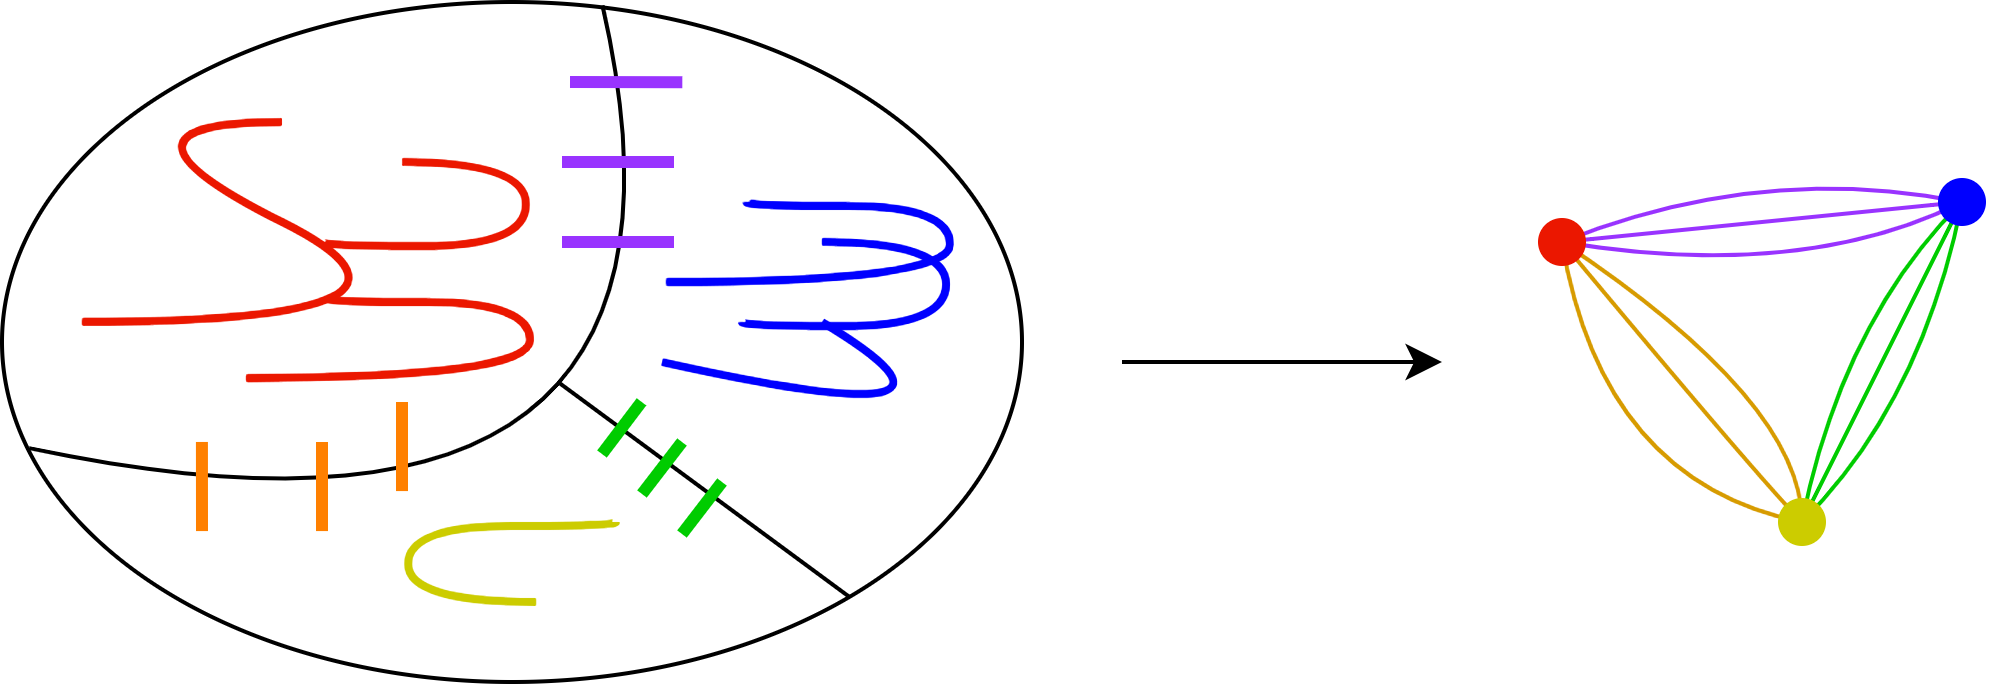
\includegraphics[width=12cm]{images/forest_link_shirnk.png}
    \caption{
        赤, 青, 黄の辺からなる森を$\sigma$としたとき, $\sigma$を縮約して得られるグラフ上の森がリンク$X_\sigma$の面に対応する.
        \label{fig:forest_link_shrink}.}
    \end{center}
\end{figure}
面$\sigma$のリンクとは, $\sigma$を「縮約」して得られる単体複体であり, 面$\sigma$の周りの局所的な構造を表している.
例えば連結グラフ$G=(V,E)$の森の全体からなる単体複体$X=(E,\F)$を考えよう.
$\sigma\in \F$を一つ固定したとき, リンク$X_\sigma$はどのような単体複体になっているだろうか?
$X_\sigma$の全ての面は辺集合$\sigma$を含むので, $\sigma$に含まれる全ての頂点を縮約して得られるより小さなグラフを考え, そこから$\sigma$の辺を除去して得られるグラフ$G'$の森全体からなる単体複体とみなせる (\cref{fig:forest_link_shrink}).
マトロイドの文脈では縮約と呼ばれる操作と同じである.

本講義では基本的に$1$-スケルトンのみ扱う.
単体複体の$1$-スケルトンは, $1$次元の面を辺とみなすことでグラフと同一視できる.
以後, $1$-スケルトンといった場合はこの同一視によってグラフとして扱う.

純粋な$d$次元単体複体$X$の面$\sigma\in X(i)$のリンク$X_\sigma$は純粋な$(d-i-1)$次元単体複体である.
特に$X_\emptyset = X$である.

%\end{definition}
\section{大域エクスパンダー性}
グラフ上のランダムウォークは頂点集合上で遷移するものを考えていたが,
単体複体上のランダムウォークは異なる次元の面の間で遷移するものを考える.
具体的には, \cref{sec:graph up and down walk}で考えたようにある次元$i$の面から次元$i+1$の面に遷移する上昇ウォークと逆に次元$i+1$の面から次元$i$の面に遷移する下降ウォークである.
上昇ウォークと下降ウォークが互いに随伴の関係になるようにするため, 各$X(i)$上での定常分布を定義し, $X(i)$と$X(i+1)$の間で詳細釣り合い条件が満たされるように定義される.

\subsection{下降ウォークと定常分布}
まず, \cref{sec:graph up and down walk}で考えた下降ウォークを単体複体に拡張し, $X(d)$上では一様分布を定常分布とすることによって帰納的に各$X(i)$上での定常分布を定める.
\begin{definition}{下降ウォークと面上の定常分布}{down walk and stationary distribution}
    $\pi$で重み付けられた純粋な$d$次単体複体$X=(V,\F)$を考える. 
    各$i=0,\dots,d$に対し
        確率行列$\Pdown_i \in [0,1]^{X(i) \times X(i-1)}$を
        \[
            \Pdown_i(\tau,\sigma) = \begin{cases}
                \frac{1}{i+1}	& \tif \sigma \subseteq \tau,\\
                0 & \totherwise
            \end{cases}
        \]
        とし, $X(i)$上の分布$\pi_i \in [0,1]^{X(i)}$を
        \begin{itemize}
        \item $i=d$のとき, $\pi_d = \pi$とする.
        \item $i<d$に対しては帰納的に$\pi_i = \pi_{i+1}\Pdown_{i+1}$とする.
        \end{itemize}
    各$i$に対し分布$\pi_i$を$X(i)$上の($i$次の)\emph{定常分布}と呼ぶ.

    以後, 面$X(i)$には暗に定常分布$\pi_i$が付随しているとする.
    すなわち, $u \sim X(i)$と書いた場合は$u\sim \pi_i$を意味する.
\end{definition}
面$\tau \in X(i+1)$に対して$\Pdown_{i+1}(\tau,\cdot)$で定まる$X(i)$上の分布は, 面$\tau$に含まれる頂点$u$を一様ランダムに選んだときの$\sigma = \tau \setminus\{u\}$の分布と等しい (\cref{fig:stationary_distribution}).
この分布は, まず定常分布に従って$X(d)$から面を選び, その中から一様ランダムに選ばれた$i+1$個の頂点からなる$X(i)$の面のなす分布でもある.
例えば$\pi$が一様分布のとき, $\pi_i(\sigma)$は$\sigma$を含む極大な面の個数に比例する.
これは遅延単純ランダムウォークの定常分布$\pi(u)$が次数$\deg(u)$に比例することの一般化である.

\begin{figure}[htbp]
    \begin{center}
    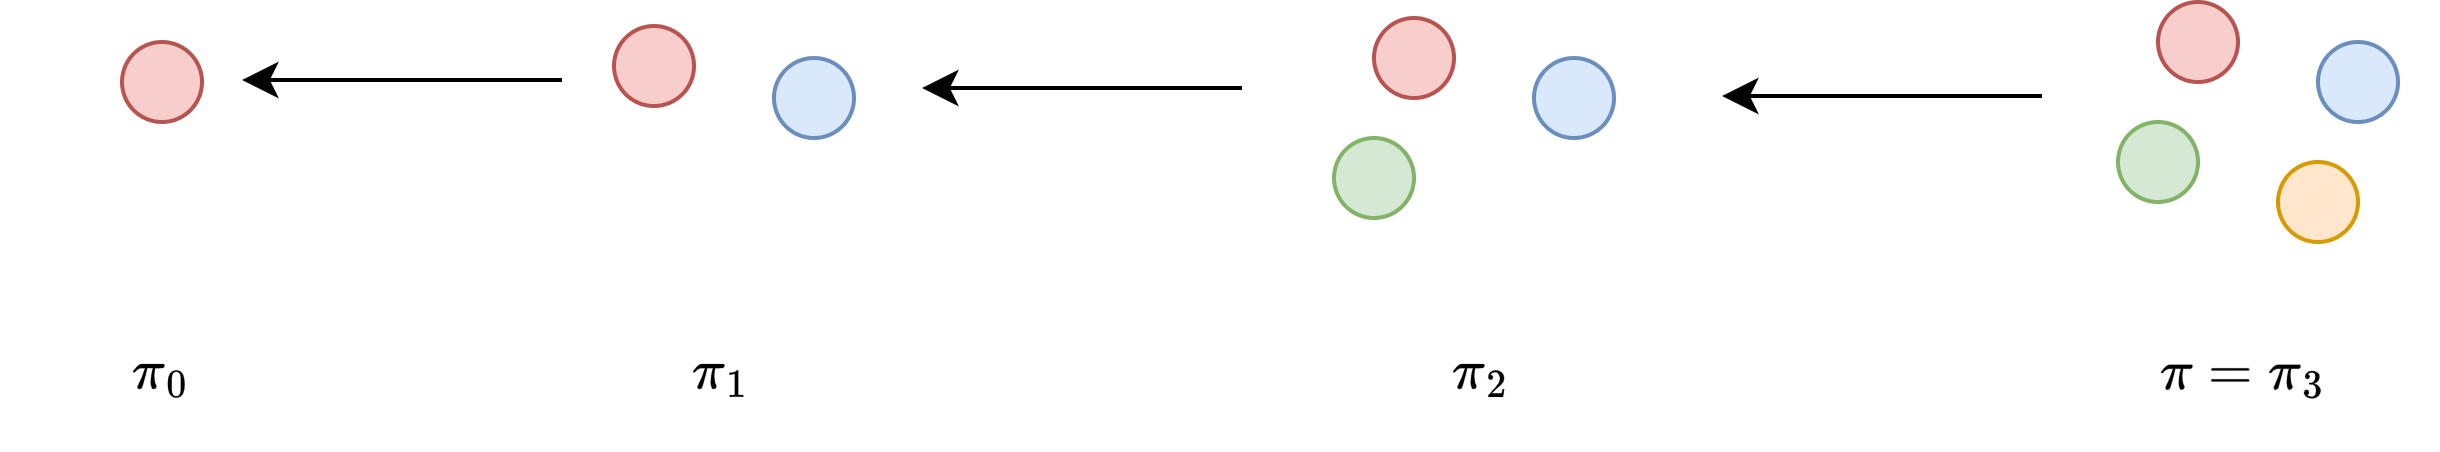
\includegraphics[width=\linewidth]{images/stationary_distribution.png}
    \caption{最大次の面を重み$\pi$に従ってランダムに選び, そこから一様ランダムな頂点を一つずつ消していくときの各次元での周辺分布が$\pi_i$となる. この仮定が下降ウォークである. \label{fig:stationary_distribution}}
    \end{center}
\end{figure}


ある面$\tau\in X(i+1)$から分布$\Pdown_{i+1}(\tau,\cdot)$に従ってランダムに選ばれた面$\sigma$に遷移する過程を\emph{下降ウォーク (down walk)}と呼ぶ.

各リンクに対しても同様に定常分布を定義する.
\begin{definition}{リンク上の定常分布}{link stationary distribution}
    純粋な$d$次元単体複体$X$のリンク$X_\sigma$ ($\sigma \in X(i)$)に対して最大次の定常分布$\pi^{\sigma}_{d-i-1}$を
    \begin{align*}
        \pi^\sigma_{d-i-1}(\alpha) &= \Pr_{\tau\sim\pi_{d}}\sbra*{\tau=\alpha\cup \sigma \condition \tau\supseteq \sigma}
    \end{align*}
    で定め, それ以下の次元の定常分布$\pi^\sigma_j$は\cref{def:down walk and stationary distribution}によって定める.

    以後, $u\sim X_\sigma(j)$と書いたとき, $u \sim \pi^\sigma_j$を意味する.
\end{definition}
リンク上の$j$次の定常分布$\pi^\sigma_j$は
\begin{align}
    \pi^\sigma_j(\alpha) = \Pr_{\tau \sim X(i+j+1)}\sbra*{\tau = \alpha \cup \sigma \condition \tau \supseteq \sigma} \propto \pi_{i+j+1}(\alpha\cup\sigma) \label{eq:pi alpha j}
\end{align}
を満たす.
特に$\sigma=\emptyset$とすれば, $i=\dim(\sigma)=-1$より$\pi^\emptyset_j = \pi_j$が成り立つ.

\begin{remark}{}{link of u}
    定義を咀嚼するために, ここでは頂点$u\in V$のリンク$X_u$に対して$0$次の定常分布を考えてみよう.
    $X_u(0)=\{v \in V \colon \{u,v\}\in X(1)\}$であり, これは$1$-スケルトンにおける$u$の隣接頂点の集合に等しい.
    ランダムな辺$e \sim X(1)$に対して端点のどちらか$v \sim e$を一様ランダムに選んだときの$v$の周辺分布が$\pi_0$となる.
    一方で, 固定した頂点$u$に対し, $u$を含むよう条件つけて$e \sim X(1)$をサンプリングしたとき, $u$でない方の端点$v$の分布が$\pi^u_0$となる.
    
    より高次元の面に対しても同様で, \cref{eq:pi alpha j}から分かるように, ある特定の面$\sigma$を含むよう条件つけられた状態で定常分布に従ってサンプリングしたときの$j$次の面の分布が$\pi^\sigma_j$である.
\end{remark}

\subsection{上昇ウォーク}
\cref{def:down walk and stationary distribution}では次元$i$の面から次元$i-1$に遷移する下降ウォークを与えた.
同様に, 次元$i$の面から次元$i+1$の面に遷移する上昇ウォークを, $X(i)$と$X(i+1)$の間の詳細釣り合い条件が成り立つように定義する.
%
\begin{definition}{上昇ウォーク}{up walk}
    純粋な$d$次単体複体$X=(V,\F)$を考える.
    各$i=-1,\dots,d-1$に対し
        確率行列$\Pup_i \in [0,1]^{X(i) \times X(i+1)}$を
    \begin{align*}
        \Pup_i(\sigma,\tau) &= \frac{\pi_{i+1}(\tau)}{\pi_i(\sigma)}\Pdown_{i+1}(\tau,\sigma) \\
        &= \begin{cases}
            \frac{\pi_{i+1}(\tau)}{(i+2)\pi_i(\sigma)}	& \tif \sigma\subseteq \tau,\\
            0 & \totherwise
        \end{cases}
    \end{align*}
    で定める\footnote{全ての$\sigma\in X(i)$に対し$\pi_i(\sigma)>0$である
    (そうでなければ, $\pi$の全成分が正であることに反する).
    }.
\end{definition}
%
簡単な計算により行列$\Pup_i$は確かに確率行列であることが確認できる.

二つの面集合$X(i)$と$X(i+1)$を部集合とする二部グラフを考えればわかりやすい.
それぞれの部集合には$\pi_i,\pi_{i+1}$が定常分布として付随しており,
上昇ウォーク$\Pup_i$と下降ウォーク$\Pdown_{i+1}$は詳細釣り合い条件
\[
    \forall \sigma\in X(i),\tau\in X(i+1),\,\pi_i(\sigma)\Pup_i(\sigma,\tau) = \pi_{i+1}(\tau)\Pdown_{i+1}(\tau,\sigma)
\]
を満たしている.

なお, 下降ウォーク$\Pdown_{i}$と上昇ウォーク$\Pup_i$の添字$i$は遷移の開始地点の面の次元としている.
%

\begin{figure}
    \begin{center}
    \includegraphics[width=10cm]{images/walks.png}
    \caption{上昇下降ウォーク$\PDU_i$と下降上昇ウォーク$\PUD_i$ \label{fig:walks}}
    \end{center}
\end{figure}
最後に, 上昇ウォークと下降ウォークを組み合わせることによって面$X(i)$上の二種類のランダムウォークを定義する (\cref{fig:walks}).
\begin{definition}{上昇下降と下降上昇ウォーク}{UD and DU walk}
    \cref{def:down walk and stationary distribution}, \ref{def:up walk}と同じ設定を考える.
    \begin{align*}
        &\PUD_i \defeq  \Pup_i \Pdown_{i+1},\\
        &\PDU_i \defeq \Pdown_{i}\Pup_{i-1}
    \end{align*}
    を遷移確率行列として持つ$X(i)$上のランダムウォークをそれぞれ\emph{上昇下降ウォーク (up-down walk), 下降上昇ウォーク (down-up walk)}と呼ぶ.
    ここで, $X(-1)$上での下降上昇ウォークと$X(d)$上での上昇下降ウォークは定義されない.
\end{definition}
上昇下降ウォークはグラフ上の遅延単純ランダムウォークの自然な一般化になっている (\cref{sec:graph up and down walk}).

\begin{remark}{「上昇」「下降」の名称}{up and down}
    非常にややこしいのだが,
    上昇ウォークと下降ウォークは遷移確率行列を左右どちらから作用させるかによって「上昇」「下降」の意味合いが反転してしまう.
    確率行列としての上昇ウォークは$\Pup_i \in [0,1]^{X(i)\times X(i+1)}$で表せる.
    左から作用させる作用素とみなすと
    $\Pup_i\colon \Real^{X(i+1)} \to \Real^{X(i)}$
    であるので, 上昇ウォークは次元を一つ落とす作用素に見えてしまうのである.
    下降ウォークについても同様である.
    特に上昇下降ウォーク$\PUD_i=\Pup_i\Pdown_{i+1}$を左から作用させると「次元を下げてから上げる」ものになるので, 下降上昇ウォークと混同しやすい.
    
    本講義はランダムウォークを主眼におき, 右から作用させるときの$\Pup_i,\Pdown_i$に興味があるので
    \cref{def:down walk and stationary distribution}, \ref{def:up walk}の呼称を採用している.
    ランダムウォークの遷移確率行列として扱う場合は右から作用させ, 
    内積空間を考え随伴性などを考える場合(\cref{sec:inaiseki})は左から作用させる (このときの行列$P$をマルコフ作用素と呼ぶことがある).

    なお, 可逆なランダムウォーク(\cref{def:reversible})は自己随伴性より, 内積$\piprod{\cdot,\cdot}$の意味では左右どちらから作用させても本質的に同じであるのでこのような煩雑な話は考えなくて良い.
\end{remark}

上昇下降ウォークの性質を述べていく.
\begin{lemma}{定常分布}{UD and DU stationary distribution}
    面$X(i)$上の上昇下降ウォークと下降上昇ウォークはどちらも$\pi_i$を定常分布としてもつ.
\end{lemma}
\begin{proof}
    計算によって簡単に確認できる.
    実際,
    \begin{align*}
        &\pi_i \PUD_i = \pi_i \Pup_i \Pdown_{i+1} = \pi_{i+1} \Pdown_{i+1} = \pi_i, \\
        &\pi_i \PDU_i = \pi_i \Pdown_i \Pup_{i-1} = \pi_{i-1}\Pup_{i-1} = \pi_i
    \end{align*}
    より主張を得る.
\end{proof}
\begin{lemma}{}{PUD seibun}
    上昇下降ウォーク$\PUD_i \in [0,1]^{X(i)\times X(i)}$の各成分は
        \[
            \PUD_i(\sigma,\sigma') = \begin{cases}
                \frac{\pi_{i+1}(\sigma\cup\sigma')}{(i+2)^2\pi_i(\sigma)}
                & \tif \sigma\cup\sigma'\in X(i+1),\\
                \frac{1}{i+2} & \tif \sigma=\sigma', \\
                0 & \totherwise.
            \end{cases}
        \]
\end{lemma}
\begin{exercise}{}{PUD calc}
    \cref{lem:PUD seibun}を示せ.
\end{exercise}


\subsection{各次元の内積空間} \label{sec:inaiseki}
各次元$i$に対して$X(i)$とそれに付随する定常分布を定義できたので, \cref{def:naiseki}の特殊ケースの内積空間を考えることができる.
\begin{definition}{}{naisexi simplicial complex}
    重み付き単体複体$X$の各次元の定常分布を$\pi_i \in [0,1]^{X(i)}$としたとき, $\pi_i$で重みつけられた内積を$\iprod{\cdot,\cdot}$で表す.
    すなわち, 
    \[
        \iprod{f,g} = \sum_{\sigma \in X(i)} \pi_i(\sigma) f(\sigma)g(\sigma)
    \]
    とする.
    また, $\Real^{X(i)}$に内積$\iprod{\cdot,\cdot}$を付随して定まる空間を$\ispace$とし,
    この内積が誘導するノルムを$\inorm{\cdot}$と表す.
\end{definition}
%
上昇ウォーク
$\Pup_i\colon \ispace[i+1] \to \ispace$
と下降ウォーク
$\Pdown_{i+1} \colon \ispace \to \ispace[i+1]$
は互いに随伴の関係にある.
すなわち, 任意の$f\in \ispace[i+1]$と$g\in \ispace$に対して
\begin{align}
    \iprod[X(i+1)]{\Pdown_{i+1} f,g} =
    \iprod{f,\Pup_{i}g}
    \label{eq:adjoint up and walk}
\end{align}
が成り立つ.
%
\begin{exercise}{}{adjoint check}
\cref{eq:adjoint up and walk}を確認せよ.
\end{exercise}

\begin{lemma}{半正定値性}{psd}
    各$i$に対して上昇下降ウォーク$\PDU_i$と下降上昇ウォーク$\PUD_i$は半正定値である.
\end{lemma}
\begin{proof}
    $\PDU_i$と$\PUD_{i-1}$は同じスペクトルを持つので$\PDU_i$についてのみ示せばよい.
    任意の$f\in\ispace$に対し,
    \begin{align*}
        \iprod{f,\PDU_i f} = \iprod{f,\Pdown_i \Pup_{i-1} f} = \iprod[X(i-1)]{\Pup_{i-1}f,\Pup_{i-1}f}\ge 0.
    \end{align*}
\end{proof};


また, リンク$X_\sigma$に対しても\cref{def:link stationary distribution}で定義した定常分布を用いて内積空間$\ispace[X_\sigma(i)]$を定義できる.

単体複体の大域的なエクスパンダー性を下降上昇ウォークのエクスパンダー性で定める.
\begin{definition}{大域エクスパンダー性}{global expander}
    純粋な$d$次元単体複体$X=(V,\F)$は,
    任意の$0\le i \le d$に対して$X(i)$上の下降上昇ウォーク$\PDU_i$が$\lambda_2(\PDU_i)\le \lambda_i$を満たすとき,
    \emph{大域$(\lambda_0,\dots,\lambda_{d})$-エクスパンダー (global $(\lambda_0,\dots,\lambda_{d})$-expander)}であるという.
%    特に, $\lambda_0=\dots=\lambda_{d-1}=\lambda$のとき, 大域$\lambda$-エクスパンダーという.
\end{definition}
エクスパンダーグラフ(\cref{def:expander})と比較すると, 片側(第二固有値)だけの上界だけでエクスパンダー性を定義しているが, \cref{lem:psd}より下からのバウンドがあるので上界だけの保証で十分だらかである.

本講義の目標は単体複体の大域エクスパンダー性を証明することである.
特にマトロイドと呼ばれる単体複体の大域エクスパンダー性はMihail--Vazirani予想\cite{balanced_matroids}と呼ばれる30年来の未解決問題であった\footnote{\cite{balanced_matroids}にはこの予想はMihailとVaziraniが立てたものらしいのだが, この予想を陽に述べた最初の文献は私が調べた限りでは\citet{balanced_matroids}であった.}
が, 2019年に\citet{ALOV24}に解決された.
詳細は\cref{chap:matroid}にて解説する.


\section{局所エクスパンダー性}
単体複体における局所的なランダムウォークを定義し, これに基づいて単体複体の局所エクスパンダー性を定義する.
また, 局所エクスパンダー性を確認するための非常に強力な定理としてOppenheimのトリクルダウン定理を証明する.

\subsection{局所的なランダムウォーク}
各リンク$X_\sigma$の$1$-スケルトン上での局所的な重み付きランダムウォークを考える.
重み付きランダムウォークについては\cref{def:weighted random walk}を参照されたい.
%
\begin{definition}{局所ランダムウォーク}{local random walk}
    純粋な$d$次元単体複体$X = (V,\F)$を考える.
    次元$i \le d-2$の面$\sigma \in \F$に対し,
        リンク$X_\sigma$の$1$-スケルトンを$G_\sigma = (V_\sigma,E_\sigma)$とする.
    このグラフの辺重み$w_\sigma\colon E_\sigma \to [0,1]$を
    \[ w_\sigma(e) = \pi_{i+2}(\sigma\cup e) \]
    で定め, これによって定まる$V_\sigma$上の重み付きランダムウォークを面$\sigma$に関する\emph{局所ランダムウォーク (local random walk)}と呼び%\footnote{このランダムウォークの概念は高次元エクスパンダーの文脈ではほぼ必ず登場するが, 特に標準的な用語が与えられてはいないので、「局所ランダムウォーク」という用語は本講義だけの局所的なものとする.}
    , 遷移確率行列を$P_\sigma\in [0,1]^{V_\sigma\times V_\sigma}$とする.
\end{definition}
%
必ずしも局所ランダムウォークが既約性や非周期性を持つとは限らない(すなわち, グラフ$G_\sigma$が非連結だったり二部グラフになりうる)が,
可逆性は必ず満たすことに注意せよ.

グラフ($1$次元単体複体)だと面$\emptyset$に対する局所ランダムウォークのみ定義できるが, これは上昇下降ウォーク(すなわち遅延単純ランダムウォーク)と同じである.
従って局所ランダムウォークの概念はより高次元の単体複体を考える際に意味を持つ.
簡単な計算から, 遷移確率行列$P_\sigma$の各成分は以下のように表せる.
\begin{lemma}{}{local RW seibun}
    面$\sigma \in X(i)$ (ただし$i\le d-2$) に関する局所ランダムウォークの遷移確率行列$P_\sigma$の各成分は
    \begin{align*}
        P_\sigma(u,v) &= \begin{cases}
            	\frac{\pi_{i+2}(\sigma\cup\{u,v\})}{(i+3)\pi_{i+1}(\sigma\cup\{u\})}& \tif \{u,v\}\in E_\sigma,\\
        0 & \totherwise.
        \end{cases}
    \end{align*}
\end{lemma}
%
\begin{exercise}{}{local RW seibun}
    \cref{lem:local RW seibun}を示せ.
\end{exercise}
%
%\begin{lemma}{}{local random walk stationary distribution}
%    遷移確率行列$P_\sigma$をもつ局所ランダムウォークの定常分布を$\pi_\sigma$とすると, 
%\end{lemma}
%
\subsection{局所エクスパンダー}
純粋な単体複体の局所的なエクスパンダー性を定義する.
任意の面$\sigma$に対し$G_\sigma$上での局所ランダムウォークの第二固有値が小さいとき, その単体複体は局所的エクスパンダー性をもつという.
\begin{definition}{局所エクスパンダー性}{local expander}
    純粋な$d$次元単体複体$X=(V,\F)$を考える.
    任意の$i=-1,0,\dots,d-2$と任意の面$\sigma\in X(i)$に対し
    $\lambda_2(P_\sigma)\le \gamma_i$を満たすとき,
    \emph{局所$(\gamma_{-1},\dots,\gamma_{d-2})$-エクスパンダー (local spectral $(\gamma_{-1},\dots,\gamma_{d-2})$-expander)}であるという.
    特に, $\gamma_{-1}=\dots=\gamma_{d-2} = \gamma$であるとき, 局所$\gamma$-エクスパンダーであるという.
\end{definition}
あくまでも$G_\sigma$の片側エクスパンダー性のみを議論していることに注意.
従って, 局所エクスパンダーだからといって$G_\sigma$上の局所ランダムウォークの混交時間が小さいとは限らない (そもそも二部グラフになりうるので, 一般に収束しない).


\paragraph*{例1. 三角形複体.}
グラフ$G=(V,E)$上の頂点数$3$以下のクリークからなる単体複体を$X$とする (\cref{sec:define simplicial complex}の例6参照).
頂点$u \in V$のリンク$X_u \defeq X_{\{u\}}$を考える.
$u$の隣接頂点の集合を$N(u)$とする.
$G$辺$\{u,v_1\},\{u,v_2\}\in E$に対し, $\{v_1,v_2\}\in E$のときに三角形$\{u,v_1,v_2\}$が単体複体$X$の面となる.
従って, リンク$X_u$は頂点$u$の誘導部分グラフ$G[N(u)\setminus\{u\}]$に等しい .
また, 全ての三角形に対し一様な重みを与えているため, $G_u$上のランダムウォークは単純ランダムウォークと同一である.
\begin{figure}
    \begin{center}
    \includegraphics[width=10cm]{images/localwalk1.png}
    \caption{頂点$u$のリンクの2-スケルトン$G_u$は頂点$u$の隣接頂点からなる誘導部分グラフである.}
    \end{center}
\end{figure}
\paragraph*{例2. 全域木複体.}
連結グラフ$G=(V,E)$上の森からなる辺集合$E$上の単体複体を$X$とする (\cref{sec:define simplicial complex}の例3参照).
極大でない森$\sigma\subseteq E$に対するリンクの$1$-スケルトン$G_F$を考える.
このグラフの頂点集合は$E\setminus \sigma$であり, $e_1,e_2 \in E \setminus \sigma$が$G_\sigma$上で辺をなすのは$\sigma \cup \{e_1,e_2\}$が森でありかつその時に限る.

さて, $G$の部分グラフ$(V,\sigma)$を考えよう ((\cref{fig:tree link}).).
森$\sigma$の非極大性からこの部分グラフは二つ以上の連結成分$C_1,\dots,C_\ell \subseteq V$からなる.
従って, $e_1,e_2\in E\setminus \sigma$が森であることの必要十分条件は$e_1,e_2$が同じ連結成分間を繋がないことである.
\begin{figure}
    \begin{center}
    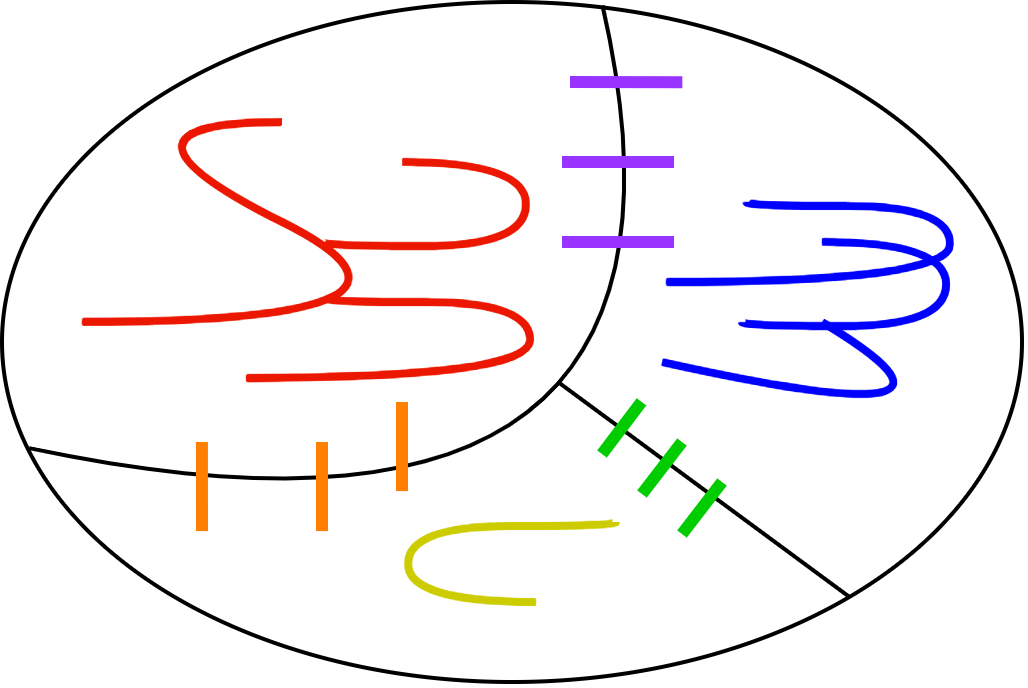
\includegraphics[width=8cm]{images/forest_link.png}
    \caption{赤, 青, 黄の辺からなる森を$\sigma$とする. 同じ連結成分の間を結ぶ二つの辺は$G_\sigma$上では隣接しない. \label{fig:tree link}}
    \end{center}
\end{figure}



\section{単体複体の局所大域原理}
単体複体における局所大域原理,
すなわち, 局所エクスパンダー性は大域エクスパンダー性を導くという結果は
比較的最近, \citet{KO20}によって証明された.
\begin{theorem}{Kaufman--Oppenheimの定理}{Kaufman-Oppenheim theorem}
    純粋な$d$-次元単体複体$X = (V,\F)$が局所$\gamma$-エクスパンダーならば,
    \[ \lambda_i = 1-\frac{1}{i+1} + \frac{\gamma i}{2}\]
    で定義された$\lambda_i$ ($i=0,\dots,d$) に対して$X$は大域$(\lambda_0,\dots,\lambda_{d})$-エクスパンダーである.
\end{theorem}
本節では\cref{thm:Kaufman-Oppenheim theorem}を証明する.

\subsection{非遅延上昇下降ウォーク}
\cref{thm:Kaufman-Oppenheim theorem}は, 各次元において$\PUD_i$と$\PDU_i$の固有値を比較することによって得られる.
$\PDU_i$と$\PUD_{i-1}$は随伴の関係にあるため非ゼロ固有値は一致する.
一方で, $\PUD_i$と$\PDU_i$は自己ループの影響もあり, その固有値を比較するのは難しい.
そこでまず, 上昇下降ウォーク$\PUD_i$から自己ループの遷移を除去したウォーク$\nonlazyPUD_i$を考え, $\nonlazyPUD_i$と$\PDU_i$の固有値を比較する.
\begin{definition}{非遅延上昇下降ウォーク}{nonlazy updown}
    \cref{def:down walk and stationary distribution}, \ref{def:up walk}と同じ設定において, 確率行列$\nonlazyPUD_i \in [0,1]^{X(i) \times X(i)}$を
    \[ \nonlazyPUD_i = \frac{i+2}{i+1}\rbra*{ \PUD_i - \frac{1}{i+2}I } \]
    とする. ここで$I$は$X(i)\times X(i)$の単位行列である.
\end{definition}
\cref{lem:PUD seibun}より$\PUD_i$に従うランダムウォークは確率$\frac{1}{i+2}$の自己ループを持つ.
従って$\PUD_i$から$\frac{1}{i+2}I$を引くと自己ループの確率は$0$になる.
しかしこうすると行和が$1-\frac{1}{i+2} = \frac{i+1}{i+2}$になるので, $\frac{i+2}{i+1}$倍して確率行列になるよう正規化したものが$\nonlazyPUD_i$である.
例えばグラフ上の単純遅延ランダムウォーク(\cref{def:lazy SRW})に対して同様の操作を行うと単純ランダムウォーク(\cref{def:SRW})を得る.
すなわち, グラフ$G$を$1$次元単体複体とみなしたときの$\nonlazyPUD_0$は$G$上の単純ランダムウォークと等しい.
\begin{remark}{\texorpdfstring{$\nonlazyPUD_i(\sigma,\cdot)$}{非遅延上昇下降ウォーク}のサンプリング}{nonlazyUPD sampling}
    \cref{lem:PUD seibun,lem:local RW seibun}より, 各成分は以下のように表せる:
    \begin{align*}
        \nonlazyPUD_i(\sigma,\sigma') = \begin{cases}
            \frac{1}{i+1}P_{\sigma\cap \sigma'}(\sigma\setminus\sigma',\sigma'\setminus\sigma)	& \tif \sigma\cup\sigma'\in X(i+1),\\
            0 & \totherwise.
        \end{cases}
    \end{align*}
    (ここでは$\sigma\setminus\sigma'$と$\sigma'\setminus\sigma$を頂点として扱っている).
    従って, 分布$\nonlazyPUD_i(\sigma,\cdot)$は以下のようにして生成できる:
    まず, 頂点$u \sim \sigma$を一様ランダムに選び, $\rho = \sigma\setminus\{u\}$とする.
    次に$v\sim P_\rho(u,\cdot)$に従って選び,
    $\rho\cup\{v\}$を出力する.
    実際, このようにして得られたランダムな面$\rho\cup\{v\}$は, $\sigma\cup\sigma'\in X(i+1)$なる$\sigma'$に対して以下が成り立つ:
    \begin{align*}
        \Pr\sbra*{\rho\cup\{v\} = \sigma'} &= \Pr\sbra*{ \rho = \sigma\cap \sigma' \tand v=\sigma'\setminus\sigma } \\
        &= \frac{1}{i+1}\cdot P_{\rho}(\sigma\setminus\sigma',\sigma'\setminus\sigma).
    \end{align*}
    
    また, 面$\emptyset$上の局所ランダムウォークの遷移確率行列$P_\emptyset$と$\nonlazyPUD_0$は一致する.
\end{remark}




\subsection{ランダムウォークの分解}
非遅延上昇下降ウォーク$\nonlazyPUD_i$と下降上昇ウォーク$\PDU_i$の固有値を比較するために,
これら二つのランダムウォークから得られる二次形式を局所ランダムウォークの二次形式に分解する.

%まず, 二次形式で考えるベクトル(関数)を各リンク上の制限に分解する.
\begin{definition}{}{restriction}
$f\in \ispace$と面$\sigma\in X(i-1)$に対し, $f_\sigma\colon X_\sigma(0) \to \Real$を以下で定める:
\[
    f_\sigma (u) = f(\sigma\cup\{u\}).
\]
\end{definition}
$\ispace$上の「大域的な」二次形式が各リンク$X_\sigma$上の「局所的な」二次形式の線形和で表せることを示す.
%
\begin{lemma}{}{nonlazyUP decomposition}
    純粋な$d$次元単体複体$X$と任意の$0 \le i\le d-1,f,g \in \ispace$に対し
    \[ \iprod{f, \nonlazyPUD_i g} = \E_{\rho\sim X(i-1)}\sbra*{ \iprod[X_\rho(0)]{f_\rho, P_\rho g_\rho} }. \]
%    ここで, $\pi^\rho_0 \in [0,1]^{X_\rho(0)}$はリンク$X_\rho$の頂点集合$X_\rho(0)$上の定常分布である.
\end{lemma}
\begin{proof}
\cref{rem:nonlazyUPD sampling}を用いて以下のように左辺を式変形していくと主張を得る:
\begin{align*}
    (\text{左辺}) &= \E_{\substack{\sigma\sim X(i) \\ \sigma'\sim \nonlazyPUD_i(\sigma,\cdot)}}\sbra*{ f(\sigma) g(\sigma')} \\
    &= \E_{\substack{\sigma\sim X(i)\\ u\sim \sigma,\\ \rho=\sigma\setminus\{u\} \\ v\sim P_\rho(u,\cdot)}}\sbra*{ f(\rho\cup\{u\}) g(\rho\cup\{v\}) } & & \text{$\because$\cref{rem:nonlazyUPD sampling} ($\sigma'=\rho\cup\{v\}$に対応)}\\
    &= \E_{\rho \sim X(i-1)}\sbra*{ \E_{\substack{ \sigma \sim X(i) \text{ conditioned on }\sigma\supseteq \rho \\ \{u\} = \sigma\setminus \rho \\ v \sim P_\rho(u,\cdot)}} \sbra*{ f_\rho(u) g_\rho(v) } } \\
    &=  \E_{\rho \sim X(i-1)}\sbra*{ \E_{\substack{u\sim X_\rho(0) \\ v \sim P_\rho(u,\cdot)}}\sbra*{f_\rho(u)g_\rho(v)}} & & \text{$\because$\cref{eq:pi alpha j}}\\
    &= (\text{右辺}).
\end{align*}
\end{proof}
下降上昇ウォークも同様に分解できる.
\begin{lemma}{}{DPwalk decomposition}
    純粋な$d$次元単体複体$X$と任意の$0\le i\le d,f,g\in \ispace$に対し,
    \begin{align*}
        \iprod{f,\PDU_i g}&= \E_{\rho\sim X(i-1)}\sbra*{ \E_{\pi^\rho_0}[f_\rho] \cdot \E_{\pi^\rho_0}[g_\rho] }.
%        &=  \E_{\rho\sim \pi_{i-1}}\sbra*{ \abra*{ f_\rho, J_\rho g }_{X_\rho(0)} }.
    \end{align*}
%    ここで, $J_\rho \in \Real^{X_\rho(0) \times X_\rho(0)}$は全ての行ベクトルが$\pi^\rho_0$に等しい, すなわち
%    $J_\rho(u,v) = \pi^\rho_0(v)$で定まる確率行列である.
\end{lemma}
\begin{proof}
上昇ウォークと下降ウォークの随伴性\cref{eq:adjoint up and walk}より以下のようにして得られる:
    \begin{align*}
        \iprod{f,\PDU_i g} &= \iprod{f,\Pdown_i \Pup_{i-1} g} \\
        &= \iprod[X(i-1)]{\Pup_{i-1}f, \Pup_{i-1}g } & & \text{$\because$\cref{eq:adjoint up and walk}} \\
        &= \E_{\rho \sim X(i-1)}\sbra*{ \E_{\substack{ \sigma,\sigma'\sim \pi_i\text{ conditioned on }\sigma,\sigma'\supseteq \rho }}\sbra*{f(\sigma)g(\sigma')} } \\
        &= \E_{\rho \sim X(i-1)}\sbra*{ \E_{u,v\sim X_\rho(0)}\sbra*{ f_\rho(u) g_\rho(v)} } \\
        &= \E_{\rho\sim X(i-1)}\sbra*{ \E_{\pi^\rho_0}[f]\cdot \E_{\pi^\rho_0}[g] }
    \end{align*}
\end{proof}

\subsection{第二固有値の比較}
\cref{thm:Kaufman-Oppenheim theorem}を証明するには$\lambda_2(\PDU_i)$を上から抑える必要がある.
そのためにまず$\lambda_2(\PDU_i)$と$\lambda_2(\nonlazyPUD_i)$を比較する.
\begin{lemma}{}{eigenvalue compare}
    純粋な$d$次元単体複体$X$が局所$\gamma$-エクスパンダーであるならば, 任意の$i=0,\dots,d$に対して
    \[ \lambda_2(\nonlazyPUD_i) \le \lambda_2(\PDU_i) + \gamma \]
    が成り立つ.
\end{lemma}
\begin{proof}
    $\PDU_i,\nonlazyPUD_i$はどちらも内積$\iprod{\cdot,\cdot}$に関して可逆なので,
    $\allone$に直交する任意の非ゼロの$f \in \ispace$に対し,
    \cref{lem:DPwalk decomposition,lem:nonlazyUP decomposition}より
    \begin{align*}
        \iprod{f,\nonlazyPUD_i f} - \iprod{f,\PDU_i f} &= \E_{\rho\sim X(i-1)}\sbra*{ \iprod[X_\rho(0)]{f_\rho, P_\rho f_\rho} - \E_{\pi^\rho_0}[f_\rho]^2}  \\
        & \le \E_{\rho \sim X(i-1)}\sbra*{\gamma \inorm[X_\rho(0)]{f_\rho - \E_{\pi^\rho_0}[f_\rho]}^2 } & & \text{$\because$\cref{lem:one side EML}} \\
        &\le \gamma \cdot \E_{\rho\sim X(i-1)}\sbra*{\inorm[X_\rho(0)]{f_\rho}^2} \\
        &= \gamma \inorm{f}^2.
    \end{align*}
    最後の等号は演習問題とする.
    移項して整理すると
    \begin{align*}
        \frac{\iprod{f,\nonlazyPUD_i f}}{\inorm{f}^2} &\le \frac{\iprod{f,\PDU_if}}{\inorm{f}^2} + \gamma \\
        & \le \lambda_2(\PDU_i) + \gamma & & \text{$\because$\cref{lem:Rayleigh quotient}}
    \end{align*}
    左辺は$f$に関して最大化すると$\lambda_2(\nonlazyPUD)$となるので主張を得る.
\end{proof}

\begin{exercise}{}{pinorm of f}
    上記の証明で用いた等式$\inorm{f}^2  = \E_{\rho \sim X(i-1)}\sbra*{\inorm[X_\rho(0)]{f_\rho}^2}$を示せ.
\end{exercise}

\begin{proof}[\textbf{\cref{thm:Kaufman-Oppenheim theorem}の証明.}]
    全ての$i=0,\dots,d$に対して$\lambda_2(\PDU_i) \le 1-\frac{1}{i+1} + \frac{\gamma i}{2}$を示せばよい.
    これを$i$に関する帰納法で示す.

    $i=0$のとき, $\PDU_0$を考える.
    $X(0)$上の任意の下降上昇ウォークは必ず面$\emptyset$に遷移し, その後に$X(0)$の頂点に遷移する.
    このときの遷移確率は$\pi_0$に従って選ばれる.
    従って$\PDU_0$は全ての行ベクトルが$\pi_0$であり, 特にランク$1$の行列なので, $\lambda_2(\PDU_0)=0$であり主張は正しい.

    一般の$i \ge 1$に対して
    \begin{align*}
        \lambda_2\rbra*{ \PDU_i } &= \lambda_2\rbra*{ \PUD_{i-1} } & & \text{$\because \lambda_2\rbra*{\Pdown_i\Pup_{i-1}}=\lambda_2\rbra*{\Pup_{i-1}\Pdown_i}$} \\
        &= \frac{i}{i+1}\lambda_2\rbra*{ \nonlazyPUD_{i-1} } + \frac{1}{i+1} & & \text{$\because$\cref{def:nonlazy updown}} \\
        &\le \frac{i}{i+1}\lambda_2\rbra*{ \PDU_{i-1}} + \frac{\gamma i + 1}{i+1} & & \text{$\because$\cref{lem:eigenvalue compare}}\\
        &\le \frac{i}{i+1} \rbra*{1 - \frac{1}{i} + \frac{(i-1)\gamma}{2}} + \frac{\gamma i + 1}{i+1} & & \text{帰納法の仮定} \\
        &= 1 - \frac{1}{i+1} + \frac{\gamma i}{2}.
    \end{align*}
    よって主張を得る.
\end{proof}

\subsection{Alev--Lauの定理}
\cref{thm:Kaufman-Oppenheim theorem}では, $\gamma < \frac{1}{d^2}$でなければ$\lambda_d$に対する非自明な上界が得られなかった.
この問題点は\citet{AL20}によって改善され以下の結果が示されている:
%
\begin{theorem}{Alev--Lauの定理}{ALev-Lau theorem}
    純粋な$d$-次元単体複体$X = (V,\F)$が局所$(\gamma_{-1},\dots,\gamma_{d-2})$-エクスパンダーならば,
    \[ \lambda_i = 1-\frac{1}{i+1}\prod_{j=-1}^{i-2}(1-\gamma_j)\]
    で定義された$\lambda_i$ ($i=0,\dots,d$) に対して$X$は大域$(\lambda_0,\dots,\lambda_{d-1})$-エクスパンダーである.
\end{theorem}

\chapter{マトロイド} \label{chap:matroid}
マトロイド(matroid)は「行列(matrix)のようなもの(-oid)」という名を冠するが,
ベクトルの線型独立性を拡張した独立性の概念として\citet{Whitney1935}によって定義された.

\section{定義}
\begin{definition}{マトロイド}{matroid}
    次の性質を持つ単体複体$(V,\F)$を\emph{マトロイド (matroid)}という:
    任意の$\sigma,\tau \in \F$に対し, $\abs{\sigma} < \abs{\tau}$ならば,
    ある$ u \in \tau \setminus \sigma$が存在して
    $\sigma \cup \cbra{u} \in \F$.

    マトロイド$(V,\F)$の面$\sigma\in \F$を特に\emph{独立集合 (independent set)}という.
\end{definition}

\begin{definition}{基}{basis}
    マトロイドの(包含関係に関して)極大な独立集合を\emph{基 (basis)}といい, 基全体の集合を$\B$で表す.
    特に断りのない限り, 基上の定常分布は一様分布とする.
\end{definition}
マトロイドは純粋な単体複体である.
実際, もし$\abs{B} < \abs{B'}$なる二つの基$B,B'\in\B$が存在するならば,
マトロイドの定義(\cref{def:matroid})より,
ある$u \in B'\setminus B$が存在して$B\cup \{u\} \in \F$とできるが,
これは$B$の極大性に矛盾する.

本講義ではマトロイドの基上の定常分布は常に一様分布とする.

\paragraph*{例1. 一様マトロイド}
\cref{eq:uniform matroid}で定まる単体複体$(V,\F)$は\emph{一様マトロイド (uniform matroid)}と呼ばれるマトロイドである.

\paragraph*{例2. グラフ的マトロイド}
\cref{eq:graphic matroid}で定まる単体複体$(V,\F)$はマトロイドである.
ここでは証明の概要を説明する.
マトロイドであることを示すには, 任意の二つの森$\sigma,\tau \in \F,\abs{\sigma} < \abs{\tau}$に対して, ある辺$e\in \tau\setminus \sigma$が存在して$\sigma\cup\{e\}$が閉路を含まないようにできることを言えばよい.
二つの森$\sigma,\tau \in \F,\abs{\sigma} < \abs{\tau}$を固定する.
森$\sigma\in \F$はグラフ上で複数の連結成分をなす.
これら連結成分の個数は$|V| - \abs{\sigma}$に等しい.
さて, 森$\tau$の中には, $\sigma$のなす連結成分のうち相異なる二つの間を横切る辺$e \in \tau \setminus \sigma$が存在する (\cref{fig:graphicmatroid}).
そうでなければ, $\tau$のなす連結成分の個数$|V|-\abs{\tau}$は$|V|-\abs{\sigma}$以下となってしまい, $\abs{\tau} > \abs{\sigma}$に矛盾.
この辺$e$を$\sigma$に追加しても閉路は発生しない.
(もし閉路$C$が生じるならば, $e$が$\sigma$のなす連結成分を横切ることに矛盾する).
すなわち, $\sigma\cup\{e\}\in\F$であり, 確かに$(V,\F)$はマトロイドである.
%
\begin{figure}
    \begin{center}
    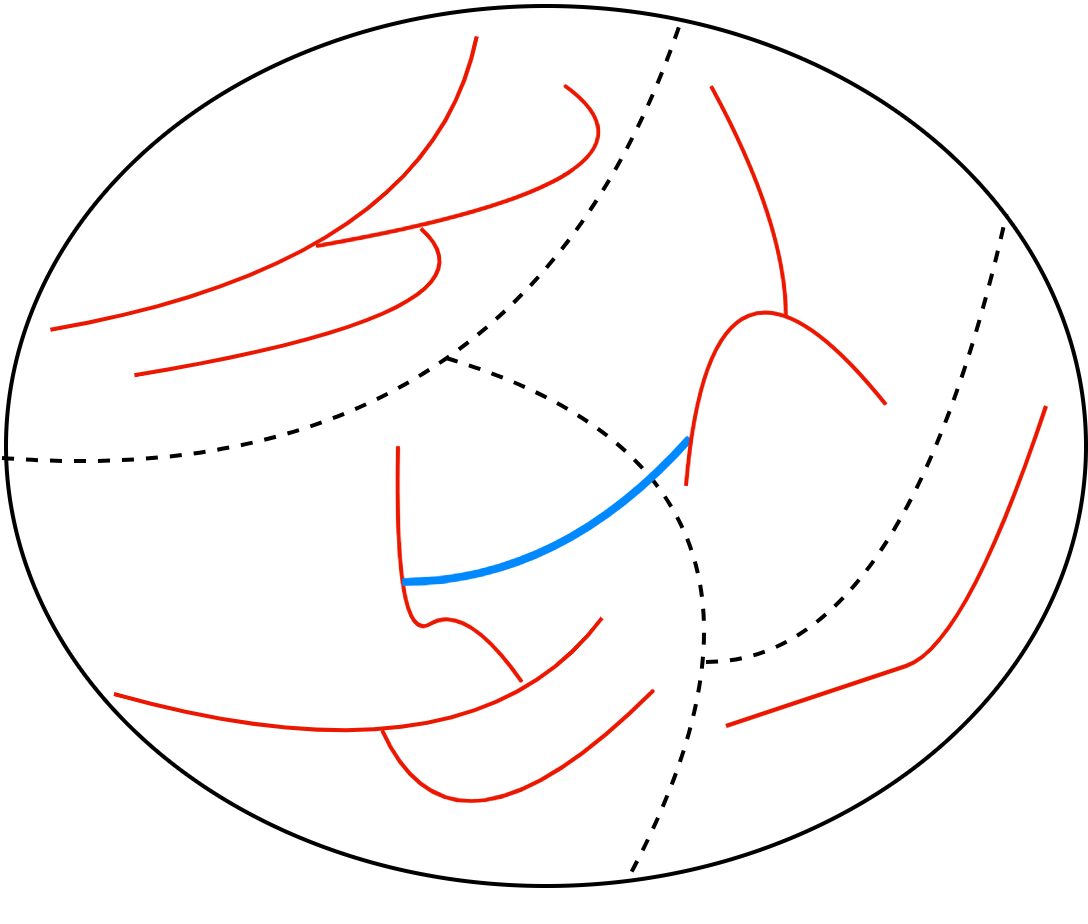
\includegraphics[width=7cm]{images/graphicmatroid.png}
    \caption{森$\sigma$のなす連結成分をまたがる辺$e \in \tau$が必ず存在する. \label{fig:graphicmatroid}}
    \end{center}
\end{figure}

グラフの森から定まる上記のマトロイドは\emph{グラフ的マトロイド (graphic matroid)}と呼ばれるマトロイドの重要なクラスをなす.

%
\paragraph*{例3. 線形マトロイド}
\cref{eq:linear matroid}で定まる単体複体$(V,\F)$は\emph{線形マトロイド (linear matroid)}と呼ばれるマトロイドである.
$\sigma,\tau\in \F$であって$\abs{\sigma} < \abs{\tau}$であるとする.
全てのベクトル$x\in \tau$が$x\in \mathrm{span}(\sigma)$に属するならば, $\tau$の線型独立性に矛盾するのであるベクトル$x\in \tau$が存在して$\{x\}\cup\sigma\in\F$となる.

\paragraph*{例4. 分割マトロイド}
有限集合$V$の分割$V=W_1\sqcup \dots \sqcup W_k$と非負整数$d_1,\dots,d_k\ge 0$を固定する.
部分集合族$\F$を
\begin{align}
    F \in \F \iff \forall i\in\{1,\dots,k\},\abs{W \cap W_i} \le d_i     \label{eq:partition matroid}
\end{align}
で定義したとき, $(V,\F)$は\emph{分割マトロイド (partition matroid)}と呼ばれるマトロイドである.
平たく言えば, 各$W_i$の元を高々$d_i$個ずつ含むものからなる部分集合族である.

\begin{exercise}{}{partition matroid}
    \cref{eq:partition matroid}で定まる単体複体$(V,\F)$がマトロイドであることを示せ.
\end{exercise}

\paragraph*{マトロイドでない例.}
クリーク複体やマッチング全体のなす単体複体はそもそも純粋とは限らないので必ずしもマトロイドになるとは限らない.

\section{基交換ウォーク}
\begin{definition}{基交換ウォーク}{basis-exchange walk}
    マトロイド$(V,\F)$の基上の下降上昇ウォークを\emph{基交換ウォーク (basis-exchange walk)}という.
\end{definition}
$X(d-1)$から$X(d)$への上昇ウォークを考えてみよう.
$\pi_{d-1}(\sigma)=\sum_{\tau\in\B} \pi_d(\tau) \cdot \Pdown_d(\tau,\sigma)$は, $\pi_d$が一様分布であり$\Pdown_d(\tau,\sigma)$は$\allone_{\tau\supset \sigma}$に比例するため, $\sigma$を含む基の個数に比例する.
従って
\begin{align*}
    \Pup_{d-1}(\sigma,\tau) = \frac{\pi_d(\tau)\Pdown_d(\tau,\sigma)}{\pi_{d-1}(\sigma)} \propto \allone_{\tau\supset \sigma}
\end{align*}
を得る.
すなわち, 基$B$から開始する基交換ウォークは,
一様ランダムに元$u\sim B$を選び,
$B\setminus u$を含む基の中から一様ランダムな基$B'\in B'$に遷移するランダムウォークであり, その定常分布は一様分布である.
基交換ウォークの混交時間のバウンドは長年の未解決問題であった.
\begin{conjecture}{Mihail--Vazirani予想}{Mihail-Vazirani}
    任意のマトロイド$M=(V,\F)$上の基交換ウォークの混交時間は$|V|$に関する多項式で上から抑えられる.
    すなわち, $M$に依存しないある定数$c>0$が存在して
    \[
        \tmix(1/2) \le |V|^c.
    \]
\end{conjecture}
基全体の個数は$\abs{V}$に関して指数関数的であるが,
ここでは
\emph{多項式ステップ}の基交換ウォークで混ざり合うかを問うている.
グラフ的マトロイドといった特殊ケースでは\cref{conj:Mihail-Vazirani}が正しいことが知られていた
\cite{balanced_matroids}が, 一般のマトロイドで正しいかどうかは未解決であった.

\section{マトロイドの局所エクスパンダー性}
本節では以下の定理を証明する.
\begin{lemma}{}{local expander matroid}
    任意のマトロイド$(V,\F)$は局所$0$-エクスパンダーである.
\end{lemma}


\subsection{Oppenheimのトリクルダウン定理}
ある単体複体$X$に対して局所エクスパンダー性(\cref{def:local expander})を示すには全ての面に対して$\lambda_2(P_\sigma)$を上から抑える必要がある.
一般にそもそも辺重み$w_\sigma$ (\cref{def:local random walk}) を求めることすら非自明であり, ましてや固有値を抑えるなど非常に大変な作業となる.
Oppenheimのトリクルダウン定理\cite{Oppenheim_tricling_down}は局所エクスパンダー性を確認するのに非常に有用な定理である.
\begin{theorem}{Oppenheimのトリクルダウン定理}{Oppenheim trickle-down theorem}
    純粋な重み付き$d$-次元単体複体$X = (V,\F)$が以下の二つを満たすとする:
    \begin{itemize}
    \item 全ての$i\le d-2$と全ての$\sigma\in X(i)$に対してグラフ$G_\sigma$は連結.
    \item 全ての$(d-2)$-次元の面$\tau \in X(d-2)$に対して$\lambda_2(P_\tau) \le \gamma$.
    \end{itemize}
    このとき, $\gamma_i \defeq \frac{\gamma}{1-(d-2-i)\gamma}$ ($i=-1,\dots,d-2$)に対して$X$は局所$(\gamma_{-1},\dots,\gamma_{d-2})$-エクスパンダーである.
\end{theorem}
端的に言えば, 次数$d-2$の面$\sigma \in X(d-2)$に対して$\lambda(P_\sigma)$を抑えれば全ての次元の面に対しても第二固有値が上から抑えられるという結果である.
最上次元の面のエクスパンダー性が下次元の面に波及していくという意味ではまさに「トリクルダウン(浸透)」といえよう.

一つ目のグラフ$G_\sigma$の連結性の条件は不可欠である.
例えば二つの完全グラフからなる非連結グラフ上の三角形複体を考えると,
空集合以外の全てのリンクは完全グラフ上のランダムウォークとなるため$\gamma=0$に対して二つ目の条件を満たすが, $\sigma=\emptyset$に対して$G_\sigma$は非連結であるため$\gamma_{-1}=0$にはならない.


\cref{thm:Oppenheim trickle-down theorem}は, まず$d=2$の特殊ケースで証明し, 一般の$d$についてはこの特殊ケースに帰着する.
%
\begin{lemma}{\texorpdfstring{$d=2$}{2次元}におけるトリクルダウン定理}{trickle-down for 2dim}
    純粋な重み付き$2$次元単体複体$X=(V,\F)$の各頂点$v\in X(0)$における局所ランダムウォーク$P_v$が$\lambda_2(P_v) \le \gamma$を満たし, かつその$1$-スケルトン$G_v$が連結ならば, 面$\emptyset$における局所ランダムウォーク$P_\emptyset$は
    \[
        \lambda_2(P_\emptyset) \le \frac{\gamma}{1-\gamma}
    \]
    を満たす.
\end{lemma}
この補題は本質的に$\gamma<1/2$のときに意味をなす.
\subsection{ランダムウォークの分解}
\cref{lem:trickle-down for 2dim}の証明は,
\cref{thm:Kaufman-Oppenheim theorem}と同様にランダムウォークを分解することから始まる.
記法の簡単のため, 頂点$u$のリンクを$X_{\{u\}}$の代わりに$X_u$, 遷移確率行列を$P_{\{u\}}$の代わりに$P_u$と表す.
\begin{definition}{}{localize}
    重み付き単体複体$(V,\F)$, 頂点$u\in V$, 関数$f \in \ispace[X(0)]$に対し,
    関数$f^u \in \ispace[X_u(0)]$を$f$の$X_u(0)$への制限, すなわち
    \[
        f^u (v) = f(v)
    \]
    とする.
\end{definition}
簡単な計算から以下の二次形式の分解補題が成り立つことがわかる.
\begin{lemma}{}{decomposition}
    任意の$f,g\in \ispace[X(0)]$に対して
    \[
        \iprod[X(0)]{f,g} = \E_{u\sim X(0)}\sbra*{ \iprod[X_u(0)]{f^u,g^u} }.
    \]
    また, 面$\emptyset$上の局所ランダムウォークの遷移確率行列を$P_\emptyset \in [0,1]^{X(0)\times X(0)}$とすると,
    \[
        \iprod[X(0)]{P_\emptyset f,g} = \E_{w\sim X(0)}\sbra*{ \iprod[X_u(0)]{P_uf^u,g^u} }.
    \]
\end{lemma}
\begin{proof}
    最初の等式を示す:
    \begin{align*}
        (\text{左辺}) &= \E_{u\sim X(0)} \sbra*{ f(u) g(u) } \\
        &= \E_{e \sim X(1)}\sbra*{ \E_{v \sim e} \sbra*{f(v)g(v)}} & & \text{$v\sim e$の周辺分布は$\pi_0$}\\
        &= \E_{u\sim X(0)} \sbra*{ \E_{\substack{e=\{u,v\} \sim X(1) \\ \text{conditioned on }e\ni u} }\sbra*{ f(v)g(v) }} & & \text{$e\sim X(1)$の$v$でない方の端点$u$を先に選ぶ}\\
        &= \E_{u\sim X(0)}\sbra*{ \E_{v \sim X_u(0)} \sbra*{f^u(v) g^u(v)} } & & \text{$\because$\cref{rem:link of u}}\\
        &= (\text{右辺}).
    \end{align*}
    二つ目の等式を示す.
    \begin{align*}
        (\text{左辺}) &= 
        \E_{\substack{u\sim X(0)\\ v\sim P_\emptyset(u,\cdot)}} \sbra*{ f(u)g(v)}\\
        &= \E_{t \sim X(2)}\sbra*{ \E_{\substack{w \sim t \\ u \sim t\setminus \{w\}, \\ \{v\}=t\setminus\{u,w\}}} \sbra*{f(u)g(v)} } \\
        &= \E_{w\sim X(0)}\sbra*{ \E_{\substack{t \sim X(2) \\ \text{conditioned on }t \ni w \\ u \sim t \setminus w \\ \{v\}=t\setminus\{u,w\}}} \sbra*{f(u)g(v)} } & & \text{前式の$w$の周辺分布は$X(0)$}\\
        &= \E_{w\sim X(0)}\sbra*{ \E_{\substack{u\sim X_w(0) \\ v\sim P_w(u,\cdot)}}\sbra*{f(u)g(v)} } \\
        &= (\text{右辺}).
    \end{align*}
\end{proof}
%
\begin{proof}[\textbf{\cref{lem:trickle-down for 2dim}の証明.}]
    記号の簡単のため$P=P_\emptyset$とする.
    局所ランダムウォーク$P$の第二固有値に対応する固有ベクトルを$f$とする.
    正規化して$\inorm[X(0)]{f}=1$とする.
    $P_\emptyset$の可逆性および\cref{lem:Rayleigh quotient}から,
    $\iprod[X(0)]{f,\allone}=0$である.
    補題を証明するには, $ \lambda_2(P)=\iprod[X(0)]{P f,f}$を上から抑えればよい.

    各頂点$u \in X(0)$に対し\cref{def:localize}で定義された$f^u \in \ispace[X_u(0)]$を考える.
    このベクトルを直交分解し,
    \begin{align}
        f^u = \alpha_u \allone^u + \overline{f^u} \label{eq:eigen decomposition fu}
    \end{align}
    と表す.
    ここで, $\allone^u \in \ispace[X_u(0)]$は全成分が$1$のベクトルで, $\alpha_u=\iprod[X_u(0)]{f,\allone^u}$であり, $\overline{f^u}$は$\allone^u$に直交するベクトルである.

    直交分解(\ref{eq:eigen decomposition fu})を用いると
    \begin{align*}
        \iprod[X_u(0)]{P_u f^u,f^u} &= \iprod[X_u(0)]{P_u\rbra*{\alpha_u\allone^u + \overline{f^u}}, \alpha_u\allone^u+\overline{f^u}} \\
        &= \iprod[X_u(0)]{\alpha_u \allone^u + P_u\overline{f^u}, \alpha_u\allone^u+\overline{f^u}} \\
        &= \alpha_u^2 + \iprod[X_u(0)]{P_u\overline{f^u},\overline{f^u}}  & & \text{直交性よりクロスタームは消える}\\
        &\le \alpha_u^2 + \gamma\inorm[X_u(0)]{\overline{f^u}}^2 & & \text{$\because$$\lambda_2(P_u)\le \gamma$および\cref{lem:Rayleigh quotient}}
    \end{align*}
    を得る.
    \cref{lem:decomposition}より,
    \begin{align*}
        \lambda_2(P) &= \iprod[X(0)]{Pf,f} \\
        &= \E_{u\sim X(0)}\sbra*{ \iprod[X_u(0)]{P_u f^u,f^u} } & & \text{$\because$\cref{lem:decomposition}の二つ目の等式} \\
        &\le \E_{u\sim X(0)}\sbra*{\alpha_u^2} + \gamma\cdot \E_{u\sim X(0)}\sbra*{\inorm[X_u(0)]{\overline{f^u}}^2} & & \text{直前の不等式を代入}\\
        &= \gamma\cdot \E_{u\sim X(0)}\sbra*{\alpha_u^2 + \inorm[X_u(0)]{\overline{f^u}}^2} + (1-\gamma)\cdot \E_{u\sim X(0)}\sbra*{\alpha_u^2} \\
        &= \gamma\cdot \E_{u\sim X(0)}\sbra*{\inorm[X_u(0)]{f^u}^2} + (1-\gamma)\cdot \E_{u\sim X(0)}\sbra*{\alpha_u^2} & & \text{$\because$$f^u$に対する三平方の定理}\\
        &= \gamma \cdot \inorm[X(0)]{f}^2 + (1-\gamma)\cdot \E_{u\sim X(0)}\sbra*{\alpha_u^2} & & \text{$\because$\cref{lem:decomposition}を$\iprod[X(0)]{f,f}$に適用} \\
        &= \gamma + (1-\gamma)\cdot \E_{u\sim X(0)}\sbra*{\alpha_u^2} & & \text{$f$のノルムは$1$}
    \end{align*}
    を得る.
    従って, $\E_{u\sim X(0)}\sbra*{\alpha_u^2}$を上から抑えたい.

    内積$\iprod[X_u(0)]{\cdot,\cdot}$の定義から
    \begin{align*}
        \alpha_u &= \iprod[X_u(0)]{f^u,\allone^u} \\
        &= \E_{v \sim X_u(0)}\sbra*{f^u(v)} \\
        &= \E_{v \sim X_u(0)}\sbra*{ f(v) } & & \text{\cref{def:localize}参照}\\
        &= (Pf)(u) & & \text{$P=P_\emptyset$は$1$-スケルトン上のランダムウォーク}
    \end{align*}
    であり, $f$は$P$の固有ベクトルなので
    \begin{align*}
        \E_{u\sim X(0)}\sbra*{\alpha_u^2} &= \inorm[X(0)]{Pf}^2 = \lambda_2(P)^2.
    \end{align*}
    これを代入すると二次不等式
    \begin{align*}
        \lambda_2(P) \le \gamma + (1-\gamma)\lambda_2(P)^2
    \end{align*}
    を得る. これを$\lambda_2(P)$について解くと
    \[
     \lambda_2(P)\ge 1 \text{ または }\lambda_2(P) \le \frac{\gamma}{1-\gamma}
    \]
    となるが, $1$-スケルトン$G_v$の連結性の仮定より$\lambda_2(P)<1$なので, $\lambda_2(P) \le \frac{\gamma}{1-\gamma}$を得る.    
\end{proof}
%
\subsection{トリクルダウン定理の証明}
\cref{lem:trickle-down for 2dim}を用いて一般の次元$d$に対する\cref{thm:Oppenheim trickle-down theorem}を証明する.
%
\begin{proof}[\textbf{\cref{thm:Oppenheim trickle-down theorem}の証明.}]
    $X=(V,\F)$を純粋な重み付き$d$次元単体複体とする ($d\ge 3$).
    面$\sigma \in X(d-3)$のリンク$X_\sigma$の次元は$2$であり,
    $X_\sigma$の頂点$v\in X_\sigma(0)$に対して
    $\sigma \cup \{v\} \in X(d-2)$より,
    $X_\sigma$上の$v$における局所ランダムウォークの遷移確率行列は$P_{\sigma\cup \{v\}}$に等しく, 仮定より$\lambda_2\rbra*{P_{\sigma\cup\{v\}}}\le \gamma$である.
    さらに, $X$の各リンクの$1$-スケルトンは連結なので, \cref{lem:trickle-down for 2dim}より
    \[
        \lambda_2(P_\sigma) \le \frac{\gamma}{1-\gamma}
    \]
    を得る.
    同じ議論を, $X$をその$(d-1)$-スケルトンに置き換えて適用すると,
    任意の$\sigma' \in X(d-4)$に対し
    \[
        \lambda_2(P_{\sigma'}) \le \frac{\frac{\gamma}{1-\gamma}}{1- \frac{\gamma}{1-\gamma}} = \frac{\gamma}{1-2\gamma}
    \]
    を得る.
    これを繰り返すと, ($j$に関する帰納法により)
    面$\rho \in X(d-2-j)$に対し
    \[
        \lambda_2(P_\rho) \le \frac{\gamma}{1-j\gamma}
    \]
    を得る.
\end{proof}
%


\section{Anari, Liu, Gharan, Vinzantの定理}
\begin{theorem}{Anari-Liu-Gharan-Vinzantの定理}{ALGV}
    任意のマトロイドは,
    \[ \lambda_i = 1-\frac{1}{i+1}\]
    に対して大域$(\lambda_0,\dots,\lambda_d)$-エクスパンダーである.
\end{theorem}
\begin{proof}
    次元$d$のマトロイド$X=(V,\F)$の独立集合$\sigma \in X(d-2)$を任意に固定し, リンク$X_\sigma$の$1$-スケルトン$G_\sigma$を考える.
    基$\B$上の定常分布は一様分布なので,
    $\sigma$に関する局所ランダムウォークは$G_\sigma$上の単純ランダムウォークとなる.
    さて, $G_\sigma$の頂点集合$V_\sigma$は
    \[V_\sigma = \{v\in V\setminus\sigma\colon \sigma\cup \{v\} \in \F\}\]
    であり,
    辺集合$E_\sigma \subseteq \binom{V_\sigma}{2}$は,
    \[
        E_\sigma = \cbra*{ \{u,v\}\colon \sigma\cup\{u,v\}\in \F }
    \]
    となる.

    ここで, 以下の命題を証明する:
    \begin{align}
        \{u,v\},\{v,w\}\not\in E_\sigma \Rightarrow \{u,w\} \not\in E_\sigma \label{eq:hogurahu clique}        
    \end{align}
    これは言い換えると$G_\sigma$の補グラフの全ての連結成分はクリークであることを意味する.
    命題(\ref{eq:hogurahu clique})を背理法で証明する.
    ある$\{u,v\},\{v,w\}\not\in E_\sigma$が存在して, さらに$\{u,w\}\in E$が成り立つと仮定する.
    このとき, $\tau\defeq \sigma\cup\{u,w\}\in \F$である.
    さらに, $v$は$G_\sigma$の頂点なので$\tau'\defeq \sigma\cup\{v\} \in \F$である.
    すなわち, $\tau,\tau'$は$\abs{\tau'} < \abs{\tau}$を満たす二つの独立集合なので, マトロイドの定義より
    ある$t \in \tau \setminus \tau' = \{u,w\}$に対して$\tau'\cup \{t\}=\sigma\cup\{u,t\} \in \F$, すなわち$\{u,t\}\in E_\sigma$となるが, これは$\{u,v\},\{v,w\}\not\in E$に矛盾する.

    主張(\ref{eq:hogurahu clique})より$G_\sigma$の補グラフの全ての連結成分はクリークである.
    これらを$C_1,\dots,C_\ell \subseteq V_\sigma$とし,
    $v_i\in \Real^{V_\sigma}$をクリーク$C_i$の指示ベクトルとする.
    $J\in\Real^{V_\sigma\times V_\sigma}$を全成分が$1$の行列とすると,
    $G_\sigma$の隣接行列$A\in\Real^{V_\sigma\times V_\sigma}$は
    \[
        A = J - \sum_{i=1}^\ell v_i v_i^\top
    \]
    となる.
    さらに, 局所ランダムウォークの定常分布$\pi^\sigma_0$を対角に並べた対角行列を$\Pi$とすると, 遷移確率行列は$P_\sigma = \Pi A = \Pi J - \sum_{i=1}^\ell \Pi v_iv_i^\top$となる.
    従って, 任意の$\iprod[V_\sigma]{f,\allone}=0$を満たす$f\in \ispace[V_\sigma]$に対して
    \begin{align*}
        \iprod[V_\sigma]{f,P_\sigma f} &= \iprod[V_\sigma]{f,\Pi J f} - \sum_{i=1}^\ell \iprod[V_\sigma]{f,\Pi v_iv_i^\top f} \\
        &= - \sum_{i=1}^\ell \iprod[V_\sigma]{f,\Pi v_iv_i^\top f} & & \text{$\because J f = 0$} \\
        &\le 0.
    \end{align*}
    最後の不等式では行列$\Pi v_iv_i^\top$が半正定値性を使った.
    これは,
    $\Pi v_i v_i^\top$がランク$1$行列であるため第二以降の固有値は全て$0$に等しく,
    さらに第一固有値はそのトレース$\mathrm{tr}(\Pi v_i v_i^\top) = \sum_{u\in V_\sigma} \pi^\sigma_0(u) v_i(u)^2\ge 0$に等しいことから従う.
    
    また, 全ての独立集合$\sigma\in \F$に対してリンク$X_\sigma$の$1$-スケルトン$G_\sigma$は連結である (演習問題).

    以上より, \cref{thm:Oppenheim trickle-down theorem}からマトロイド$X$は局所$0$-エクスパンダーであり, さらに$\gamma=0$として\cref{thm:Kaufman-Oppenheim theorem}を適用すると主張を得る.
\end{proof}

\begin{exercise}{}{matroid connectivity}
    任意のマトロイド$X = (V,\F)$の任意の独立集合$\sigma \in \F$に対し,
    リンク$X_\sigma$の$1$-スケルトン$G_\sigma$は連結であることを示せ.
\end{exercise}

\begin{corollary}{マトロイド上のランダムウォークの混交時間}{}
    次元$d$の任意のマトロイド$(V,\F)$上の基交換ウォークの混交時間は
    \[
        \tmix(\varepsilon) = (d+1)|V|\log\rbra*{\frac{1}{\varepsilon}}.
    \]
    特に, \cref{conj:Mihail-Vazirani}は真である.
\end{corollary}
\begin{proof}
    \cref{thm:ALGV}および$\PDU_d$の半正定値性より$\lambda(\PDU_d) \le 1-\frac{1}{d+1}$ であり, $\PDU_d$のスペクトルギャップ(\cref{def:second eigenvalue})は少なくとも$\frac{1}{d+1}$である.
    また, 基上の定常分布$\pi=\pi_d$は基上の一様分布であり, 特に$\pimin \ge 1/2^{|V|}$が成り立つので, \cref{lem:mixing time and spectral gap}より, 
    \[
        \tmix(\varepsilon) \le \frac{\log\rbra*{\frac{1}{2\pimin\varepsilon}}}{\log(1/\lambda(P))} \le (d+1)|V|\log\rbra*{\frac{1}{\varepsilon}}.
    \]
\end{proof}
\chapter{おわりに}
本講義ではまず, ランダムウォークの混交時間をスペクトルを用いて抑える方法を証明した.
次に, 単純ランダムウォークが高速に混交するグラフとしてエクスパンダーグラフを定義し,
エクスパンダー性の限界や理論計算機科学における応用を紹介した.
そして単体複体上のいくつかの種類のランダムウォークを定義し,
さらにこれに基づいてエクスパンダー性を定義した.
また, 単体複体のエクスパンダー性には局所的なものと大域的なものが定義でき,
局所的なエクスパンダー性から大域的なエクスパンダー性が導けることを示した (局所大域原理).
最後に応用としてトリクルダウン定理を用いてマトロイドのエクスパンダー性を議論し,
長年の未解決問題であったMihail--Vazirani予想の証明を与えた.

最後に, 高次元エクスパンダーの近年の進展について簡単に紹介する.
%
\section{左右ケイリー複体に基づく誤り訂正符号の構成}
$\Code\subseteq \mathbb{F}_2^n$を符号といい, 特に$\Code$が線形部分空間ならば線形符号という (定義については\cref{sec:error correcting code}参照).
線形符号$\Code$の次元を\emph{レート}と呼び,
相異なる二要素間の最小ハミング距離$\min_{x\neq y\in \Code}\dist(x,y)$を$\Code$の\emph{距離}という.
レートと距離がどちらも大きい符号が望ましいとされるが, これらのパラメータにはトレードオフがある.
理論計算機科学ではこれら二つの組合せ論的性質に加えて, 与えられた$w\in\mathbb{F}_2^n$が符号$\Code$に属するかどうかを効率的に判定できるという計算機科学的な性質(局所検査性; \citet{GS06})も重要である.
これら三つの性質を同時に
達成する符号の存在性はSpielmanの博士論文(1996)で
提起されて以来30年近く未解決であり, そのような符号は計算量理論において効率的な確率的検証可能証明(PCP)の構成などに応用される.
近年, \citet{DELLM22}はこの未解決問題を肯定的に解決した.
彼女らは, ケイリーグラフの概念を立方複体に自然に拡張した\emph{左右ケイリー立方複体 (left-right Cayley complex)}を導入し, それに基づく新たな符号を提案した.
この符号は\cite{SS96}によるエクスパンダーグラフに基づく符号(\cref{def:Cayley expander code})の自然な拡張である.

本講義で扱った高次元エクスパンダーはエクスパンダー性をもつ\emph{単体}複体であったが, \cite{DELLM22}で考えられている
左右ケイリー立方複体はある種のエクスパンダー性をもつ\emph{立方}複体である.
\citet{DELLM22}は, 立方複体の四角形が織り成す構造を\emph{テンソル符号}と呼ばれる二つの符号を合成する手法と巧妙に組み合わせることによって, 理論計算機科学の長年の未解決問題を解決することができたのである.
なお, 独立同時期に\citet{LH22,PK22}も同様の手法を用いてこの未解決問題を解決している.
\cite{LH22,PK22}に述べられているように, この手法は\emph{量子LDPC符号 (quantum LDPC code)}の構成にも応用されている \cite{LZ22}.
\renewcommand{\emph}[1]{\textit{#1}}
\printbibliography
%\appendix
%\input{appendix.tex}
\end{document}